\documentclass[web, english, gitmark, final]{thesissaclay}
%https://tex.stackexchange.com/questions/719543/how-do-i-add-icons-in-front-of-bibliography-entries
% https://tex.stackexchange.com/questions/563696/add-icons-to-bibliography-style-in-scrbook

\usepackage{subfiles}
\usepackage{nicefrac} 
%%%%%%%%%%%%%%%%%%%
%% CONFIGURATION %%
%%%%%%%%%%%%%%%%%%%
\title{Developping and exploring the interest of deep learning approaches in the field of multi-omics data}
\subtitle{Développer et explorer l'intérêt des approches de deep learning dans le domaine des données multi-omiques}
\author{Aurélien \textsc{Beaude}}

\date{XX month YYYY}
\location{Paris-Saclay}

\subject{Informatique}
\keywordsfr{apprentissage profond, multi-omiques, médecine personalisée}
\keywordsen{deep learning, multi-omics, personalized medicine}

\nnt{2024UPASA001}

\doctoralschool{STIC}
\graduateschool{Informatique et sciences du numérique}
\referee{Université d’Évry Val d’Essonne}
\unit{IBISC (Université Paris-Saclay, Univ Évry)}

%%%%%%%%%%%%%%%%%
%% SUPERVISORS %%
%%%%%%%%%%%%%%%%%
% order is important
\thesisdirector{\textbf{Blaise \textsc{Hanczar}}, Professeur}
%\thesiscodirector{}
\thesissupervisor{\textbf{Farida \textsc{Zehraoui}}, Maîtresse de conférence}
\thesisindustrysupervisor{\textbf{Franck \textsc{Augé}}, Docteur}

%%%%%%%%%%
%% JURY %%
%%%%%%%%%%
% Order is important, the jury table is filled according to the entry order
%\jurymember{firstname=Prénom, lastname=Nom, title=Titre, affiliation=Affiliation, role=Président}
\jurymember{firstname=Nistor, lastname=Grozavu, title=Professeur, affiliation={Université CY Cergy}, role=Rapporteur}
\jurymember{firstname=Laurent, lastname=Jacob, title=Directeur de recherche, affiliation={CNRS, Sorbonne Université}, role=Rapporteur}
\jurymember{firstname=Chloé-Agathe, lastname=Azencott, title=Professeure, affiliation={Mines Paris \textemdash PSL}, role=Éxaminatrice}
\jurymember{firstname=Laura, lastname=Cantini, title={Chargée de recherche}, affiliation={CNRS, Institut Pasteur}, role=Éxaminatrice}
\jurymember{firstname=Flora, lastname=Jay, title={Chargée de recherche}, affiliation={CNRS, Université Paris-Saclay}, role=Éxaminatrice}

%%%%%%%%%%%%%%%%%%%%%%%%%%
%% BIBLIOGRAPHY SOURCES %%
%%%%%%%%%%%%%%%%%%%%%%%%%%
\addbibresource{references.bib}
\addbibresource{my_publications.bib}
\addsectionbib[label=mypubli]{my_publications.bib}

%%%%%%%%%%%%%%%%%%
%% ABREVIATIONS %%
%%%%%%%%%%%%%%%%%%
\loadglsentries[type=\glsxtrabbrvtype]{preamble/abreviations}
%%%%%%%%%%%%%
%% SYMBOLS %%
%%%%%%%%%%%%%
\loadglsentries[type=symbols]{preamble/symbols}
%%%%%%%%%%%%%%
%% GLOSSARY %%
%%%%%%%%%%%%%%
\loadglsentries{preamble/glossary}
%%%%%%%%%%%
%% Maths %%
%%%%%%%%%%%
\setoperatorfont\mathrm%
\DeclareMathOperator{\softmax}{SoftMax}
\DeclareMathOperator{\enc}{Enc}
\DeclareMathOperator{\fcn}{FCN}
\DeclareMathOperator*{\argmax}{arg\,max}
\DeclareMathOperator*{\argmin}{arg\,min}
\DeclareMathOperator{\KL}{KL}
\DeclareMathOperator{\LN}{LN}
\DeclareMathOperator{\MHSA}{MHSA}
\DeclareMathOperator*{\E}{\symbb{E}}
\newcommand{\Tperm}{\ensuremath{\symcal{T}_{\pi}}}

%%%%%%%%%%%%%%%%%
%% Hyphenation %%
%%%%%%%%%%%%%%%%%
\hyphenation{%
    per-for-man-ces
    gen-ome
    com-ple-men-ta-ry
    con-tri-bu-tions
    re-pre-sen-ta-tion
    va-ria-tio-nal
    in-ter-pre-ta-bi-li-ty
    me-ta-bo-lo-mics
    train-ed
    me-di-ci-ne
    pre-dic-tion
    bio-mar-kers
    bio-mar-ker
    trans-for-ma-tion
    ar-chi-tec-tu-re
    through-put
    va-ria-tio-nal
    fra-me-work
    lear-n-ing
    mo-da-li-ty
    mo-da-li-ties
    di-men-sio-nal
    con-si-de-ring
    in-ter-ac-tions
    ex-pla-na-tions
    train-ed
    whe-re
    ar-chi-tec-tu-res
    Sub-ty-pe-For-mer
    pre-tr-ai-n-ed
}

\newcommand{\ie}{\textit{i}.\textit{e}.\ }%
\newcommand\mylabelformat[2][l]{\eqmakebox[listlabel@\EnumitemId][#1]{#2}}
\renewcommand*{\mkbibcompletename}[1]{%
	\ifitemannotation{highlight}
	{\textbf{#1}}
	{#1}%
}
\newcommand{\tableabbrev}[1]{\glsxtrshort{#1} = \glsxtrlong{#1}}

\usepgfplotslibrary{groupplots}
\usetikzlibrary{shadings, positioning, shapes.multipart, shapes.geometric, fit, shadows, backgrounds, shapes, shapes.misc, calc, intersections, arrows.meta, graphs, fadings, quotes, external}
\tikzset{
	square/.style={regular polygon,regular polygon sides=4}
}
\pgfplotsset{
	compat=1.18,
	every tick label/.append style={font=\footnotesize},
	every label/.append style={font=\small},
	every legend/.append style={font=\footnotesize, black},
	modelline/.style = {color = #1},
	% every axis/.append style={line width=1pt, tick style={line width=0.6pt}}
}
\pgfkeys{/pgf/number format/.cd,1000 sep={\,}}

\definecolor{attomicsclusteringColor}{HTML}{006e00}
\definecolor{attomicsgoColor}{HTML}{80BA5A}
\definecolor{attomicshallmarksColor}{HTML}{878500}
\definecolor{attomicsrandomColor}{HTML}{00bbad}
\definecolor{cnnColor}{HTML}{5954d6}
\definecolor{gcnCoExpColor}{HTML}{ff9287}
\definecolor{gcnPPIColor}{HTML}{d163e6}
\definecolor{mlpColor}{HTML}{000000}
\definecolor{RFColor}{HTML}{b80058}
\definecolor{SVMColor}{HTML}{ebac23}
\definecolor{xgboostColor}{HTML}{008cf9}

\pgfplotstableread[col sep=comma,]{data/attomics_perf.csv}\attomicsperf
\pgfplotstableread[col sep=comma,]{data/attomics_perf_zoom.csv}\attomicsperfzoom
\pgfplotstableread[col sep=comma]{data/CrossAttOmicsGateSelFreq.csv}\CrossAttOmicsGateSelFreq

\pgfplotstablegetrowsof{\attomicsperfzoom}
\pgfmathsetmacro{\Nattomicszoom}{\pgfplotsretval-1}

\newcommand{\attomicsline}[4]{
	\addplot [
		mark=*,
		color=#4,
		#3,
		mark options={solid},
		mark layer=like plot
	] plot [
			error bars/.cd,
			y dir=both,
			y explicit,
			error bar style={solid}
		] table [x={n_train_examples}, y={#1}, y error={#2}] {\attomicsperf};
}
\newcommand{\attomicslinecolor}[3]{%
	\IfSubStr{#1}{AttOmics}{
		\attomicsline{#1}{#2}{solid}{#3}
	}{
		\attomicsline{#1}{#2}{dashed}{#3}
	}
}
\newcommand{\attomicsplotomics}[1]{
	\pgfplotstableforeachcolumn\attomicsperf\as\col{%
		\IfBeginWith{\col}{#1}{%
			\StrSubstitute{\col}{y}{err}[\colerr]
			\StrBehind{\col}{#1}[\model]
			\IfStrEqCase{\model}{%
				{AttOmics - Clustering}{\attomicslinecolor{\col}{\colerr}{attomicsclusteringColor}}% chktex 8
					{AttOmics - GO}{\attomicslinecolor{\col}{\colerr}{attomicsgoColor}}% chktex 8
					{AttOmics - Hallmarks}{\attomicslinecolor{\col}{\colerr}{attomicshallmarksColor}}% chktex 8
					{AttOmics - Random}{\attomicslinecolor{\col}{\colerr}{attomicsrandomColor}}% chktex 8
					{CNN1d}{\attomicslinecolor{\col}{\colerr}{cnnColor}}% chktex 8
					{GCN - CoExp}{\attomicslinecolor{\col}{\colerr}{gcnCoExpColor}}% chktex 8
					{GCN - PPI}{\attomicslinecolor{\col}{\colerr}{gcnPPIColor}}% chktex 8
					{MLP}{\attomicslinecolor{\col}{\colerr}{mlpColor}}% chktex 8
					{RF}{\attomicslinecolor{\col}{\colerr}{RFColor}}% chktex 8
					{SVM}{\attomicslinecolor{\col}{\colerr}{SVMColor}}% chktex 8
					{XGBoost}{\attomicslinecolor{\col}{\colerr}{xgboostColor}}% chktex 8
			}
			\IfSubStr{#1}{mRNA}{\addlegendentryexpanded{\model}}{}
		}{}
	}
}

\newcommand{\plotattomicspoint}[4]{
	\addplot [
		mark=*,
		color=#4,
		only marks,
		mark options={solid},
		mark layer=like plot
	] plot [
			error bars/.cd,
			y dir=both,
			y explicit,
			error bar style={solid}
		] coordinates {(#1,#2) +- (0, #3)};
}
\newcommand{\plotattomicszoom}[1]{
	\pgfplotstableforeachcolumn\attomicsperfzoom\as\col{%
		\IfBeginWith{\col}{#1}{%
			\StrSubstitute{\col}{y}{err}[\colerr]
			\foreach \i in {0,...,\Nattomicszoom}{ % chktex 11
					\pgfplotstablegetelem{\i}{model}\of\attomicsperfzoom
					\edef\model{\pgfplotsretval}
					\pgfplotstablegetelem{\i}{\col}\of\attomicsperfzoom
					\pgfmathsetmacro{\y}{\pgfplotsretval}
					\pgfplotstablegetelem{\i}{\colerr}\of\attomicsperfzoom
					\pgfmathsetmacro{\yerr}{\pgfplotsretval}
					\ifdefempty{\y}{}{%
						\IfStrEqCase{\model}{%
							{AttOmics - Clustering}{\plotattomicspoint{\i}{\y}{\yerr}{attomicsclusteringColor}}% chktex 8
								{AttOmics - GO}{\plotattomicspoint{\i}{\y}{\yerr}{attomicsgoColor}}% chktex 8
								{AttOmics - Hallmarks}{\plotattomicspoint{\i}{\y}{\yerr}{attomicshallmarksColor}}% chktex 8
								{AttOmics - Random}{\plotattomicspoint{\i}{\y}{\yerr}{attomicsrandomColor}}% chktex 8
								{CNN1d}{\plotattomicspoint{\i}{\y}{\yerr}{cnnColor}}% chktex 8
								{GCN - CoExp}{\plotattomicspoint{\i}{\y}{\yerr}{gcnCoExpColor}}% chktex 8
								{GCN - PPI}{\plotattomicspoint{\i}{\y}{\yerr}{gcnPPIColor}}% chktex 8
								{MLP}{\plotattomicspoint{\i}{\y}{\yerr}{mlpColor}}% chktex 8
								{RF}{\plotattomicspoint{\i}{\y}{\yerr}{RFColor}}% chktex 8
								{SVM}{\plotattomicspoint{\i}{\y}{\yerr}{SVMColor}}% chktex 8
								{XGBoost}{\plotattomicspoint{\i}{\y}{\yerr}{xgboostColor}}% chktex 8
						}
					}

				}

		}{}
	}
}

%https://stackoverflow.com/questions/40768426/tikz-externalize-issue-when-using-pdflatex-with-output-directory
%\tikzexternalize[prefix=tikz/] 
% , system call/.append = {; pdfcrop --margins 1 "\image.pdf" "\image.pdf"}

\begin{document}
%%%%%%%%%%%%%%%%
%% TITLE PAGE %%
%%%%%%%%%%%%%%%%
\maketitle

\frontmatter

%%%%%%%%%%%%%%%%
%% ED SUMMARY %%
%%%%%%%%%%%%%%%%
\makesummary{./frontmatter/shortsummaryFR}{./frontmatter/shortsummaryEN}
%%%%%%%%%%%%%%%%
%% EXTRA INFO %%
%%%%%%%%%%%%%%%%
\thispagestyle{empty}
\vspace*{\fill}
\begin{center}
	
\includegraphics[scale=0.35]{logos/logo_sanofi_ibisc.pdf}
\end{center}
\vspace*{\fill}
\cleardoublepage{}

%%%%%%%%%%%%%%%%%%%%
%% FRENCH SUMMARY %%
%%%%%%%%%%%%%%%%%%%%
% Required by the university to write a summary of 4000 symbols when the main language is not the french.
\ifdefstring{\mainlanguagename}{french}{}{%
	\begin{french}
		\addchap{Résumé de la thèse --- French summary}
		La médecine de précision a transformé le domaine des soins, en adaptant les décisions à chaque patient.
L'essor de cette médecine a été rendu possible par le développement de méthodes de séquençage à haut débit, permettant la collecte de grandes quantités de données patients, et par le développement de méthodes d'apprentissage profond tirant parti de ces données.

La quantification des pools de molécules biologiques, comme l'acide désoxyribonucléique (ADN), les acides ribonucléiques (ARN), aussi connue sous le nom \textit{d'omiques}, permettent de mesurer systématiquement dans un échantillon biologique l’ensemble des molécules liées à une molécule biologique, par exemple l’expression de tous les gènes, ou transcriptomique.
La prédiction de phénotypes, comme un cancer, à partir de données omiques suscite de grands espoirs dans le développement de la médecine personnalisée.
Cependant, les données omiques sont des données de très grande dimension, avec plusieurs dizaines de milliers de variables, ce qui conduit à des modèles de grande taille, et bien que la disponibilité d'échantillons augmente, elle reste limitée pour des architectures de cette taille.
Les architectures actuelles, comme le perceptron multicouche, utilisent des poids fixes pendant l'inférence qui sont les mêmes pour tous les patients, limitant le potentiel d'une médecine véritablement personnalisée.
Les maladies comme le cancer résultent de perturbations de processus biologiques à de multiples niveaux.
Les méthodes d'acquisition actuelles permettent la collecte d'informations à tous les niveaux biologiques: génome, transcriptome, protéome, ouvrant la voie à des méthodes analytiques combinant ces informations pour améliorer les prédictions et la compréhension de ces maladies.
La compréhension des prédictions est essentielle dans les domaines à forts enjeux tels que la santé, cependant les modèles d'apprentissage profond sont considérés comme des \textit{boîtes noires}.
Pour remédier à ces limitations, nous avons proposé de nouvelles méthodes, qui sont énumérées ci-dessous.

Tout d'abord, nous avons développé AttOmics, un modèle pour les données omiques basé sur le mécanisme d'auto\-/attention.
Le mécanisme d'auto\-/attention permet la prise en compte d'interactions entre variables, l'expression de gènes par exemple, qui sont spécifiques à chaque patient.
De par la complexité en temps et en mémoire de l'attention et la grande dimension des données omiques, nous avons réduis la dimension des profils d'expressions en créant des groupes de variables.
Nous avons considéré plusieurs stratégies pour former les groupes: aléatoire, basé sur un clustering, ou la connaissance.
AttOmics fait au moins aussi bien que les autres méthodes d'apprentissage profond considérées: perceptron multicouche, réseaux de convolutions, réseaux de neurones pour les graphes.
En particulier, nous avons démontré l'avantage d'AttOmics pour des jeux d'entraînement avec peu d'exemples.
La visualisation des cartes d'attention permet l'identification des groupes importants pour un phénotype.

Dans un second travail, nous avons proposé CrossAttOmics, une architecture basée sur le mécanisme d'attention croisée pour combiner plusieurs omiques dans une unique représentation multimodale.
Chaque modalité est projetée dans un nouvel espace avec un encodeur spécifique basé sur le modèle AttOmics.
Le mécanisme d'attention croisée est utilisé pour calculer les interactions entre omiques.
Au lieu de considérer l'ensemble des interactions possibles, nous n'avons pris en compte que les interactions de régulation connues entre les modalités.
Cette approche peut être combinée avec des méthodes d'explicabilité comme \textit{layer-wise relevance (LRP)} pour identifier les interactions entre omiques les plus importantes.
Nous avons comparé notre approche avec de nombreuses méthodes d'apprentissage profond pour l'intégration de modalités: concaténation des omiques utilisé comme entrée d'un perceptron multicouche, de réseaux de neurones pour les graphes, d'Attomics ou bien la concaténation de représentations intermédiaires obtenues avec différentes architectures.

Dans un troisième travail, nous avons proposé CrossAttOmicsGate pour assigner un score à chaque interaction afin d'obtenir un modèle directement interprétable.
Le score d'interaction est obtenu avec un mécanisme de \textit{gating}, tout en forçant une majorité des scores à être nuls, favorisant l'interprétation.
De plus, les scores doivent être diversifiés entre patients pour refléter la diversité entre patients.
Ces deux propriétés, sparsité et diversité, sont assurées par l'ajout de quatre régularisations à la fonction de coût utilisée pour l'entraînement du modèle.

Enfin, nous avons développé un modèle génératif d'explications contrefactuelles, permettant d'identifier le changement requis dans le profil moléculaire pour qu'un patient soit en bonne santé.
L'explication contrefactuelle permet d'obtenir le changement minimal réaliste dans le profil d'expression changeant la prédiction faite par un modèle pré-entraîné.
Ce travail étant préliminaire, les résultats se concentrent sur la robustesse des modèles à des attaques adverses, la perturbation minimale d'une entrée trompant le réseau.

	\end{french}
}

%%%%%%%%%%%%%%%%%%%%%
%% ACKNOLEDGEMENTS %%
%%%%%%%%%%%%%%%%%%%%%
%\makeacknolegments{./frontmatter/acknolegments}

%%%%%%%%%%%%%%
%% LIST OFs %%
%%%%%%%%%%%%%%
\tableofcontents
\listoftables
\listoffigures
\printabbreviations
\printsymbols
\mainmatter
%%%%%%%%%%%%%%
%% CONTENTS %%
%%%%%%%%%%%%%%

%% Each chapter file must contain the following
%% \chapter{}
%% \graphicspath{{path/of/chapters_figures/}} % relative to main.tex
%% \dictum[author][citation] % to include a small quote at the begining of each chapter
%% \minitocpage % or \minitoc to display the content of the chapter
\subfileinclude{chapters/1-Introduction}
\subfileinclude{chapters/2-Background}
\subfileinclude{chapters/3-SOTA}
\subfileinclude{chapters/4-AttOmics}
\subfileinclude{chapters/5-CrossAttOmics}
\subfileinclude{chapters/6-CrossAttOmicsGate.tex}
\subfileinclude{chapters/7-Interpretability}
\subfileinclude{chapters/8-Conclusions}

\KOMAoption{parskip}{false}
\begin{singlespace}
	%%%%%%%%%%%%%%%%%%
	%% PUBLICATIONS %%
	%%%%%%%%%%%%%%%%%%
	\mypublications

	%%%%%%%%%%%%%%%%%
	%% BIBLIOGRAPY %%
	%%%%%%%%%%%%%%%%%
	\printbibheading
	\bibbysection[heading=subbibliography]
	\printglossary[title=Glossary]
\end{singlespace}
\KOMAoption{parskip}{half}
%%%%%%%%%%%%%%
%% APPENDIX %%
%%%%%%%%%%%%%%
\appendix
\pagestyle{appendix}
\addpart{Appendix}
\graphicspath{{figures/9-Appendix/}}
\chapter{Attention is equivariant to permutation}

\begin{definition}
	\(\pi \) is a permutation of \(n\)-elements.
	A transformation \(\symcal{T}_{\pi} : \symbb{R}^{n * d} \rightarrow \symbb{R}^{n \times d}\) is a spatial permutation if \(\Tperm\left(X\right) = P_{\pi}X\) where \(P_{\pi} \in \symbb{R}^{n\times n}\) is the permutation matrix associated with \(\pi \)
\end{definition}
rearrange rows of X
\( {\left[P_{\pi} \right]}_{ij} = e_{i, \pi(j)} = \begin{cases}
	1 & \text{if \(i = \pi(j)\)} \\
	0 & \text{else}
\end{cases}\)

\begin{property} %equivariance
	An operator \(A : \symbb{R}^{n * d} \rightarrow \symbb{R}^{n \times d}\) is equivariant to permutation if \(\forall X, \symcal{T}_{\pi}\)
	\[ \Tperm\left(A\left(X\right)\right) = A\left(\Tperm\left(X\right)\right) \]
\end{property}

\begin{property} %invariance
	An operator \(A : \symbb{R}^{n * d} \rightarrow \symbb{R}^{n \times d}\) is invariant to permutation if \(\forall X, \symcal{T}_{\pi}\)
	\[ \Tperm\left(A\left(X\right)\right) = \Tperm\left(X\right) \]
\end{property}

\begin{property}
	\[ \softmax\left(P_{\pi}XP_{\pi}^T\right) = P_{\pi}\softmax\left(X\right)P_{\pi}^T\]
\end{property}

% Permutation details
\begin{proof}
	\begin{align*}
		{\left[A\right]}_{ij} & = {\left[PA\right]}_{\pi(i)j}         \\
		                      & = {\left[AP^T\right]}_{i\pi(j)}       \\
		                      & = {\left[PAP^T\right]}_{\pi(i)\pi(j)}
	\end{align*}
\end{proof}

\begin{proof}
	\begin{align*}
		{\left[P_{\pi}\softmax\left(X\right)P_{\pi}^T\right]}_{\pi(i)\pi(j)} & = {\left[\softmax\left(X\right)\right]}_{ij}                                                                           \\
		                                                                     & = \frac{e^{{\left[X\right]}_{ij}}}{\sum e^{{\left[X\right]}_{ij}}}                                                     \\
		                                                                     & = \frac{e^{{\left[P_{\pi}XP_{\pi}^T\right]}_{\pi(i)\pi(j)}}}{\sum e^{{\left[P_{\pi}XP_{\pi}^T\right]}_{\pi(i)\pi(j)}}} \\
		                                                                     & = {\left[\softmax\left(P_{\pi}XP_{\pi}^T\right)\right]}_{\pi(i)\pi(j)}
	\end{align*}
\end{proof}

Let consider \(A_s\) the self attention operator defined as: \(\softmax\left[\left(XW^Q\right)\cdot{\left(XW^K\right)}^T \right]XW^V\)

\begin{theorem}
	Self-attention operator \(A_s\) is permutation equivariant
	\[\Tperm\left(A_s\left(X\right)\right) = A_s\left(\Tperm\left(X\right)\right)\]
\end{theorem}

\begin{proof}
	\begin{align*}
		A_s\left(\Tperm\left(X\right)\right) & = \softmax\left[ \left( \Tperm\left(X\right)W^Q\right) \cdot {\left(\Tperm\left(X\right)W^K\right)}^T \right] \Tperm\left(X\right)W^V \\
		                                     & = \softmax\left[ \left(P_{\pi}XW^Q\right)\cdot{\left(P_{\pi}XW^K\right)}^T  \right]P_{\pi}XW^V                                        \\
		                                     & = \softmax\left[ P_{\pi}\left(XW^Q\right)\cdot{\left(XW^K\right)}^T P_{\pi}^T  \right]P_{\pi}XW^V                                     \\
		                                     & = P_{\pi}\softmax\left[ \left(XW^Q\right)\cdot{\left(XW^K\right)}^T\right]P_{\pi}^{-1}P_{\pi}XW^V                                     \\
		                                     & = P_{\pi}A_S                                                                                                                          \\
		                                     & = \Tperm\left(A_s\left(X\right)\right)
	\end{align*}
\end{proof}

\chapter{Data used}
\section{TCGA}
\section{CCLE}

\chapter{AttOmics supplementary}\label{chap:attomics_appendix}
\begin{table}[htbp]
	\centering
	\caption{Distribution of the samples across cancer and splits}\label{tab:cancer_rep}
	\begin{tblr}{
		colspec={
				Q[l,m]
				Q[si={table-format=3,table-number-alignment=center},r]
				Q[si={table-format=3,table-number-alignment=center},r]
				Q[si={table-format=3,table-number-alignment=center},r]
				Q[si={table-format=3,table-number-alignment=center},r]
			},%
		row{1} = {guard, c, font=\bfseries},%
		row{2-Z} = {font=\small},%
		hline{1,Z} = {2pt},%
		hline{2,Y} = {1pt},%
				cell{Z}{1}={font=\bfseries},%
			}
		Cancer & Train & Validation & Test & Total \\
		BRCA   & 740   & 159        & 159  & 1058  \\
		UCEC   & 368   & 79         & 80   & 527   \\
		LGG    & 366   & 79         & 79   & 524   \\
		KIRC   & 355   & 76         & 77   & 508   \\
		THCA   & 354   & 76         & 76   & 506   \\
		LUAD   & 353   & 76         & 76   & 505   \\
		HNSC   & 344   & 74         & 74   & 492   \\
		PRAD   & 342   & 73         & 74   & 489   \\
		LUSC   & 331   & 71         & 71   & 473   \\
		SKCM   & 313   & 67         & 68   & 448   \\
		COAD   & 303   & 65         & 66   & 434   \\
		BLCA   & 282   & 60         & 61   & 403   \\
		OV     & 261   & 56         & 57   & 374   \\
		STAD   & 259   & 55         & 56   & 370   \\
		LIHC   & 257   & 55         & 56   & 368   \\
		Normal & 252   & 54         & 55   & 361   \\
		CESC   & 205   & 44         & 44   & 293   \\
		KIRP   & 200   & 43         & 44   & 287   \\
		SARC   & 182   & 39         & 39   & 260   \\
		LAML   & 67    & 15         & 15   & 97    \\
		Total  & 6134  & 1316       & 1327 & 8777
	\end{tblr}
\end{table}

\begin{table}[htbp]
	\centering
	\caption{Graph dimension for the GCN model}\label{tab:graph_dim}
	\begin{tblr}{
		colspec={
				Q[l,m]
				Q[l,m]
				Q[si={table-format=3,table-number-alignment=center},r]
				Q[si={table-format=3,table-number-alignment=center},r]
			},%
		row{1} = {guard, c, font=\bfseries},%
		row{2-Z} = {font=\small},%
		hline{1,Z} = {2pt},%
				hline{2} = {1pt},%
				hline{3} = {dashed, 1pt},
				cell{3}{1} = {r=3,c=1}{m},
			}
		Graph & Omics & Nodes & Edges  \\
		PPI   & mRNA  & 15985 & 234984 \\
		CoExp & mRNA  & 17951 & 400632 \\
		      & miRNA & 314   & 1051   \\
		      & DNAm  & 8360  & 390455
	\end{tblr}
\end{table}

\begin{table}[htbp]
	\centering
	\caption{Tested values of the hyper-parameters for the different architectures.}\label{tab:search_space}
	\begin{tblr}{
		colspec={
				Q[l,m]
				Q[l,m]
				Q[r,m]
			},%
		row{1} = {font=\bfseries},%
		row{2-Z} = {font=\small},%
		hline{1,Z} = {2pt},%
		hline{2} = {1pt},%
		hline{6,9,12,15,21} = {dashed, 1pt},%
				cell{2}{1} = {r=4,c=1}{l,m},%
				cell{6}{1} = {r=3,c=1}{l,m},%
				cell{9}{1} = {r=3,c=1}{l,m},%
				cell{12}{1} = {r=3,c=1}{l,m},%
				cell{15}{1} = {r=6,c=1}{l,m},%
				cell{21}{1} = {r=6,c=1}{l,m},%
			}
		Model         & Hyper-parameter     & Tested values                 \\
		MLP           & Nb layers           & \([ |1, 20 |]\)               \\
		              & Reduction ratio     & \([0.1, 0.9]\)                \\
		              & Dropout             & \([0,1]\)                     \\
		              & Batch norm.         & True/False                    \\
		CNN1d         & Kernel size         & 2,4,8                         \\
		              & Pooling size        & 2,4                           \\
		              & Num channels        & 32, 64, 128                   \\
		GNN           & Kernel size         & X, 2, 4, 8                    \\
		              & Num channels        & 1, 16, 32                     \\
		              & Readout             & concatenate, max, mean        \\
		SVM           & C                   & 0.1, 1, 10, 100, 1000         \\
		              & gamma               & 1, 0.1, 0.01, 0.001, 0.0001   \\
		              & Kernel              & rbf, linear, poly, sigmoid    \\
		Random Forest & n\_estimators       & \([1, 100]\)                  \\
		              & max\_features       & auto, sqrt                    \\
		              & max\_depth          & \([3, 20]\)                   \\
		              & min\_sample\_splits & 2, 5, 10, 15, 20, 25, 30, 50  \\
		              & min\_samples\_leaf  & 1, 2, 4, 6, 8, 10, 20, 30, 50 \\
		              & bootstrap           & True/False                    \\
		XGBoost       & n\_estimators       & \([1, 100]\)                  \\
		              & max\_depth          & 3, 4, 5, 6, 8, 10, 12, 15     \\
		              & gamma               & 0.0, 0.1, 0.2, 0.3, 0.4       \\
		              & min\_child\_weight  & 1, 3, 5, 7                    \\
		              & colsample\_bytree   & 0.3, 0.4, 0.5, 0.7            \\
		              & learning\_rate      & 0.05,0.10,0.15,0.20,0.25,0.30
	\end{tblr}
\end{table}

\begin{table}[htbp]
	\centering
	\caption{Selected hyper-parameters for the AttOmics architecture.}\label{tab:attomics_hparams}
	\begin{tblr}{
		colspec={
				Q[l,m]
				Q[l,m]
				Q[r,m]
				Q[r,m]
				Q[r,m]
			},%
		row{1} = {font=\bfseries},%
		row{2-Z} = {font=\small},%
		hline{1,Z} = {2pt},%
		hline{2} = {1pt},%
		hline{6,10} = {dashed, 1pt},%
				cell{2}{1} = {r=4,c=1}{l,m},%
				cell{6}{1} = {r=4,c=1}{l,m},%
				cell{10}{1} = {r=4,c=1}{l,m},%
			}
		Grouping   & Parameter  & mRNA                & DNAm           & miRNA   \\
		Random     & \# group   & 20                  & 10             & 5       \\
		           & \# blocks  & 4                   & 3              & 2       \\
		           & \# heads   & 1                   & 1              & 1       \\
		           & group size & 2164, 1459, 754, 50 & 1552, 826, 100 & 201, 80 \\
		Clustering & \# group   & 20                  & 20             & 10      \\
		           & \# blocks  & 4                   & 3              & 1       \\
		           & \# heads   & 1                   & 1              & 1       \\
		           & group size & 2164, 1459, 754, 50 & 776, 413, 50   & 50      \\
		GO         & \# group   & 46                  &                &         \\
		           & \# blocks  & 3                   &                &         \\
		           & \# heads   & 1                   &                &         \\
		           & group size & 200, 105, 10        &                &
	\end{tblr}
\end{table}

\begin{table}[htbp]
	\centering
	\caption{Architecture used for the models. X not applicable. For the GCN model a - kernel means convolution from spatial space, and \(>0\) means convolution in the spectral space}\label{tab:arch_other}
	\begin{tblr}{
		colspec={
				Q[l,m]
				Q[l,m]
				Q[r,m]
				Q[r,m]
				Q[r,m]
			},%
		row{1} = {font=\bfseries},%
		row{2-Z} = {font=\small},%
		hline{1,Z} = {2pt},%
		hline{2} = {1pt},%
		hline{5,9,12,15,18,24} = {dashed, 1pt},%
				cell{2}{1} = {r=3,c=1}{l,m},%
				cell{5}{1} = {r=4,c=1}{l,m},%
				cell{9}{1} = {r=3,c=1}{l,m},%
				cell{12}{1} = {r=3,c=1}{l,m},%
				cell{15}{1} = {r=3,c=1}{l,m},%
				cell{18}{1} = {r=6,c=1}{l,m},%
				cell{24}{1} = {r=6,c=1}{l,m},%
			}
		Model         & Parameter          & mRNA      & DNAm        & miRNA    \\
		MLP           & hidden dim         & 5739, 646 & 13675, 4103 & 807, 485 \\
		              & dropout            & 0         & 0           & 0        \\
		              & batch norm         & True      & True        & True     \\
		CNN --- 1D    & kernel             & 4         & 2           & 2        \\
		              & pooling            & 4         & 2           & 2        \\
		              & \# channels        & 64        & 64          & 64       \\
		              & stride             & 1         & 1           & 1        \\
		GNN --- PPI   & \# channels        & 1         & X           & X        \\
		              & kernel             & 2         & X           & X        \\
		              & readout            & concat    & X           & X        \\
		GNN --- CoExp & \# channels        & 1         & 1           & 1        \\
		              & kernel             & -         & -           & 2        \\
		              & readout            & concat    & concat      & concat   \\
		SVM           & kernel             & rbf       & rbf         & linear   \\
		              & gamma              & 0.0001    & 0.0001      & 1        \\
		              & C                  & 100       & 1000        & 0.1      \\
		RF            & n\_estimators      & 95        & 88          & 99       \\
		              & min\_samples       & 10        & 2           & 5        \\
		              & min\_samples\_leaf & 1         & 1           & 1        \\
		              & max\_features      & sqrt      & auto        & sqrt     \\
		              & max\_depth         & 18        & None        & 16       \\
		              & bootstrap          & False     & False       & False    \\
		XGBoost       & n\_estimators      & 88        & 18          & 66       \\
		              & min\_child\_weight & 7         & 7           & 7        \\
		              & max\_depth         & 15        & 4           & 15       \\
		              & learning\_rate     & 0.15      & 0.25        & 0.15     \\
		              & gamma              & 0         & 0.2         & 0.4      \\
		              & colsample\_bytree  & 0.5       & 0.5         & 0.5
	\end{tblr}
\end{table}

\begin{table}[htbp]
	\sisetup{separate-uncertainty-units=single, separate-uncertainty,detect-mode}
	\centering
	\caption{Models' sizes and their associated performances.}\label{tab:n_params_arch}
	\begin{tblr}{
		colspec={
				Q[l,m]
				Q[l,m]
				Q[r,m]
				Q[si={table-format=1.3(3),table-number-alignment=center, table-align-uncertainty = true}]
				Q[si={table-format=1.3(3),table-number-alignment=center, table-align-uncertainty = true}]
			},%
		row{1} = {guard, c},%
		row{2-Z} = {font=\small},%
		hline{1,Z} = {2pt},%
		hline{2} = {1pt},%
		hline{10,21} = {1pt, dashed},
				cell{2}{1} = {r=8,c=1}{l,m},
				cell{10}{1} = {r=11,c=1}{l,m},
				cell{21}{1} = {r=8,c=1}{l,m},
			}
		Omics & Model                   & \# of parameters & Error-Rate & C-Index   \\
		DNAm  & AttOmics --- Clustering & 28M              & 0.034(2)   & 0.722(10) \\
		      & AttOmics --- Random     & 62M              & 0.034(1)   & 0.721(5)  \\
		      & CNN1d                   & 93M              & 0.042(1)   & 0.720(8)  \\
		      & MLP                     & 367M             & 0.039(2)   & 0.718(2)  \\
		      & GNN --- CoExp           & 8.6M             & 0.037(3)   & 0.708(4)  \\
		      & SVM                     &                  & 0.034(0)   &           \\
		      & RF                      &                  & 0.050(3)   &           \\
		      & XGBoost                 &                  & 0.051(0)   &           \\
		mRNA  & AttOmics --- Clustering & 240M             & 0.043(2)   & 0.723(6)  \\
		      & AttOmics --- GO         & 28M              & 0.040(2)   & 0.721(5)  \\
		      & AttOmics --- Hallmarks  & 1.9M             & 0.046(3)   & 0.722(9)  \\
		      & AttOmics --- Random     & 240M             & 0.040(2)   & 0.726(6)  \\
		      & CNN1d                   & 470M             & 0.054(1)   & 0.714(6)  \\
		      & MLP                     & 333M             & 0.047(2)   & 0.717(6)  \\
		      & GNN --- CoExp           & 19M              & 0.047(2)   & 0.718(12) \\
		      & GNN --- PPI             & 16M              & 0.047(1)   & 0.722(3)  \\
		      & SVM                     &                  & 0.054(0)   &           \\
		      & RF                      &                  & 0.058(1)   &           \\
		      & XGBoost                 &                  & 0.035(0)   &           \\
		miRNA & AttOmics --- Clustering & 0.22M            & 0.071(4)   & 0.679(9)  \\
		      & AttOmics --- Random     & 0.68M            & 0.077(3)   & 0.668(2)  \\
		      & CNN1d                   & 6.6M             & 0.120(5)   & 0.677(4)  \\
		      & MLP                     & 1.7M             & 0.077(7)   & 0.669(11) \\
		      & GNN --- CoExp           & 0.37M            & 0.082(12)  & 0.697(13) \\
		      & SVM                     &                  & 0.034(0)   &           \\
		      & RF                      &                  & 0.050(3)   &           \\
		      & XGBoost                 &                  & 0.051(0)   &           \\
	\end{tblr}
\end{table}


\begin{table}[htbp]
	\sisetup{separate-uncertainty-units=single, separate-uncertainty,detect-mode}
	\centering
	\caption{Classification performances of the different models}\label{tab:perf_results}
	% TODO: longtblr
	\begin{tblr}{
		colspec={
				Q[l,m]
				Q[l,m]
				Q[si={table-format=1.3(3),table-number-alignment=center, table-align-uncertainty = true}]
				Q[si={table-format=1.3(3),table-number-alignment=center, table-align-uncertainty = true}]
				Q[si={table-format=1.3(3),table-number-alignment=center, table-align-uncertainty = true}]
				Q[si={table-format=1.3(3),table-number-alignment=center, table-align-uncertainty = true}]
				Q[si={table-format=1.3(3),table-number-alignment=center, table-align-uncertainty = true}]
				Q[si={table-format=1.3(3),table-number-alignment=center, table-align-uncertainty = true}]
			},%
		row{1} = {guard},%
		row{2-Z} = {font=\footnotesize},%
		hline{1,Z} = {2pt},%
		hline{2} = {1pt},%
		hline{10,21} = {1pt, dashed},
				cell{2}{1} = {r=8,c=1}{l,m},
				cell{10}{1} = {r=11,c=1}{l,m},
				cell{21}{1} = {r=8,c=1}{l,m},
			}
		Omics & Model                   & AUROC    & Accuracy  & F1-Score  & Precision & Recall    & Specificity \\
		DNAm  & AttOmics --- Clustering & 0.999(0) & 0.966(02) & 0.965(02) & 0.965(02) & 0.966(02) & 0.998(0)    \\
		      & AttOmics --- Random     & 0.999(0) & 0.966(01) & 0.964(02) & 0.963(02) & 0.966(01) & 0.998(0)    \\
		      & CNN1d                   & 0.998(0) & 0.958(01) & 0.956(01) & 0.955(01) & 0.958(01) & 0.998(0)    \\
		      & GCN --- CoExp           & 0.999(0) & 0.963(03) & 0.962(04) & 0.961(05) & 0.963(03) & 0.998(0)    \\
		      & MLP                     & 0.999(0) & 0.961(02) & 0.961(02) & 0.961(02) & 0.961(02) & 0.998(0)    \\
		      & RF                      & 0.998(0) & 0.950(03) & 0.950(03) & 0.950(03) & 0.950(03) & 0.997(0)    \\
		      & SVM                     & 0.998(0) & 0.966(00) & 0.966(00) & 0.966(00) & 0.966(00) & 0.998(0)    \\
		      & XGBoost                 & 0.997(0) & 0.949(00) & 0.949(00) & 0.949(00) & 0.949(00) & 0.997(0)    \\
		mRNA  & AttOmics --- Clustering & 0.999(0) & 0.957(02) & 0.956(02) & 0.956(02) & 0.957(02) & 0.998(0)    \\
		      & AttOmics --- GO         & 0.999(0) & 0.960(02) & 0.960(02) & 0.960(02) & 0.960(02) & 0.998(0)    \\
		      & AttOmics --- Hallmarks  & 0.999(0) & 0.954(03) & 0.954(04) & 0.953(04) & 0.954(03) & 0.998(0)    \\
		      & AttOmics --- Random     & 0.998(0) & 0.960(02) & 0.960(02) & 0.960(02) & 0.960(02) & 0.998(0)    \\
		      & CNN1d                   & 0.997(0) & 0.946(03) & 0.946(03) & 0.947(03) & 0.946(03) & 0.997(0)    \\
		      & GCN --- CoExp           & 0.999(0) & 0.953(02) & 0.953(02) & 0.954(02) & 0.953(02) & 0.998(0)    \\
		      & GCN --- PPI             & 0.999(0) & 0.953(01) & 0.953(01) & 0.954(02) & 0.953(01) & 0.998(0)    \\
		      & MLP                     & 0.997(0) & 0.953(02) & 0.954(02) & 0.955(02) & 0.953(02) & 0.998(0)    \\
		      & RF                      & 0.998(0) & 0.942(01) & 0.942(01) & 0.942(01) & 0.942(01) & 0.997(0)    \\
		      & SVM                     & 0.997(0) & 0.946(00) & 0.946(00) & 0.946(00) & 0.946(00) & 0.997(0)    \\
		      & XGBoost                 & 0.999(0) & 0.965(00) & 0.965(00) & 0.965(00) & 0.965(00) & 0.998(0)    \\
		miRNA & AttOmics --- Clustering & 0.997(0) & 0.929(04) & 0.927(04) & 0.927(05) & 0.929(04) & 0.996(0)    \\
		      & AttOmics --- Random     & 0.996(0) & 0.923(03) & 0.922(03) & 0.923(03) & 0.923(03) & 0.996(0)    \\
		      & CNN1d                   & 0.990(0) & 0.880(05) & 0.875(05) & 0.875(06) & 0.880(05) & 0.994(0)    \\
		      & GCN --- CoExp           & 0.995(1) & 0.918(12) & 0.915(13) & 0.914(13) & 0.918(12) & 0.996(1)    \\
		      & MLP                     & 0.995(0) & 0.923(07) & 0.923(07) & 0.924(08) & 0.923(07) & 0.996(0)    \\
		      & RF                      & 0.997(0) & 0.941(02) & 0.941(02) & 0.941(02) & 0.941(02) & 0.997(0)    \\
		      & SVM                     & 0.994(0) & 0.924(00) & 0.924(00) & 0.924(00) & 0.924(00) & 0.996(0)    \\
		      & XGBoost                 & 0.998(0) & 0.956(00) & 0.956(00) & 0.956(00) & 0.956(00) & 0.998(0)
	\end{tblr}
\end{table}

\begin{sidewaystable}
	\centering
	\caption{P-value from the t-test on the error rate of the different models}\label{tab:pval_error_rate}
	\begin{tabular}{llrrrrrrrrrr}
		\toprule
		omics                  & Model                   & AttOmics --- GO & AttOmics --- Hallmarks & AttOmics --- Random & CNN1d & GCN --- CoExp & MLP      & RF    & SVM      & XGBoost  & GCN --- PPI \\
		\midrule
		\multirow{7}{*}{DNAm}  & AttOmics --- Clustering & -               & -                      & 1.00                & 0.083 & 0.083         & 0.083    & 0.083 & 0.648    & 0.083    & -           \\
		                       & AttOmics --- Random     & -               & -                      & -                   & 0.083 & 0.381         & 0.083    & 0.083 & 0.648    & 0.083    & -           \\
		                       & CNN1d                   & -               & -                      & -                   & -     & 0.083         & 0.083    & 0.083 & 0.083    & 0.083    & -           \\
		                       & GCN --- CoExp           & -               & -                      & -                   & -     & -             & 0.510417 & 0.083 & 0.159091 & 0.083    & -           \\
		                       & MLP                     & -               & -                      & -                   & -     & -             & -        & 0.083 & 0.083    & 0.083    & -           \\
		                       & RF                      & -               & -                      & -                   & -     & -             & -        & -     & 0.083    & 0.648148 & -           \\
		                       & SVM                     & -               & -                      & -                   & -     & -             & -        & -     & -        & 0.083    & -           \\
		\midrule
		\multirow{10}{*}{mRNA} & AttOmics --- Clustering & 0.219           & 0.149                  & 0.078               & 0.078 & 0.078         & 0.078    & 0.078 & 0.078    & 0.078    & 0.078       \\
		                       & AttOmics --- GO         & -               & 0.149                  & 0.828               & 0.078 & 0.078         & 0.078    & 0.078 & 0.078    & 0.078    & 0.078       \\
		                       & AttOmics --- Hallmarks  & -               & -                      & 0.078               & 0.078 & 0.661         & 0.661    & 0.078 & 0.078    & 0.078    & 0.661       \\
		                       & AttOmics --- Random     & -               & -                      & -                   & 0.078 & 0.078         & 0.078    & 0.078 & 0.078    & 0.078    & 0.078       \\
		                       & CNN1d                   & -               & -                      & -                   & -     & 0.078         & 0.078    & 0.078 & 0.828    & 0.078    & 0.078       \\
		                       & GCN --- CoExp           & -               & -                      & -                   & -     & -             & 0.501    & 0.078 & 0.078    & 0.078    & 0.661       \\
		                       & GCN --- PPI             & -               & -                      & -                   & -     & -             & 1.00     & 0.078 & 0.078    & 0.078    & -           \\
		                       & MLP                     & -               & -                      & -                   & -     & -             & -        & 0.078 & 0.078    & 0.078    & -           \\
		                       & RF                      & -               & -                      & -                   & -     & -             & -        & -     & 0.078    & 0.078    & -           \\
		                       & SVM                     & -               & -                      & -                   & -     & -             & -        & -     & -        & 0.078    & -           \\
		\midrule
		\multirow{7}{*}{miRNA} & AttOmics --- Clustering & -               & -                      & 0.159               & 0.092 & 0.159         & 0.159    & 0.092 & 0.092    & 0.092    & -           \\
		                       & AttOmics --- Random     & -               & -                      & -                   & 0.092 & 0.510         & 1.00     & 0.092 & 0.673    & 0.092    & -           \\
		                       & CNN1d                   & -               & -                      & -                   & -     & 0.092         & 0.092    & 0.092 & 0.092    & 0.092    & -           \\
		                       & GCN --- CoExp           & -               & -                      & -                   & -     & -             & 0.673    & 0.092 & 0.510    & 0.092    & -           \\
		                       & MLP                     & -               & -                      & -                   & -     & -             & -        & 0.092 & 1.00     & 0.092    & -           \\
		                       & RF                      & -               & -                      & -                   & -     & -             & -        & -     & 0.092    & 0.092    & -           \\
		                       & SVM                     & -               & -                      & -                   & -     & -             & -        & -     & -        & 0.092    & -           \\
		\bottomrule
	\end{tabular}
\end{sidewaystable}


\begin{figure}[htbp]
	\centering
	\begin{tikzpicture}
		\begin{groupplot}[group style={
						group size=2 by 2,
						horizontal sep=__ATTOMICSHSEP__,
						vertical sep=__ATTOMICSVSEP__,
						xlabels at=edge bottom,
						ylabels at=edge left,
						xticklabels at=all,
						yticklabels at=all,
						group name=perfattomics
					},
				tick label style={/pgf/number format/assume math mode=true},
				xtick=data, xlabel=Number of training examples, ylabel=Test Precision, minor y tick num=5,legend cell align={left}, legend style={draw=none},xtick pos=bottom, ytick pos = left, scaled y ticks=false,
				yticklabel style={
						/pgf/number format/fixed,
						/pgf/number format/precision=2
					}, height=__ATTOMICSHEIGHT__, width=__ATTOMICSWIDTH__, title style={yshift=-1.2ex, font=\small}
			]
			\nextgroupplot[title=\textbf{DNAm}]
			\attomicsplotomics{y__DNAm__}{\attomicsperfprecision}
			\draw[gray] (axis cs:5900,0.945) rectangle (axis cs:6368,0.968);
			\coordinate (dnamx1) at (axis cs:5900,0.945);
			\coordinate (dnamx2) at (axis cs:6368,0.945);
			\nextgroupplot[legend to name={attomicsprecisionleg}, legend style={legend columns=1}, title=\textbf{mRNA}]
			\attomicsplotomics{y__mRNA__}{\attomicsperfprecision}
			\draw[gray] (axis cs:5900,0.937) rectangle (axis cs:6368,0.968);
			\coordinate (mrnax1) at (axis cs:5900,0.937);
			\coordinate (mrnax2) at (axis cs:6368,0.937);
			\nextgroupplot[title=\textbf{miRNA}]
			\attomicsplotomics{y__miRNA__}{\attomicsperfprecision}
			\draw[gray] (axis cs:5900,0.865) rectangle (axis cs:6368,0.965);
			\coordinate (mirnax1) at (axis cs:5900,0.865);
			\coordinate (mirnax2) at (axis cs:6368,0.865);
			\nextgroupplot[group/empty plot]
		\end{groupplot}

		\node at (perfattomics c1r2.east -| perfattomics c2r1.south west) [inner sep=0pt,anchor=west] {\pgfplotslegendfromname{attomicsprecisionleg}};
		\node at (perfattomics c1r1.north west) [font=\bfseries, anchor=south east, inner sep=1pt] {A};
		\node at (perfattomics c2r1.north west) [font=\bfseries, anchor=south east, inner sep=1pt] {B};
		\node at (perfattomics c1r2.north west) [font=\bfseries, anchor=south east, inner sep=1pt] {C};

		\begin{axis}[
				at={(perfattomics c1r1.south east)},
				anchor=south east,
				width=4.5cm,
				height=3.5cm,
				xtick=\empty,
				xshift=-2mm, yshift=5mm,
				xtick pos=top, ytick pos = left,
				ymajorgrids=true,
				xlabel=6134, name=dnamzoom,
				axis line style={gray},
				label style={font=\footnotesize},
				tick label style={/pgf/number format/assume math mode=true},
				yticklabel style={/pgf/number format/fixed,/pgf/number format/precision=2},
				scaled ticks=false,
				minor y tick num=3]
			\plotattomicszoom{y__DNAm}{\attomicsperfprecisionzoom}{\Nattomicsprecisionzoom}
		\end{axis}

		\begin{axis}[
				at={(perfattomics c2r1.south east)},
				anchor=south east,
				width=4.5cm,
				height=3.5cm,
				xtick=\empty,
				xshift=-2mm, yshift=5mm,
				xtick pos=top, ytick pos = left,
				ymajorgrids=true,
				xlabel=6134, name=mrnazoom,
				axis line style={gray},
				label style={font=\footnotesize},
				tick label style={/pgf/number format/assume math mode=true},
				yticklabel style={/pgf/number format/fixed,/pgf/number format/precision=2},
				scaled ticks=false,
				minor y tick num=3]
			\plotattomicszoom{y__mRNA}{\attomicsperfprecisionzoom}{\Nattomicsprecisionzoom}
		\end{axis}

		\begin{axis}[
				at={(perfattomics c1r2.south east)},
				anchor=south east,
				width=4.5cm,
				height=3.5cm,
				xtick=\empty,
				xshift=-2mm, yshift=5mm,
				xtick pos=top, ytick pos = left,
				ytick distance=0.04,
				ymajorgrids=true,
				xlabel=6134, name=mirnazoom,
				axis line style={gray},
				label style={font=\footnotesize},
				tick label style={/pgf/number format/assume math mode=true},
				yticklabel style={/pgf/number format/fixed,/pgf/number format/precision=2},
				scaled ticks=false,
				minor y tick num=3]
			\plotattomicszoom{y__miRNA}{\attomicsperfprecisionzoom}{\Nattomicsprecisionzoom}
		\end{axis}

		\draw[gray] (dnamx1) -- (dnamzoom.north west);
		\draw[gray] (dnamx2) -- (dnamzoom.north east);

		\draw[gray] (mrnax1) -- (mrnazoom.north west);
		\draw[gray] (mrnax2) -- (mrnazoom.north east);

		\draw[gray] (mirnax1) -- (mirnazoom.north west);
		\draw[gray] (mirnax2) -- (mirnazoom.north east);
	\end{tikzpicture}
	\caption{Precision on the test set according to the size of the training set.  A * indicates a p-value \(< 0.05\) with the best state-of-the-art method.}\label{fig:limit_train_classif_precision}
\end{figure}

\begin{figure}[htbp]
	\centering
	\begin{tikzpicture}
		\begin{groupplot}[group style={
						group size=2 by 2,
						horizontal sep=__ATTOMICSHSEP__,
						vertical sep=__ATTOMICSVSEP__,
						xlabels at=edge bottom,
						ylabels at=edge left,
						xticklabels at=all,
						yticklabels at=all,
						group name=perfattomics
					},
				tick label style={/pgf/number format/assume math mode=true},
				xtick=data, xlabel=Number of training examples, ylabel=Test Recall, minor y tick num=5,legend cell align={left}, legend style={draw=none},xtick pos=bottom, ytick pos = left, scaled y ticks=false,
				yticklabel style={
						/pgf/number format/fixed,
						/pgf/number format/precision=2
					}, height=__ATTOMICSHEIGHT__, width=__ATTOMICSWIDTH__, title style={yshift=-1.2ex, font=\small}
			]
			\nextgroupplot[title=\textbf{DNAm}]
			\attomicsplotomics{y__DNAm__}{\attomicsperfrecall}
			\draw[gray] (axis cs:5900,0.945) rectangle (axis cs:6368,0.968);
			\coordinate (dnamx1) at (axis cs:5900,0.945);
			\coordinate (dnamx2) at (axis cs:6368,0.945);
			\nextgroupplot[legend to name={attomicsprecisionleg}, legend style={legend columns=1}, title=\textbf{mRNA}]
			\attomicsplotomics{y__mRNA__}{\attomicsperfrecall}
			\draw[gray] (axis cs:5900,0.937) rectangle (axis cs:6368,0.968);
			\coordinate (mrnax1) at (axis cs:5900,0.937);
			\coordinate (mrnax2) at (axis cs:6368,0.937);
			\nextgroupplot[title=\textbf{miRNA}]
			\attomicsplotomics{y__miRNA__}{\attomicsperfrecall}
			\draw[gray] (axis cs:5900,0.865) rectangle (axis cs:6368,0.965);
			\coordinate (mirnax1) at (axis cs:5900,0.865);
			\coordinate (mirnax2) at (axis cs:6368,0.865);
			\nextgroupplot[group/empty plot]
		\end{groupplot}

		\node at (perfattomics c1r2.east -| perfattomics c2r1.south west) [inner sep=0pt,anchor=west] {\pgfplotslegendfromname{attomicsprecisionleg}};
		\node at (perfattomics c1r1.north west) [font=\bfseries, anchor=south east, inner sep=1pt] {A};
		\node at (perfattomics c2r1.north west) [font=\bfseries, anchor=south east, inner sep=1pt] {B};
		\node at (perfattomics c1r2.north west) [font=\bfseries, anchor=south east, inner sep=1pt] {C};

		\begin{axis}[
				at={(perfattomics c1r1.south east)},
				anchor=south east,
				width=4.5cm,
				height=3.5cm,
				xtick=\empty,
				xshift=-2mm, yshift=5mm,
				xtick pos=top, ytick pos = left,
				ymajorgrids=true,
				xlabel=6134, name=dnamzoom,
				axis line style={gray},
				label style={font=\footnotesize},
				tick label style={/pgf/number format/assume math mode=true},
				yticklabel style={/pgf/number format/fixed,/pgf/number format/precision=2},
				scaled ticks=false,
				minor y tick num=3]
			\plotattomicszoom{y__DNAm}{\attomicsperfrecallzoom}{\Nattomicsrecallzoom}
		\end{axis}

		\begin{axis}[
				at={(perfattomics c2r1.south east)},
				anchor=south east,
				width=4.5cm,
				height=3.5cm,
				xtick=\empty,
				xshift=-2mm, yshift=5mm,
				xtick pos=top, ytick pos = left,
				ymajorgrids=true,
				xlabel=6134, name=mrnazoom,
				axis line style={gray},
				label style={font=\footnotesize},
				tick label style={/pgf/number format/assume math mode=true},
				yticklabel style={/pgf/number format/fixed,/pgf/number format/precision=2},
				scaled ticks=false,
				minor y tick num=3]
			\plotattomicszoom{y__mRNA}{\attomicsperfrecallzoom}{\Nattomicsrecallzoom}
		\end{axis}

		\begin{axis}[
				at={(perfattomics c1r2.south east)},
				anchor=south east,
				width=4.5cm,
				height=3.5cm,
				xtick=\empty,
				xshift=-2mm, yshift=5mm,
				xtick pos=top, ytick pos = left,
				ytick distance=0.04,
				ymajorgrids=true,
				xlabel=6134, name=mirnazoom,
				axis line style={gray},
				label style={font=\footnotesize},
				tick label style={/pgf/number format/assume math mode=true},
				yticklabel style={/pgf/number format/fixed,/pgf/number format/precision=2},
				scaled ticks=false,
				minor y tick num=3]
			\plotattomicszoom{y__miRNA}{\attomicsperfrecallzoom}{\Nattomicsrecallzoom}
		\end{axis}

		\draw[gray] (dnamx1) -- (dnamzoom.north west);
		\draw[gray] (dnamx2) -- (dnamzoom.north east);

		\draw[gray] (mrnax1) -- (mrnazoom.north west);
		\draw[gray] (mrnax2) -- (mrnazoom.north east);

		\draw[gray] (mirnax1) -- (mirnazoom.north west);
		\draw[gray] (mirnax2) -- (mirnazoom.north east);
	\end{tikzpicture}
	\caption{Recall on the test set according to the size of the training set.  A * indicates a p-value \(< 0.05\) with the best state-of-the-art method.}\label{fig:limit_train_classif_recall}
\end{figure}

\begin{figure}[htbp]
	\centering
	\begin{tikzpicture}
		\begin{groupplot}[group style={
						group size=2 by 2,
						horizontal sep=__ATTOMICSHSEP__,
						vertical sep=__ATTOMICSVSEP__,
						xlabels at=edge bottom,
						ylabels at=edge left,
						xticklabels at=all,
						yticklabels at=all,
						group name=perfattomics
					},
				tick label style={/pgf/number format/assume math mode=true},
				xtick=data, xlabel=Number of training examples, ylabel=Test Specificity, minor y tick num=5,legend cell align={left}, legend style={draw=none},xtick pos=bottom, ytick pos = left, scaled y ticks=false,
				yticklabel style={
						/pgf/number format/fixed,
						/pgf/number format/precision=3
					}, height=__ATTOMICSHEIGHT__, width=__ATTOMICSWIDTH__, title style={yshift=-1.2ex, font=\small}
			]
			\nextgroupplot[title=\textbf{DNAm}]
			\attomicsplotomics{y__DNAm__}{\attomicsperfspecificity}
			\draw[gray] (axis cs:5900,0.997) rectangle (axis cs:6368,0.9985);
			\coordinate (dnamx1) at (axis cs:5900,0.997);
			\coordinate (dnamx2) at (axis cs:6368,0.997);
			\nextgroupplot[legend to name={attomicsprecisionleg}, legend style={legend columns=1}, title=\textbf{mRNA}]
			\attomicsplotomics{y__mRNA__}{\attomicsperfspecificity}
			\draw[gray] (axis cs:5900,0.99675) rectangle (axis cs:6368,0.99825);
			\coordinate (mrnax1) at (axis cs:5900,0.99675);
			\coordinate (mrnax2) at (axis cs:6368,0.99675);
			\nextgroupplot[title=\textbf{miRNA}]
			\attomicsplotomics{y__miRNA__}{\attomicsperfspecificity}
			\draw[gray] (axis cs:5900,0.99366) rectangle (axis cs:6368,0.998);
			\coordinate (mirnax1) at (axis cs:5900,0.99366);
			\coordinate (mirnax2) at (axis cs:6368,0.99366);
			\nextgroupplot[group/empty plot]
		\end{groupplot}

		\node at (perfattomics c1r2.east -| perfattomics c2r1.south west) [inner sep=0pt,anchor=west] {\pgfplotslegendfromname{attomicsprecisionleg}};
		\node at (perfattomics c1r1.north west) [font=\bfseries, anchor=south east, inner sep=1pt] {A};
		\node at (perfattomics c2r1.north west) [font=\bfseries, anchor=south east, inner sep=1pt] {B};
		\node at (perfattomics c1r2.north west) [font=\bfseries, anchor=south east, inner sep=1pt] {C};

		\begin{axis}[
				at={(perfattomics c1r1.south east)},
				anchor=south east,
				width=4.5cm,
				height=3.5cm,
				xtick=\empty,
				xshift=-2mm, yshift=5mm,
				xtick pos=top, ytick pos = left,
				ymajorgrids=true,
				xlabel=6134, name=dnamzoom,
				axis line style={gray},
				label style={font=\footnotesize},
				tick label style={/pgf/number format/assume math mode=true},
				yticklabel style={/pgf/number format/fixed,/pgf/number format/precision=3},
				scaled ticks=false,
				minor y tick num=3]
			\plotattomicszoom{y__DNAm}{\attomicsperfspecificityzoom}{\Nattomicsspecificityzoom}
		\end{axis}

		\begin{axis}[
				at={(perfattomics c2r1.south east)},
				anchor=south east,
				width=4.5cm,
				height=3.5cm,
				xtick=\empty,
				xshift=-2mm, yshift=5mm,
				xtick pos=top, ytick pos = left,
				ymajorgrids=true,
				xlabel=6134, name=mrnazoom,
				axis line style={gray},
				label style={font=\footnotesize},
				tick label style={/pgf/number format/assume math mode=true},
				yticklabel style={/pgf/number format/fixed,/pgf/number format/precision=3},
				scaled ticks=false,
				minor y tick num=3]
			\plotattomicszoom{y__mRNA}{\attomicsperfspecificityzoom}{\Nattomicsspecificityzoom}
		\end{axis}

		\begin{axis}[
				at={(perfattomics c1r2.south east)},
				anchor=south east,
				width=4.5cm,
				height=3.5cm,
				xtick=\empty,
				xshift=-2mm, yshift=5mm,
				xtick pos=top, ytick pos = left,
				ytick distance=0.04,
				ymajorgrids=true,
				xlabel=6134, name=mirnazoom,
				axis line style={gray},
				label style={font=\footnotesize},
				tick label style={/pgf/number format/assume math mode=true},
				yticklabel style={/pgf/number format/fixed,/pgf/number format/precision=3},
				scaled ticks=false,
				minor y tick num=3]
			\plotattomicszoom{y__miRNA}{\attomicsperfspecificityzoom}{\Nattomicsspecificityzoom}
		\end{axis}

		\draw[gray] (dnamx1) -- (dnamzoom.north west);
		\draw[gray] (dnamx2) -- (dnamzoom.north east);

		\draw[gray] (mrnax1) -- (mrnazoom.north west);
		\draw[gray] (mrnax2) -- (mrnazoom.north east);

		\draw[gray] (mirnax1) -- (mirnazoom.north west);
		\draw[gray] (mirnax2) -- (mirnazoom.north east);
	\end{tikzpicture}
	\caption{Specificity on the test set according to the size of the training set.  A * indicates a p-value \(< 0.05\) with the best state-of-the-art method.}\label{fig:limit_train_classif_specificity}
\end{figure}

\begin{figure}[htbp]
	\centering
	\begin{tikzpicture}
		\begin{groupplot}[group style={
						group size=2 by 2,
						horizontal sep=__ATTOMICSHSEP__,
						vertical sep=__ATTOMICSVSEP__,
						xlabels at=edge bottom,
						ylabels at=edge left,
						xticklabels at=all,
						yticklabels at=all,
						group name=perfattomics
					},
				tick label style={/pgf/number format/assume math mode=true},
				xtick=data, xlabel=Number of training examples, ylabel=Test F1-Score, minor y tick num=5,legend cell align={left}, legend style={draw=none},xtick pos=bottom, ytick pos = left, scaled y ticks=false,
				yticklabel style={
						/pgf/number format/fixed,
						/pgf/number format/precision=2
					}, height=__ATTOMICSHEIGHT__, width=__ATTOMICSWIDTH__, title style={yshift=-1.2ex, font=\small}
			]
			\nextgroupplot[title=\textbf{DNAm}]
			\attomicsplotomics{y__DNAm__}{\attomicsperffun}
			\draw[gray] (axis cs:5900,0.945) rectangle (axis cs:6368,0.968);
			\coordinate (dnamx1) at (axis cs:5900,0.945);
			\coordinate (dnamx2) at (axis cs:6368,0.945);
			\nextgroupplot[legend to name={attomicsprecisionleg}, legend style={legend columns=1}, title=\textbf{mRNA}]
			\attomicsplotomics{y__mRNA__}{\attomicsperffun}
			\draw[gray] (axis cs:5900,0.937) rectangle (axis cs:6368,0.968);
			\coordinate (mrnax1) at (axis cs:5900,0.937);
			\coordinate (mrnax2) at (axis cs:6368,0.937);
			\nextgroupplot[title=\textbf{miRNA}]
			\attomicsplotomics{y__miRNA__}{\attomicsperffun}
			\draw[gray] (axis cs:5900,0.865) rectangle (axis cs:6368,0.965);
			\coordinate (mirnax1) at (axis cs:5900,0.865);
			\coordinate (mirnax2) at (axis cs:6368,0.865);
			\nextgroupplot[group/empty plot]
		\end{groupplot}

		\node at (perfattomics c1r2.east -| perfattomics c2r1.south west) [inner sep=0pt,anchor=west] {\pgfplotslegendfromname{attomicsprecisionleg}};
		\node at (perfattomics c1r1.north west) [font=\bfseries, anchor=south east, inner sep=1pt] {A};
		\node at (perfattomics c2r1.north west) [font=\bfseries, anchor=south east, inner sep=1pt] {B};
		\node at (perfattomics c1r2.north west) [font=\bfseries, anchor=south east, inner sep=1pt] {C};

		\begin{axis}[
				at={(perfattomics c1r1.south east)},
				anchor=south east,
				width=4.5cm,
				height=3.5cm,
				xtick=\empty,
				xshift=-2mm, yshift=5mm,
				xtick pos=top, ytick pos = left,
				ymajorgrids=true,
				xlabel=6134, name=dnamzoom,
				axis line style={gray},
				label style={font=\footnotesize},
				tick label style={/pgf/number format/assume math mode=true},
				yticklabel style={/pgf/number format/fixed,/pgf/number format/precision=2},
				scaled ticks=false,
				minor y tick num=3]
			\plotattomicszoom{y__DNAm}{\attomicsperffunzoom}{\Nattomicsfunzoom}
		\end{axis}

		\begin{axis}[
				at={(perfattomics c2r1.south east)},
				anchor=south east,
				width=4.5cm,
				height=3.5cm,
				xtick=\empty,
				xshift=-2mm, yshift=5mm,
				xtick pos=top, ytick pos = left,
				ymajorgrids=true,
				xlabel=6134, name=mrnazoom,
				axis line style={gray},
				label style={font=\footnotesize},
				tick label style={/pgf/number format/assume math mode=true},
				yticklabel style={/pgf/number format/fixed,/pgf/number format/precision=2},
				scaled ticks=false,
				minor y tick num=3]
			\plotattomicszoom{y__mRNA}{\attomicsperffunzoom}{\Nattomicsfunzoom}
		\end{axis}

		\begin{axis}[
				at={(perfattomics c1r2.south east)},
				anchor=south east,
				width=4.5cm,
				height=3.5cm,
				xtick=\empty,
				xshift=-2mm, yshift=5mm,
				xtick pos=top, ytick pos = left,
				ytick distance=0.04,
				ymajorgrids=true,
				xlabel=6134, name=mirnazoom,
				axis line style={gray},
				label style={font=\footnotesize},
				tick label style={/pgf/number format/assume math mode=true},
				yticklabel style={/pgf/number format/fixed,/pgf/number format/precision=2},
				scaled ticks=false,
				minor y tick num=3]
			\plotattomicszoom{y__miRNA}{\attomicsperffunzoom}{\Nattomicsfunzoom}
		\end{axis}

		\draw[gray] (dnamx1) -- (dnamzoom.north west);
		\draw[gray] (dnamx2) -- (dnamzoom.north east);

		\draw[gray] (mrnax1) -- (mrnazoom.north west);
		\draw[gray] (mrnax2) -- (mrnazoom.north east);

		\draw[gray] (mirnax1) -- (mirnazoom.north west);
		\draw[gray] (mirnax2) -- (mirnazoom.north east);
	\end{tikzpicture}
	\caption{F1-Score on the test set according to the size of the training set.  A * indicates a p-value \(< 0.05\) with the best state-of-the-art method.}\label{fig:limit_train_classif_f1}
\end{figure}

\begin{figure}[htbp]
	\centering
	\begin{tikzpicture}
		\begin{groupplot}[group style={
						group size=2 by 2,
						horizontal sep=__ATTOMICSHSEP__,
						vertical sep=__ATTOMICSVSEP__,
						xlabels at=edge bottom,
						ylabels at=edge left,
						xticklabels at=all,
						yticklabels at=all,
						group name=perfattomics
					},
				tick label style={/pgf/number format/assume math mode=true},
				xtick=data, xlabel=Number of training examples, ylabel=Test AUROC, minor y tick num=5,legend cell align={left}, legend style={draw=none},xtick pos=bottom, ytick pos = left, scaled y ticks=false,
				yticklabel style={
						/pgf/number format/fixed,
						/pgf/number format/precision=3
					}, height=__ATTOMICSHEIGHT__, width=__ATTOMICSWIDTH__, title style={yshift=-1.2ex, font=\small}
			]
			\nextgroupplot[title=\textbf{DNAm}]
			\attomicsplotomics{y__DNAm__}{\attomicsperfauroc}
			\draw[gray] (axis cs:5900,0.9966) rectangle (axis cs:6368,0.9996);
			\coordinate (dnamx1) at (axis cs:5900,0.9966);
			\coordinate (dnamx2) at (axis cs:6368,0.9966);
			\nextgroupplot[legend to name={attomicsprecisionleg}, legend style={legend columns=1}, title=\textbf{mRNA}]
			\attomicsplotomics{y__mRNA__}{\attomicsperfauroc}
			\draw[gray] (axis cs:5900,0.9962) rectangle (axis cs:6368,0.9995);
			\coordinate (mrnax1) at (axis cs:5900,0.9962);
			\coordinate (mrnax2) at (axis cs:6368,0.9962);
			\nextgroupplot[title=\textbf{miRNA}]
			\attomicsplotomics{y__miRNA__}{\attomicsperfauroc}
			\draw[gray] (axis cs:5900,0.9885) rectangle (axis cs:6368,0.9991);
			\coordinate (mirnax1) at (axis cs:5900,0.9983);
			\coordinate (mirnax2) at (axis cs:6368,0.9983);
			\nextgroupplot[group/empty plot]
		\end{groupplot}

		\node at (perfattomics c1r2.east -| perfattomics c2r1.south west) [inner sep=0pt,anchor=west] {\pgfplotslegendfromname{attomicsprecisionleg}};
		\node at (perfattomics c1r1.north west) [font=\bfseries, anchor=south east, inner sep=1pt] {A};
		\node at (perfattomics c2r1.north west) [font=\bfseries, anchor=south east, inner sep=1pt] {B};
		\node at (perfattomics c1r2.north west) [font=\bfseries, anchor=south east, inner sep=1pt] {C};

		\begin{axis}[
				at={(perfattomics c1r1.south east)},
				anchor=south east,
				width=4.5cm,
				height=3.5cm,
				xtick=\empty,
				xshift=-2mm, yshift=5mm,
				xtick pos=top, ytick pos = left,
				ymajorgrids=true,
				xlabel=6134, name=dnamzoom,
				axis line style={gray},
				label style={font=\footnotesize},
				tick label style={/pgf/number format/assume math mode=true},
				yticklabel style={/pgf/number format/fixed,/pgf/number format/precision=3},
				scaled ticks=false,
				minor y tick num=3]
			\plotattomicszoom{y__DNAm}{\attomicsperfauroczoom}{\Nattomicsauroczoom}
		\end{axis}

		\begin{axis}[
				at={(perfattomics c2r1.south east)},
				anchor=south east,
				width=4.5cm,
				height=3.5cm,
				xtick=\empty,
				xshift=-2mm, yshift=5mm,
				xtick pos=top, ytick pos = left,
				ymajorgrids=true,
				xlabel=6134, name=mrnazoom,
				axis line style={gray},
				label style={font=\footnotesize},
				tick label style={/pgf/number format/assume math mode=true},
				yticklabel style={/pgf/number format/fixed,/pgf/number format/precision=3},
				scaled ticks=false,
				minor y tick num=3]
			\plotattomicszoom{y__mRNA}{\attomicsperfauroczoom}{\Nattomicsauroczoom}
		\end{axis}

		\begin{axis}[
				at={(perfattomics c1r2.south east)},
				anchor=south east,
				width=4.5cm,
				height=3.5cm,
				xtick=\empty,
				xshift=-2mm, yshift=5mm,
				xtick pos=top, ytick pos = left,
				ytick distance=0.04,
				ymajorgrids=true,
				xlabel=6134, name=mirnazoom,
				axis line style={gray},
				label style={font=\footnotesize},
				tick label style={/pgf/number format/assume math mode=true},
				yticklabel style={/pgf/number format/fixed,/pgf/number format/precision=3},
				scaled ticks=false,
				minor y tick num=3]
			\plotattomicszoom{y__miRNA}{\attomicsperfauroczoom}{\Nattomicsauroczoom}
		\end{axis}

		\draw[gray] (dnamx1) -- (dnamzoom.north west);
		\draw[gray] (dnamx2) -- (dnamzoom.north east);

		\draw[gray] (mrnax1) -- (mrnazoom.north west);
		\draw[gray] (mrnax2) -- (mrnazoom.north east);

		\draw[gray] (mirnax1) -- (mirnazoom.north west);
		\draw[gray] (mirnax2) -- (mirnazoom.north east);
	\end{tikzpicture}
	\caption{AUROC on the test set according to the size of the training set.  A * indicates a p-value \(< 0.05\) with the best state-of-the-art method.}\label{fig:limit_train_classif_auroc}
\end{figure}

\begin{figure}[htbp]
	\centering
	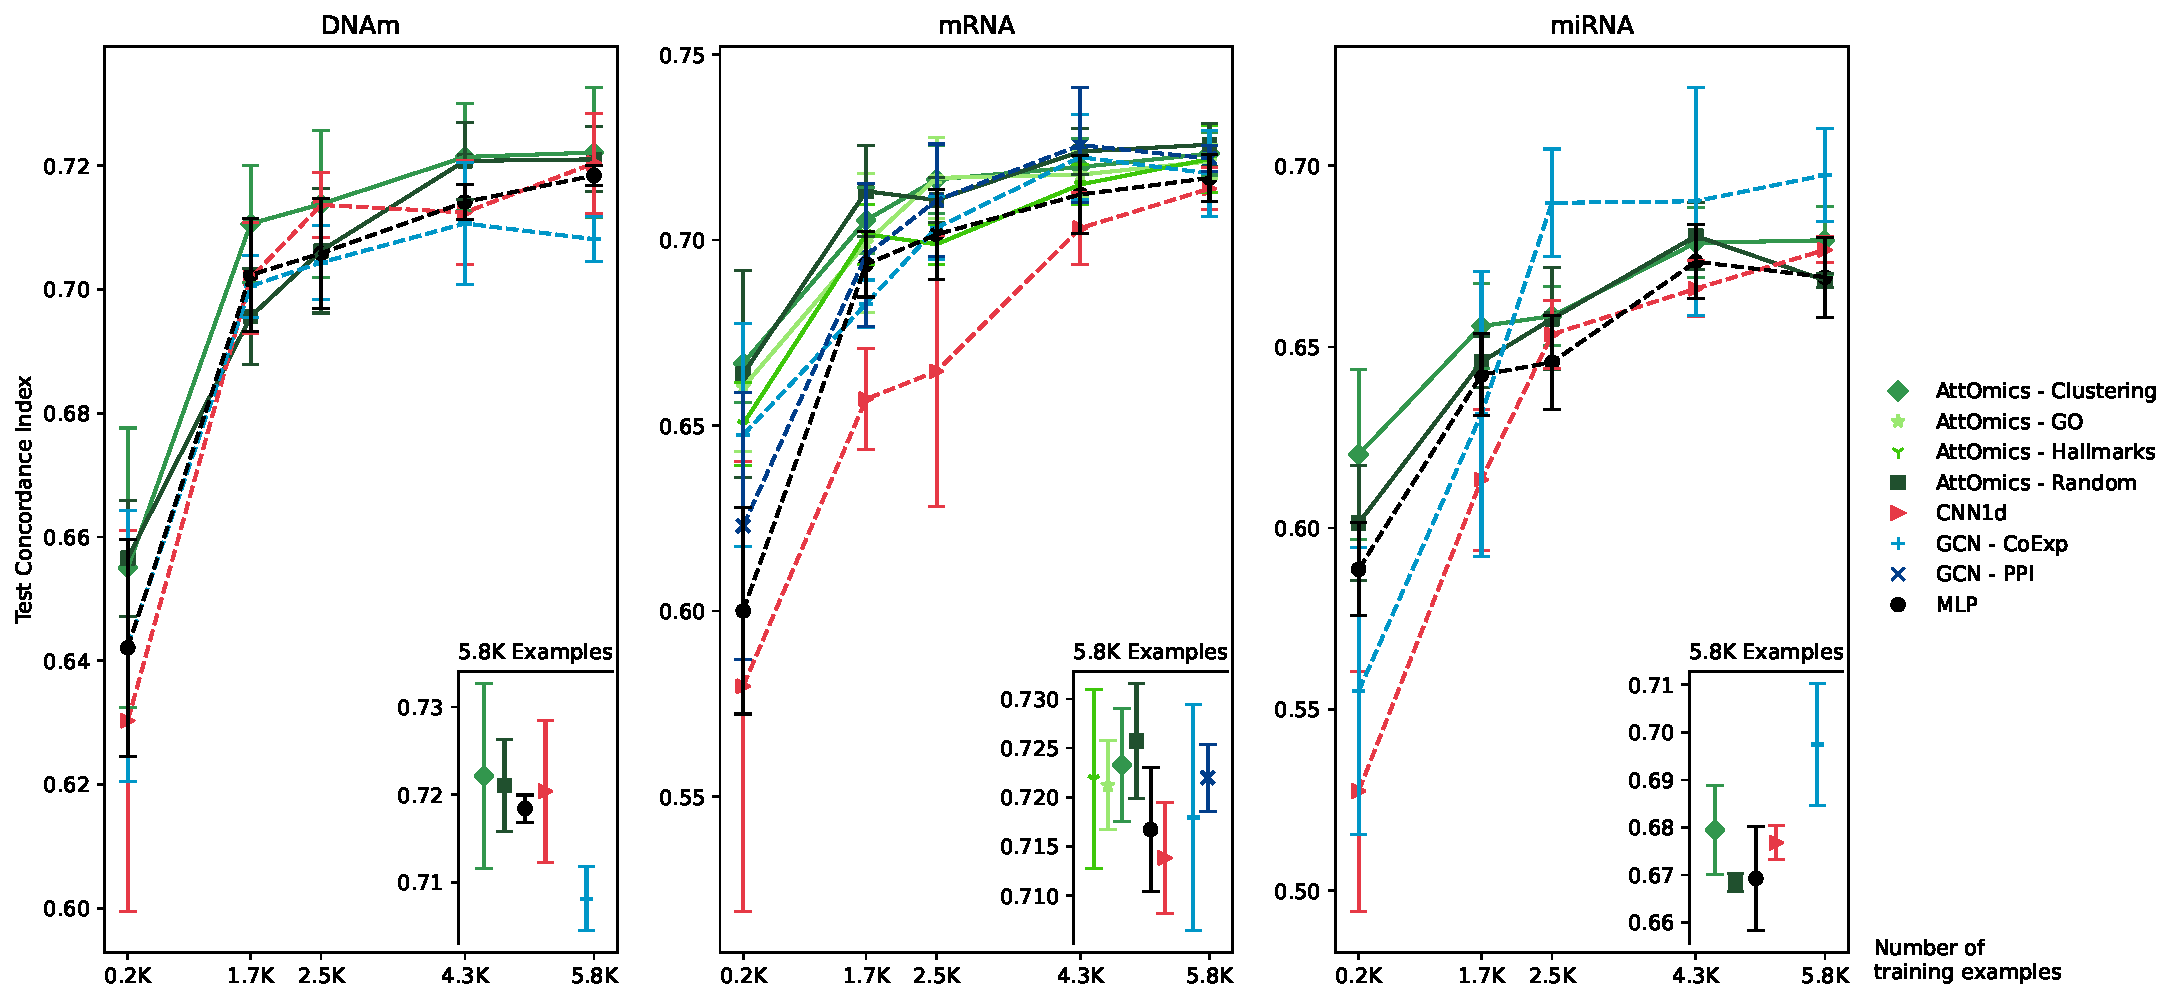
\includegraphics[width=0.9\textwidth]{cancer_type_limited_training_survival.pdf}
	\caption{Concordance Index on the test set according to the size of the training set. }\label{fig:limit_train_cox}
\end{figure}

\begin{table}[htbp]
	\centering
	\caption{Comparison of the time required to obtain predictions from the different models on the test set. }\label{tab:arch_timings}
	\begin{tblr}{
		colspec={
				Q[l,m]
				Q[l,m]
				Q[r,m]
			},%
		row{1} = {guard, c},%
		row{2-Z} = {font=\small},%
		hline{1,Z} = {2pt},%
		hline{2} = {1pt},%
		hline{10,21} = {1pt, dashed},
				cell{2}{1} = {r=8,c=1}{l,m},
				cell{10}{1} = {r=11,c=1}{l,m},
				cell{21}{1} = {r=8,c=1}{l,m},
			}
		Omics & Model                 & Time (s) \\
		DNAm  & AttOmics – Clustering & 0.006    \\
		      & AttOmics – Random     & 0.004    \\
		      & CNN1d                 & 0.078    \\
		      & GNN – CoExp           & 6.280    \\
		      & MLP                   & 0.001    \\
		      & RF                    & 0.046    \\
		      & SVM                   & 5.914    \\
		      & XGBoost               & 0.019    \\
		mRNA  & AttOmics – Clustering & 0.008    \\
		      & AttOmics – GO         & 0.028    \\
		      & AttOmics – Hallmarks  & 0.005    \\
		      & AttOmics – Random     & 0.008    \\
		      & CNN1d                 & 0.178    \\
		      & GNN – CoExp           & 6.623    \\
		      & GNN – PPI             & 2.564    \\
		      & MLP                   & 0.010    \\
		      & RF                    & 0.040    \\
		      & SVM                   & 12.850   \\
		      & XGBoost               & 0.028    \\
		miRNA & AttOmics – Clustering & 0.002    \\
		      & AttOmics – Random     & 0.002    \\
		      & CNN1d                 & 0.006    \\
		      & GNN – CoExp           & 0.326    \\
		      & MLP                   & 0.001    \\
		      & RF                    & 0.270    \\
		      & SVM                   & 20.868   \\
		      & XGBoost               & 0.022    \\
	\end{tblr}
\end{table}

\begin{figure}[htbp]
	\centering
	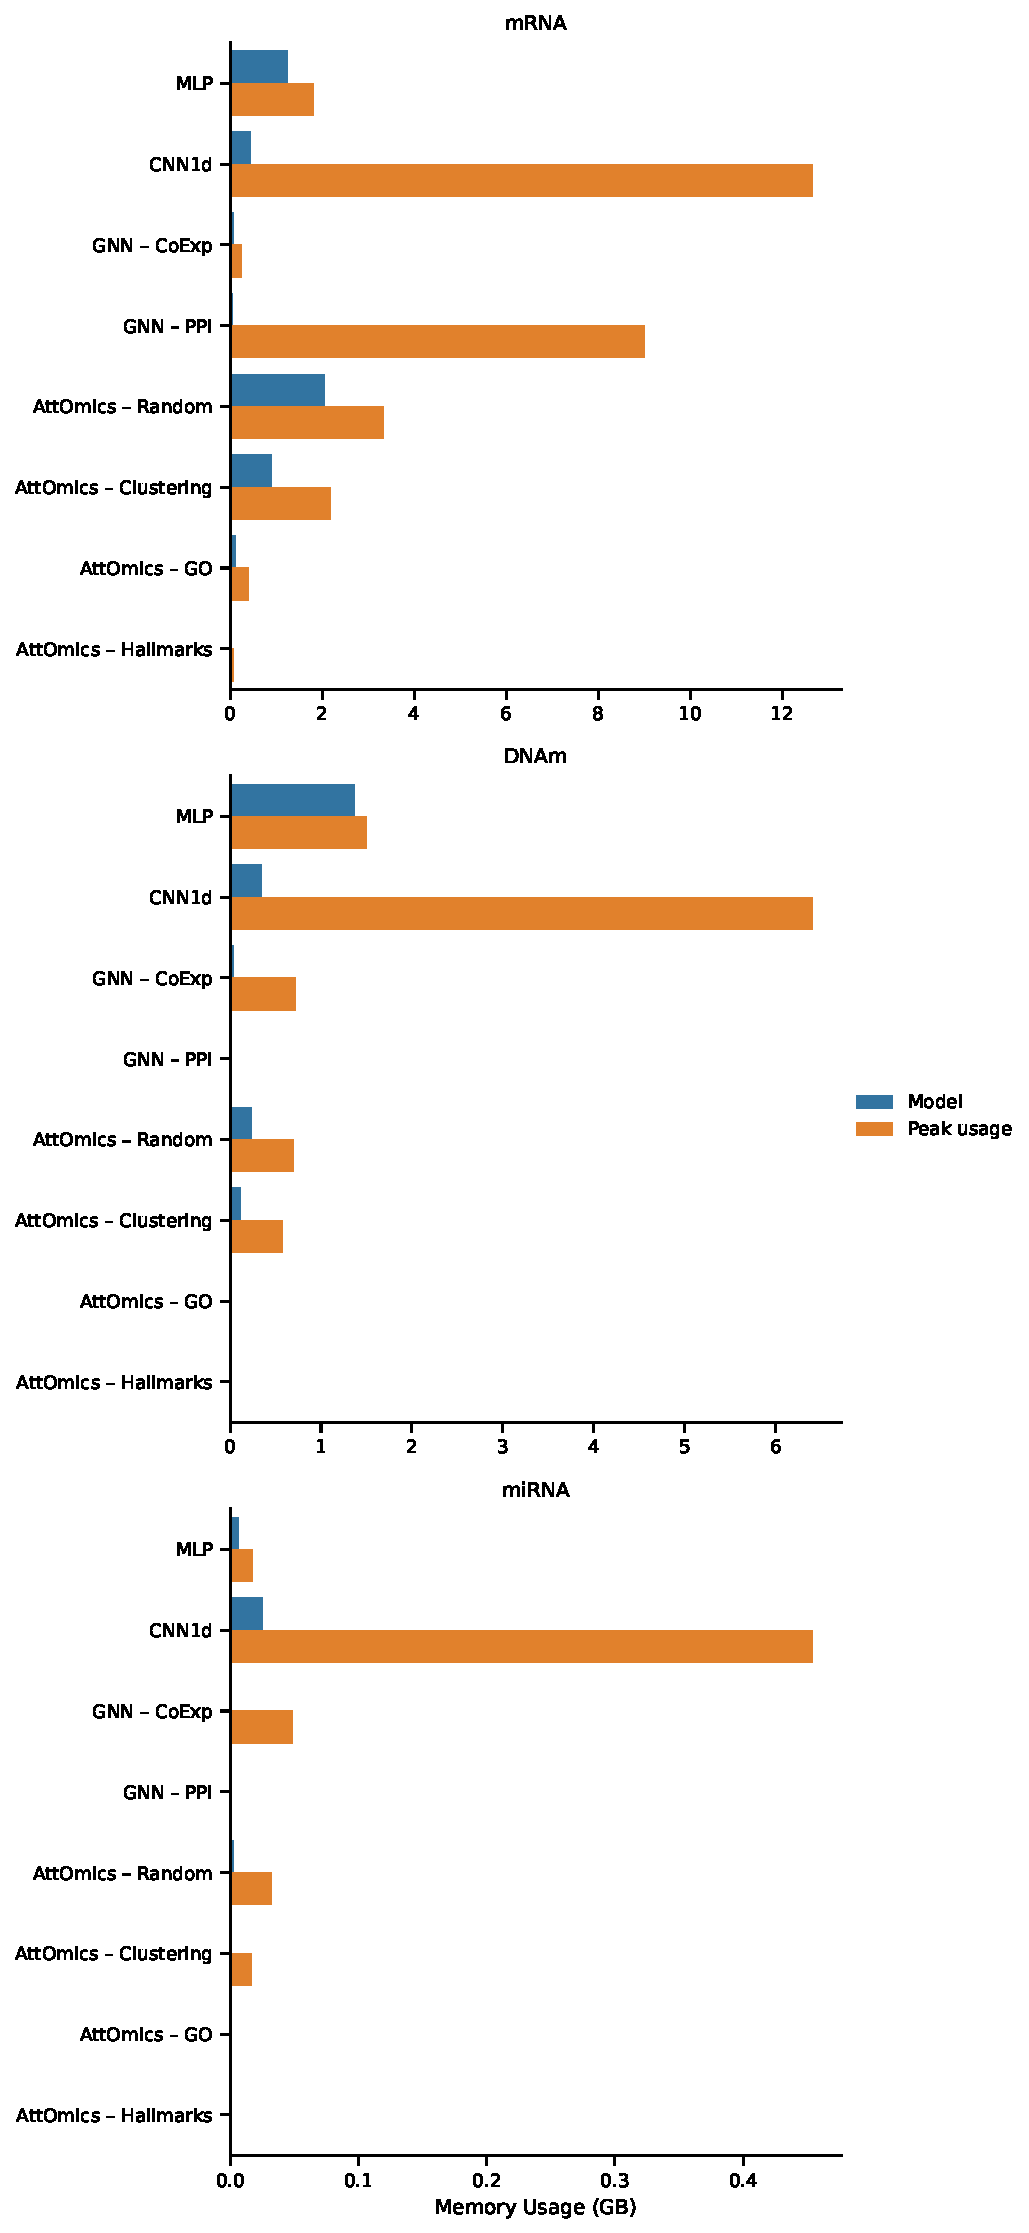
\includegraphics[scale=0.5]{memory_usage_models.pdf}
	\caption{Comparison of the memory usage of the different deep-learning models and the peak of memory usage during inference on the test set.}\label{fig:mem_uasge}
\end{figure}



\begin{figure}[htbp]
	\centering
	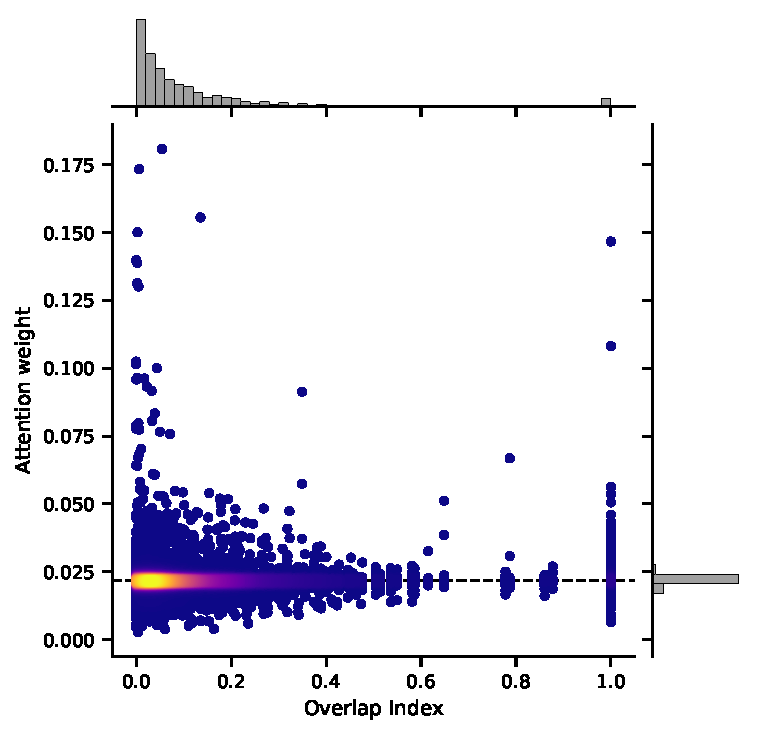
\includegraphics[width=\textwidth]{attention_weight_overlap.pdf}
	\caption{Attention weight and overlap index comparison for grouped based on GO\@. The dashed line correspond to the expected mean attention weight (\(\frac{1}{n_{groups}} \)). Points are colored based on the density of points.}\label{fig:att_w_overlap}
\end{figure}

\begin{landscape}
	\begin{figure}[p]
		\centering
		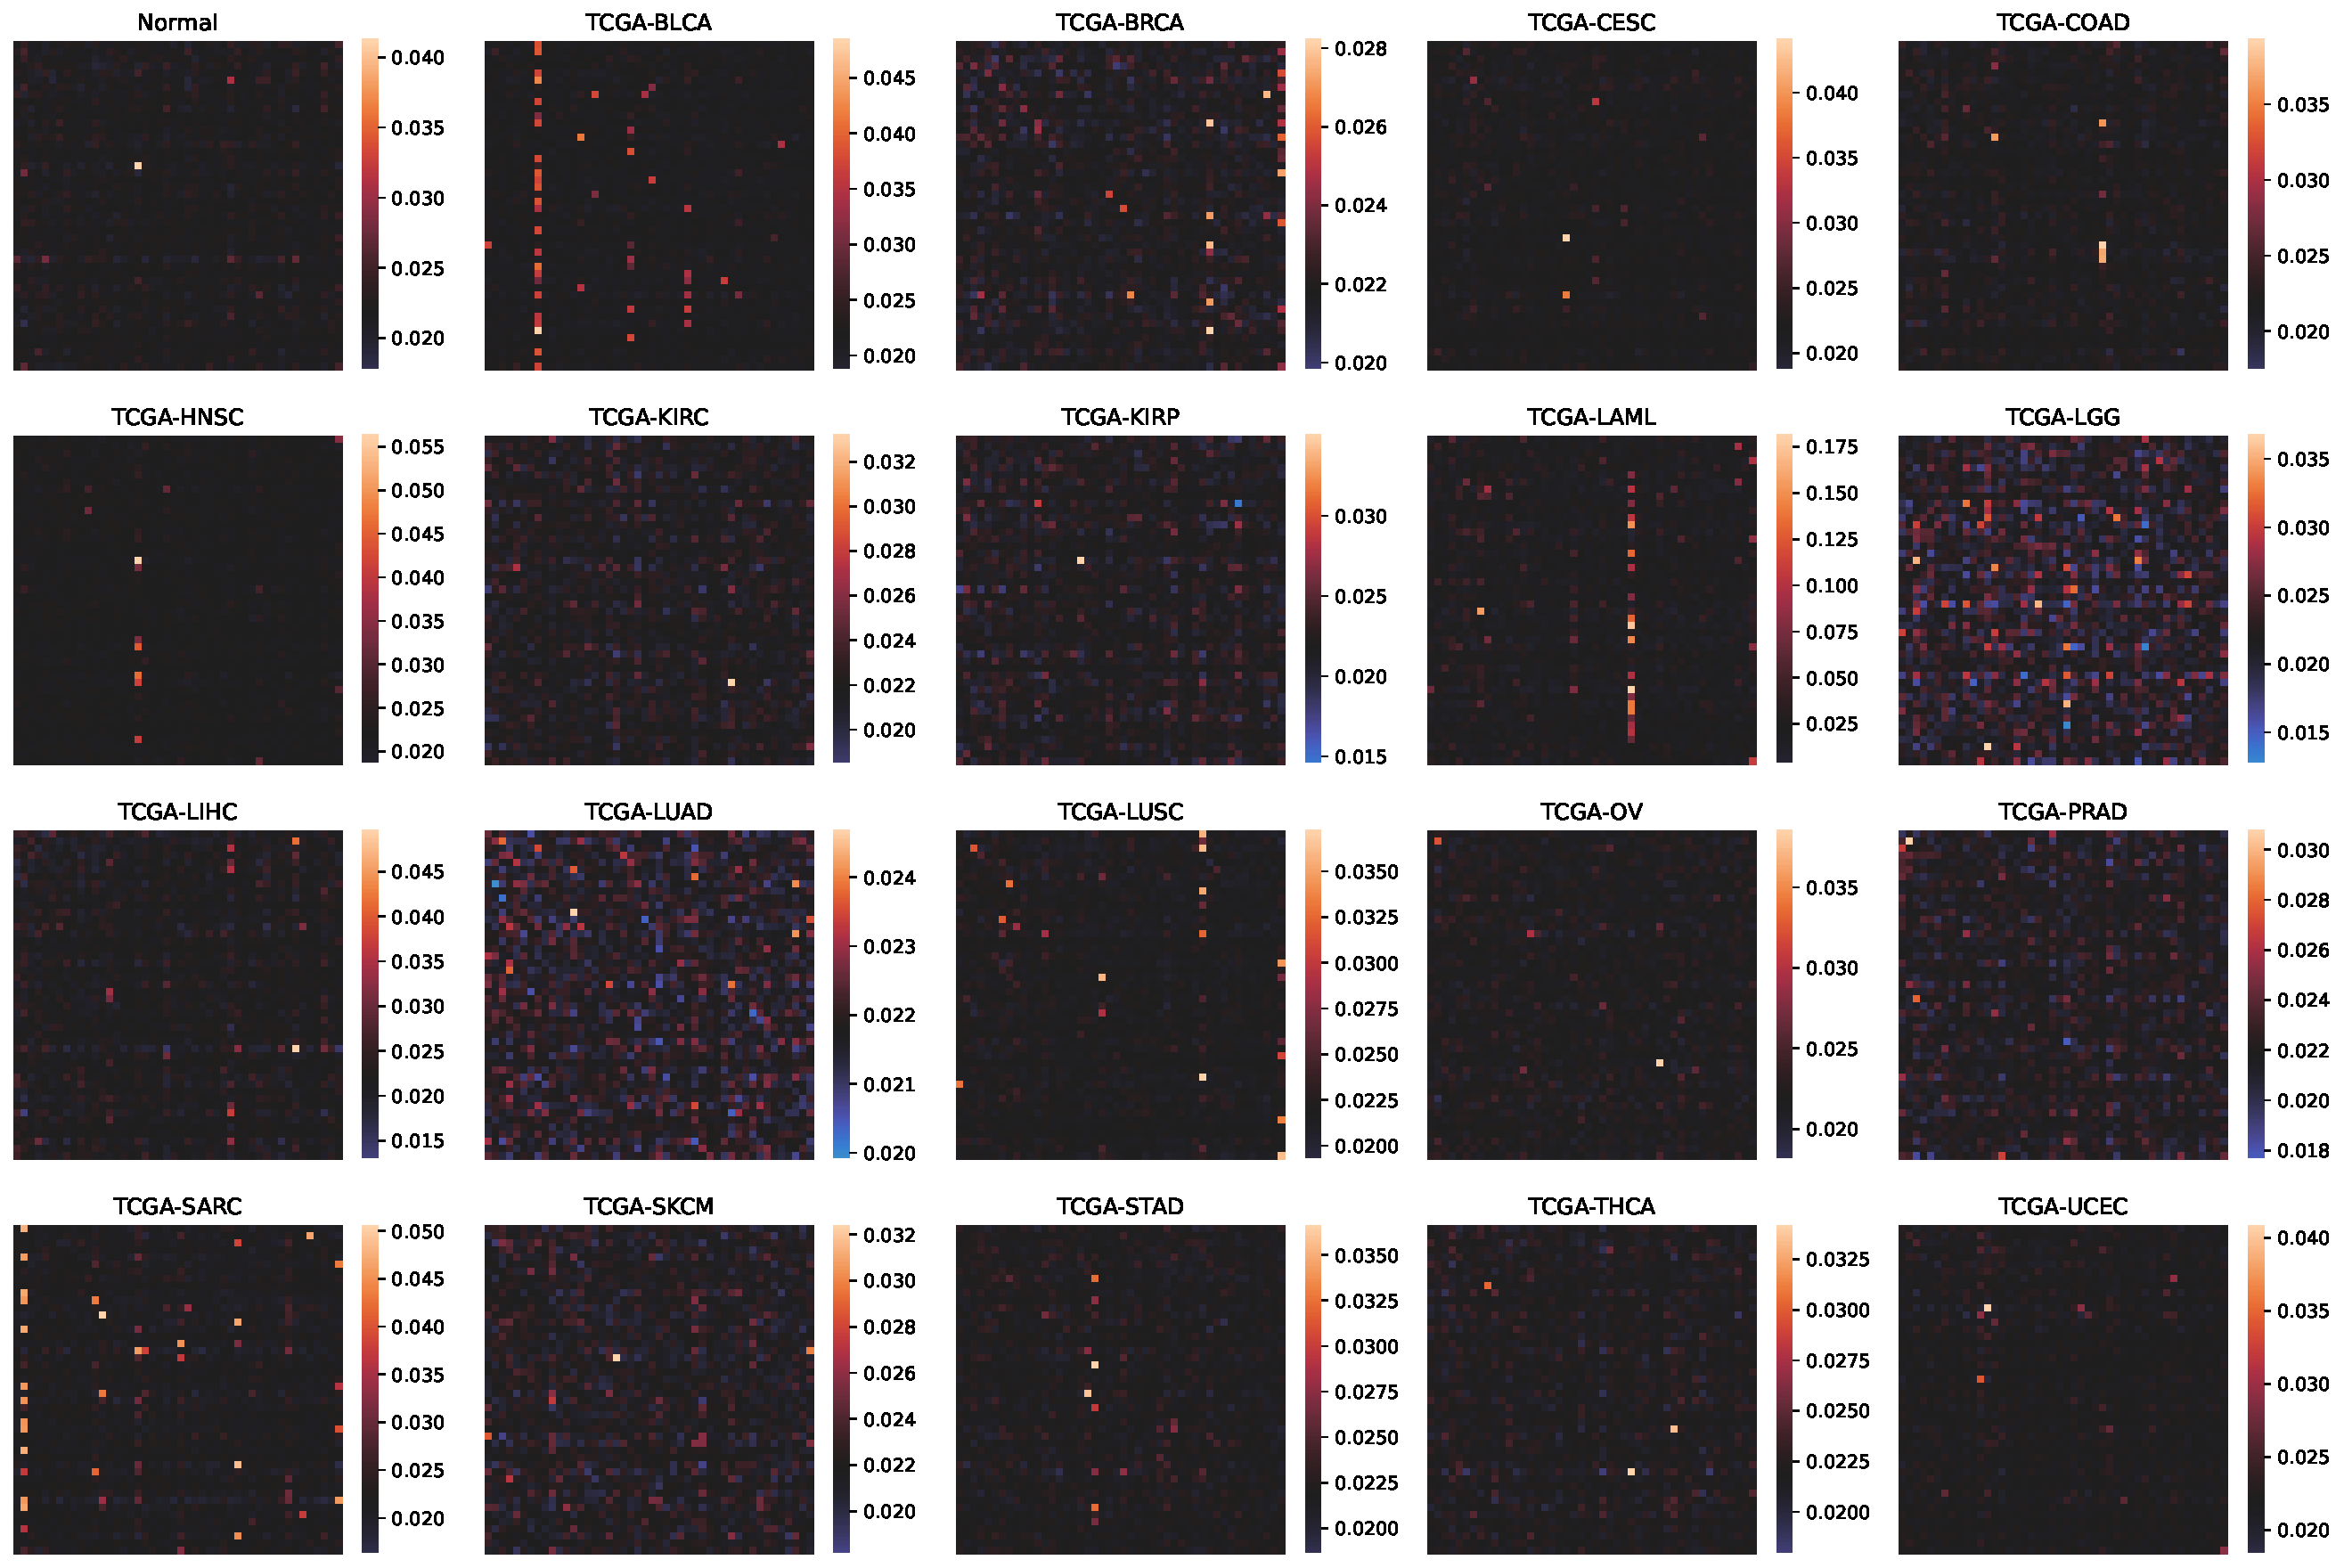
\includegraphics[width=0.9\textheight]{attention_maps_cancer_go_block1.pdf}
		\caption{Attention map visualized per cancer for the first block when grouping with the gene ontology strategy. Attention map per cancer are obtained by taking the mean of the attention map of all patients with the corresponding cancer. }\label{fig:att_map_cancer_go}
	\end{figure}

	\begin{figure}[p]
		\centering
		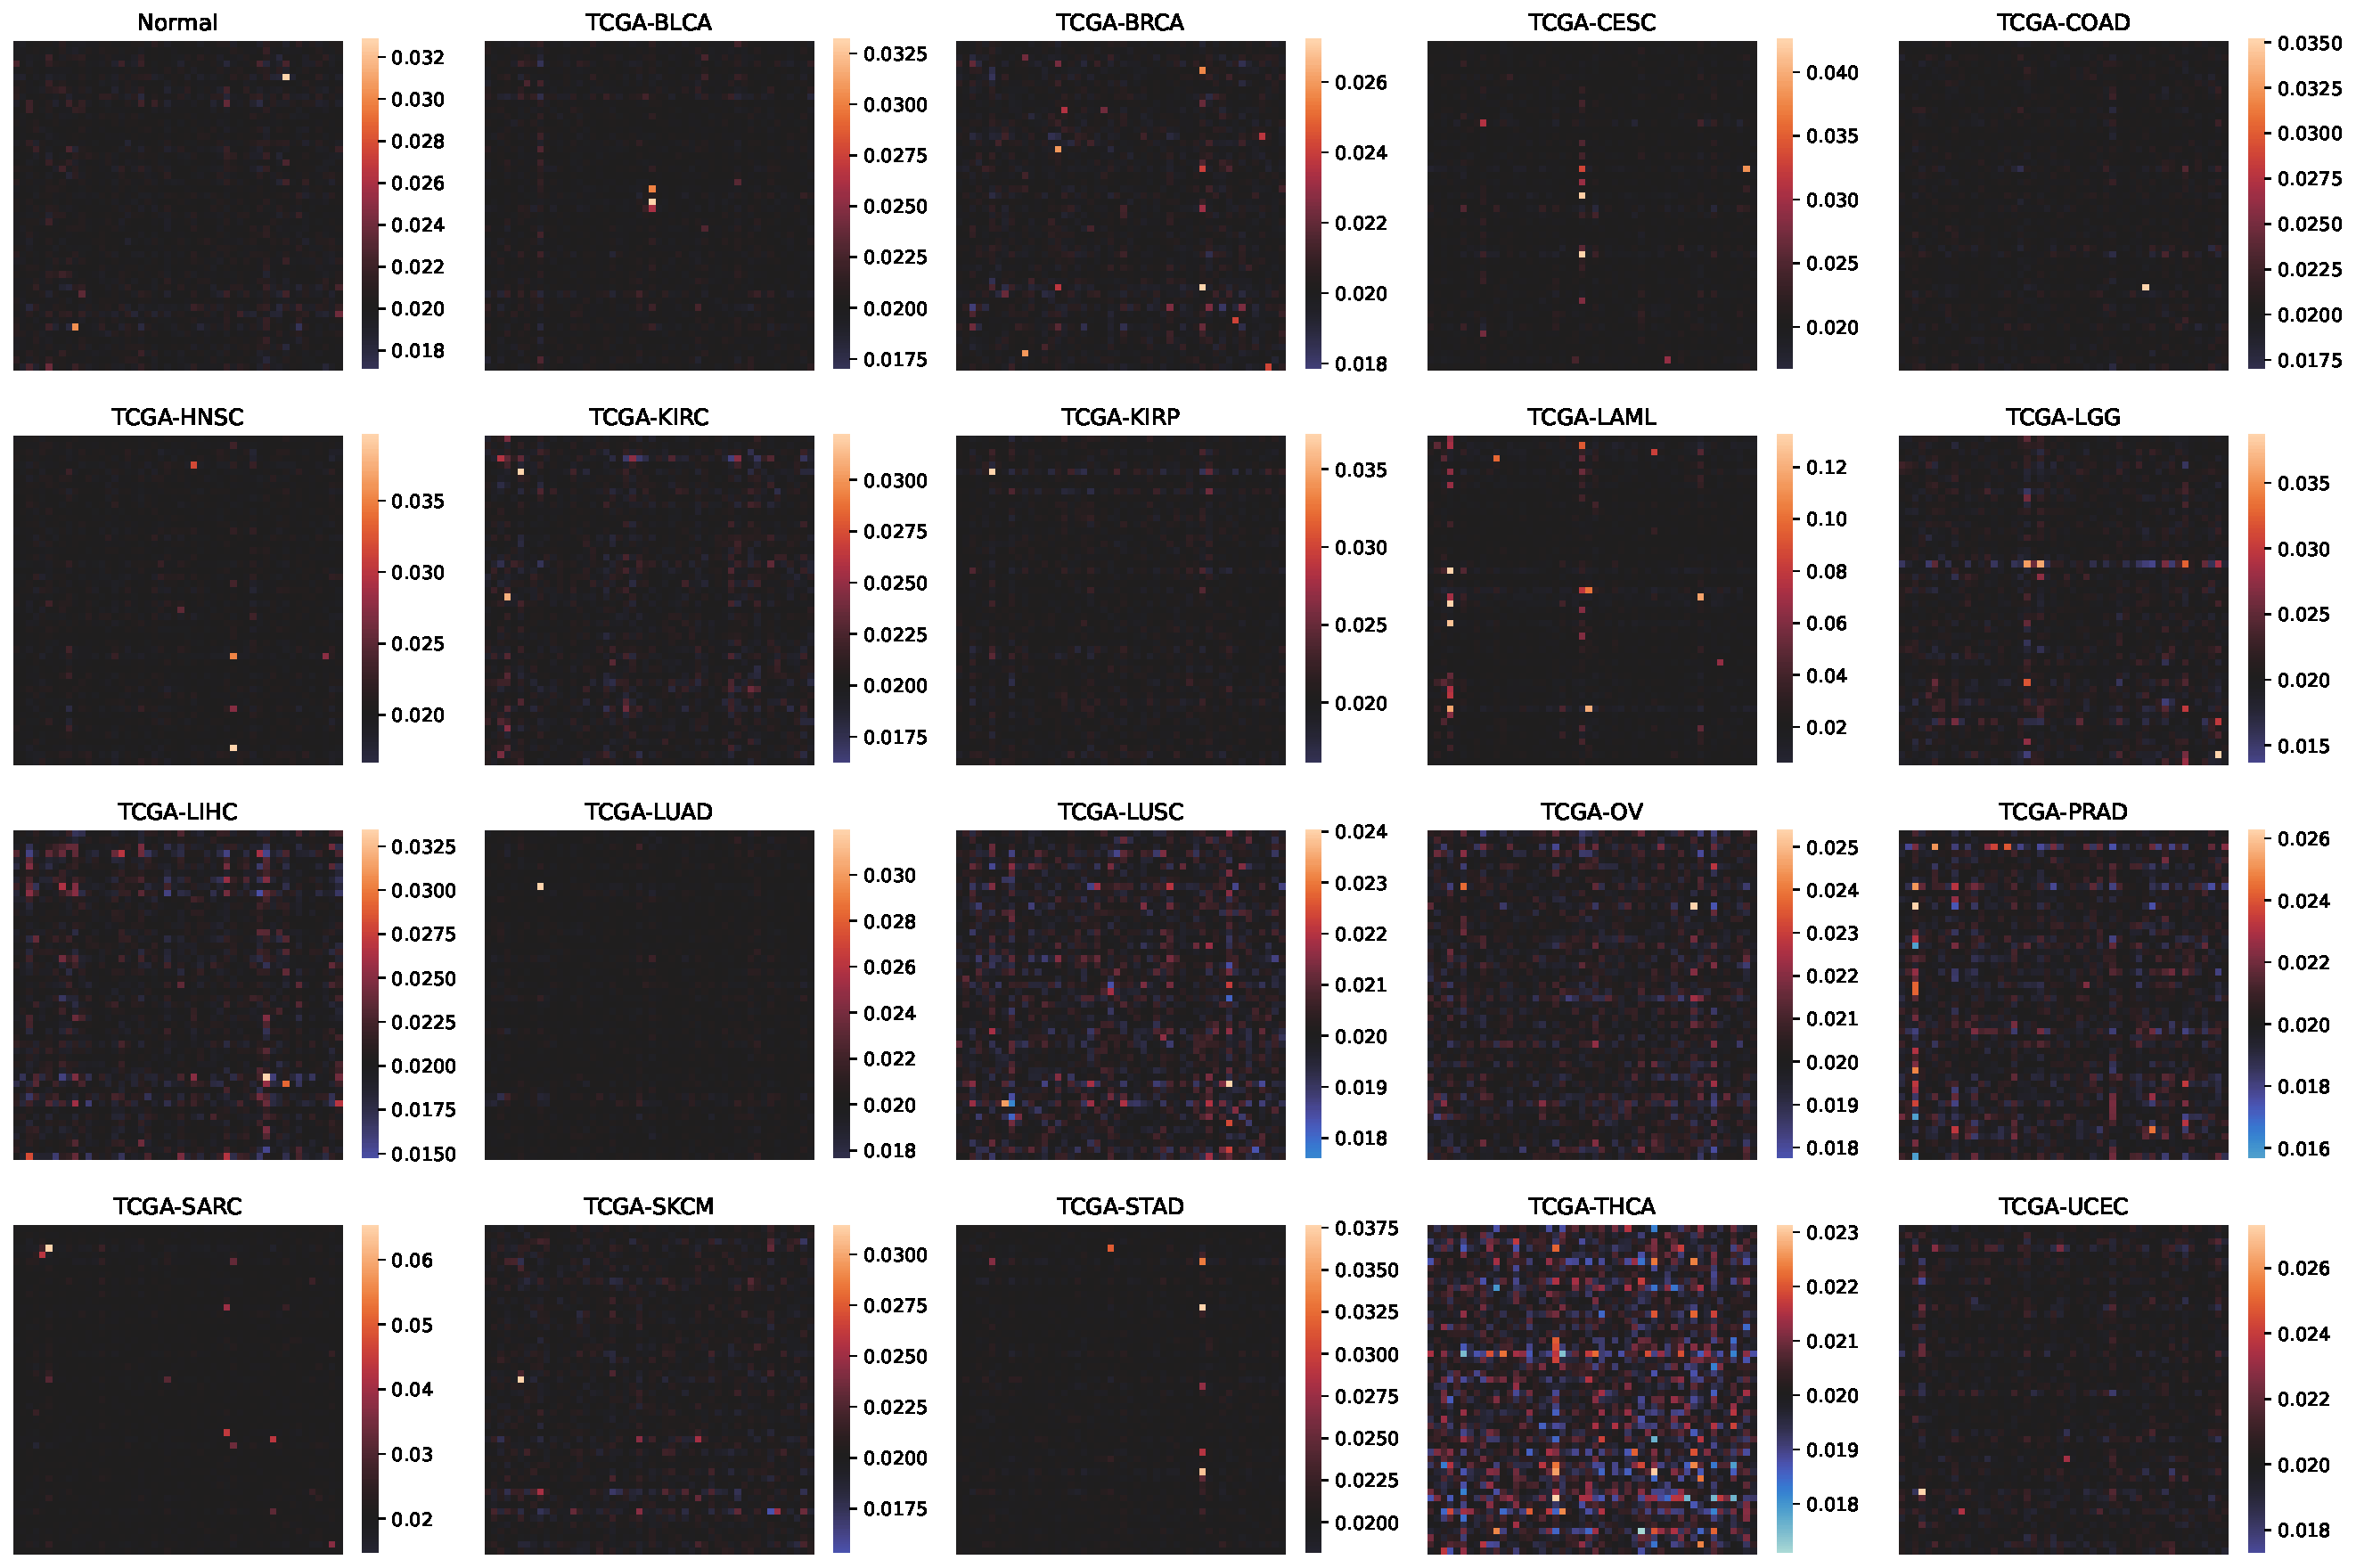
\includegraphics[width=0.9\textheight]{attention_maps_cancer_hallmarks_block1.pdf}
		\caption{Attention map visualized per cancer for the first block when grouping with the hallmarks strategy. Attention map per cancer are obtained by taking the mean of the attention map of all patients with the corresponding cancer. }\label{fig:att_map_cancer_hallmarks}
	\end{figure}

	\begin{figure}[p]
		\centering
		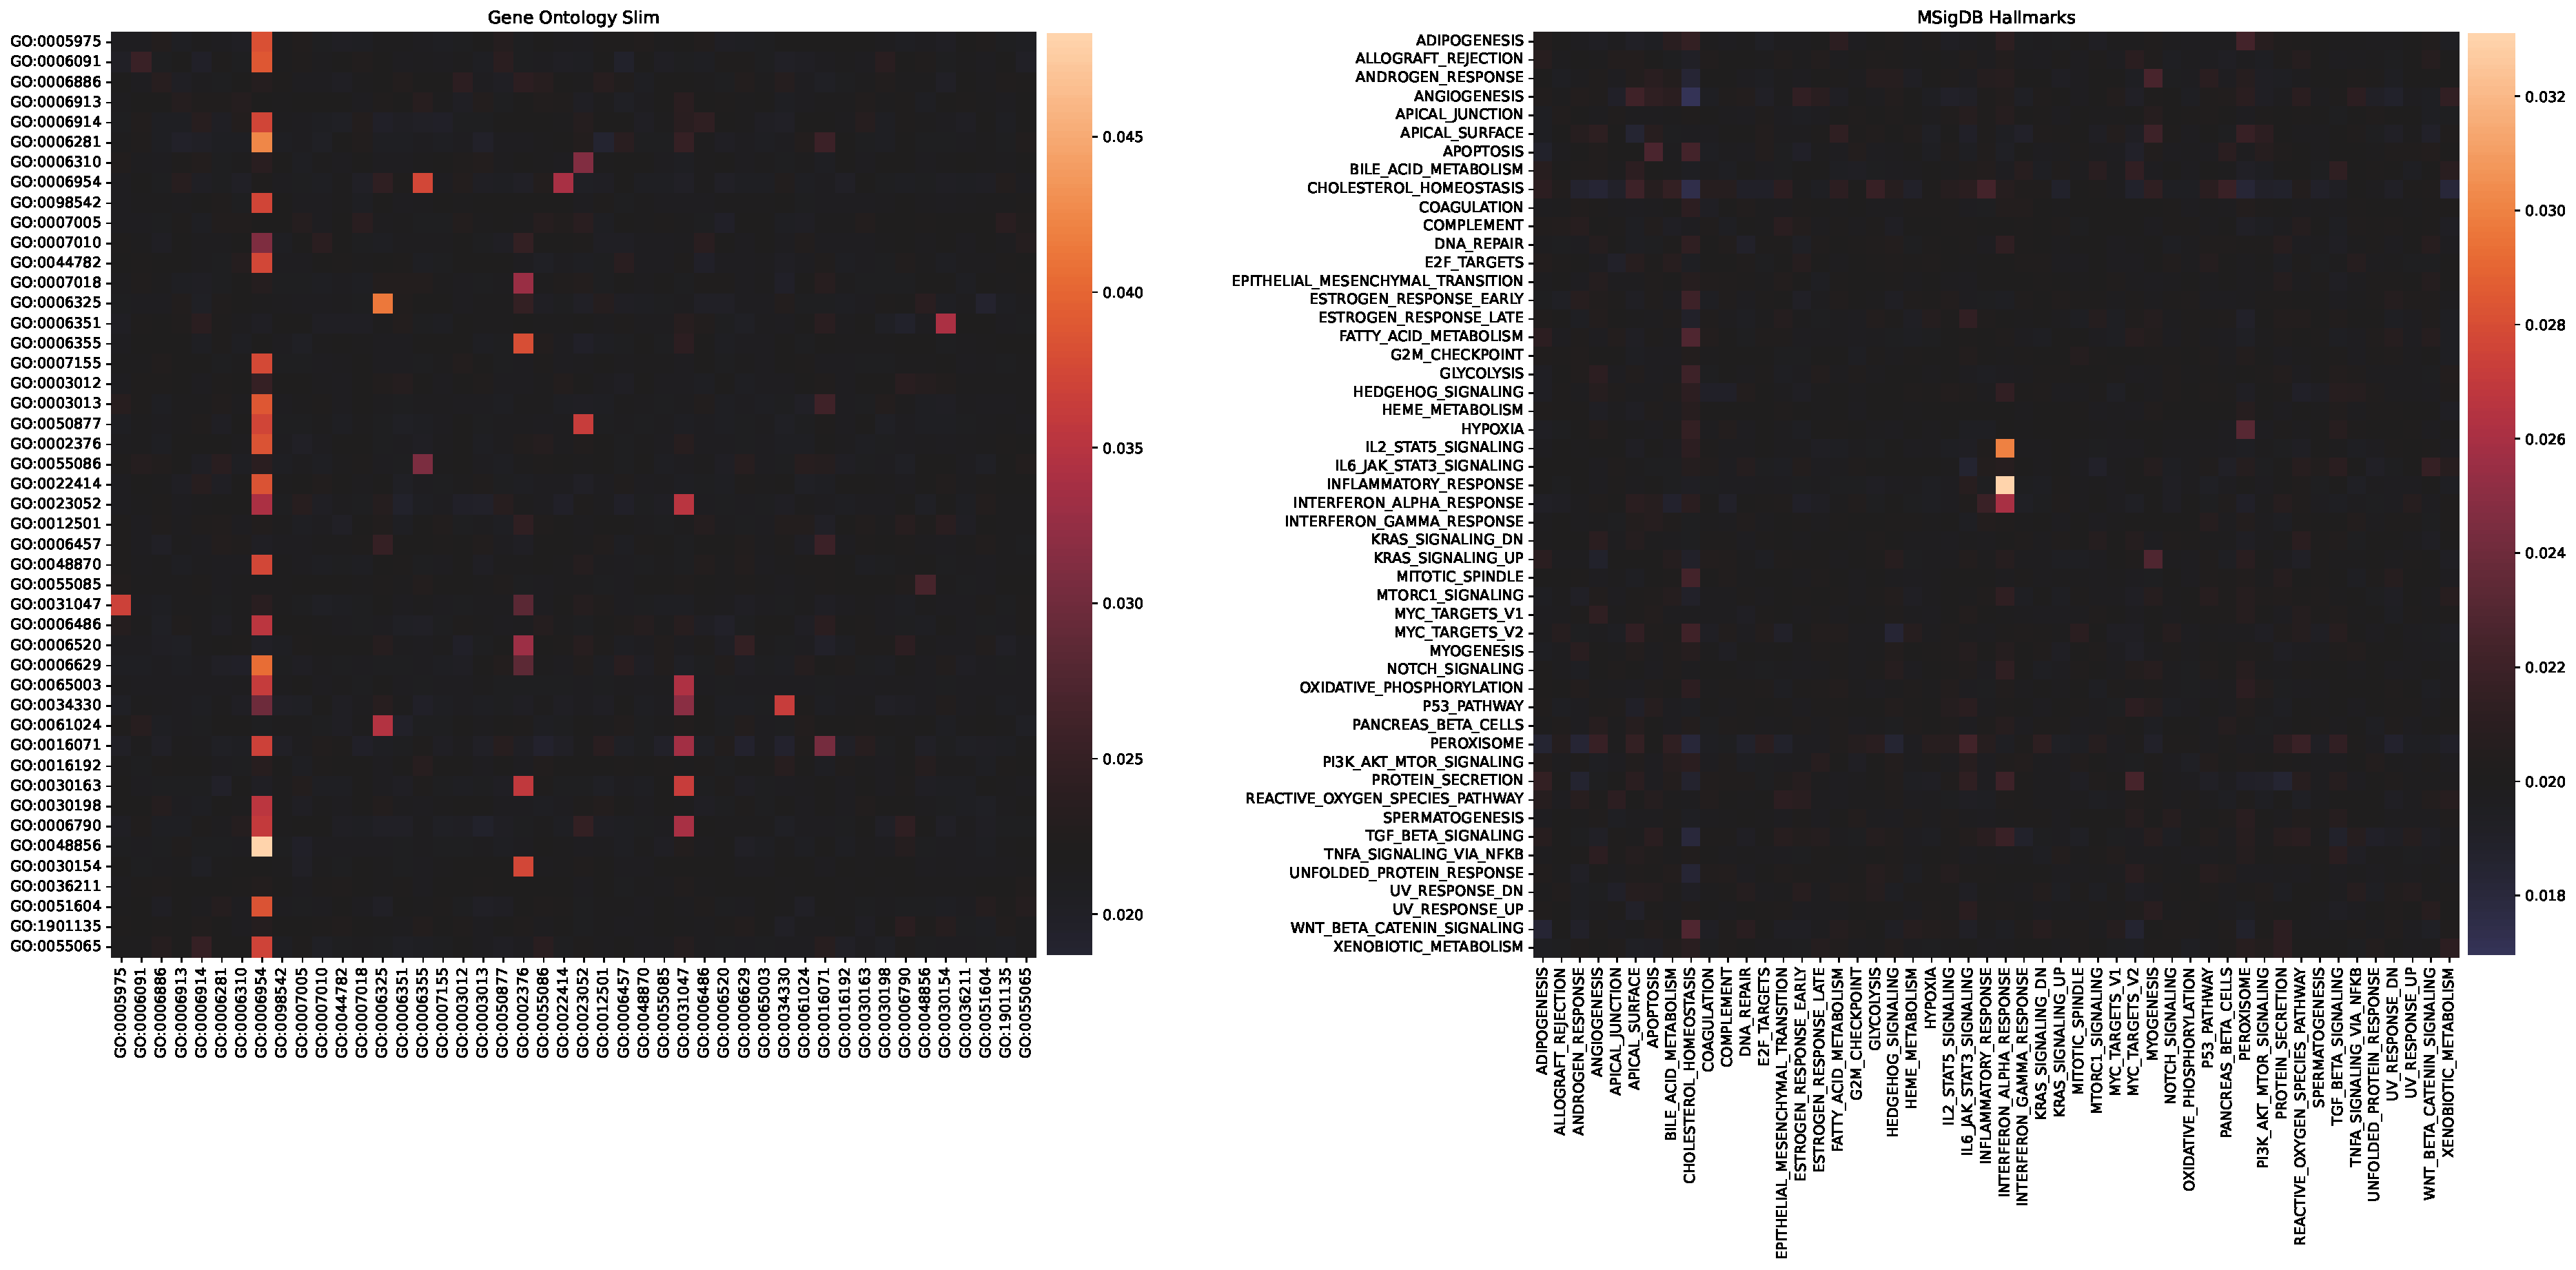
\includegraphics[width=0.9\textheight]{TCGA_BLCA_comparison_attention_go_hallmarks.pdf}
		\caption{Comparison of the attention maps obtained with the gene ontology and the hallmarks grouping strategy. Both attention map highlights interaction involving an inflammatory response group. }\label{fig:att_map_blca_comp}
	\end{figure}
\end{landscape}
\chapter{CrossAttOmics supplementary}

\section{Experiments}

 \subsection{Architecture and training details}
     For a comprehensive and comparative evaluation, we chose various deep learning architectures with different integration strategies: \gls{mlp} early fusion (MLP EF), \gls{mlp} intermediate fusion (MLP IF), AttOmics early fusion (AttOmics EF), AttOmics intermediate fusion (AttOmics IF), \gls{gnn} early fusion (GNN EF), P-NET and MOGONET.
     We also considered single-omics architecture for comparison: attention-based model~(AttOmics), \gls{mlp} and \gls{gnn}.

     The \gls{mlp} is based on a \gls{fcn} with \gls{relu} activations.
     For the \gls{mlp} EF architecture, input modalities are concatenanted before being passed to a \gls{mlp}.
     For the \gls{mlp} IF architecture, the modalities encoders were constructed similarly to the unimodal \gls{mlp} architecture described previously.
     Unimodal latent representations are concatenated and passed to a 2-layers \gls{fcn} with \gls{relu} activations.

     AttOmics is an attention-based architecture.
     Input is randomly split in groups, then each group in embed in a latent space with a group-specific \gls{fcn}.
     Groups are enriched with information from other groups with \gls{mhsa}.
     For the AttOmics IF architecture, the modalities encoders were constructed similarly to the unimodal AttOmics architecture described previously.
     Unimodal latent representations are concatenated and passed to a 3-layers \gls{fcn} with \gls{relu} activations.

     For the \gls{gnn} architecture the \gls{ppi} graph is based on data available in the STRING database and was constructed by retaining only high-confidence links: edges with a score higher than 700.
     We used graph convolutions described in Kipf et al., with a single input and output channel for unimodal training.
     All the nodes are concatenated and passed to a 2-layers \gls{fcn} with a \gls{relu} activation.
     For the \gls{gnn} EF, the number of channels was set to the number of modalities used for the training.

     In all the architectures the output layer has a \(\operatorname{softmax}\) activation.

     CrossAttOmics is trained using the SGD optimizer with a learning rate of 0.001, a momentum of 0.9, and a batch size of 512.
     Our 2-phase training allows us to train each encoder with more training examples.
     An ablation study showed that the \gls{mhsa} after concatenating the cross-attention outputs was not necessary.
     When creating the different splits, we paid attention to not including examples used in the pre-training phase in our final test set.
     The maximum number of epochs is set to 200.
     An early stopping strategy is deployed to avoid over-fitting with a patience of 10 and a delta of 0.001 on the validation loss between two epochs.
     Models were evaluated with the accuracy metric; other classification metrics are available in the supplementary file.
     All models were trained on an Nvidia GeForce RTX 3090.

     ~\\
     Thomas N. Kipf, and Max Welling. Semi-Supervised Classification with Graph Convolutional Networks. In \textit{5th International Conference on Learning Representations, ICLR} 2017.

     \newpage
\section{Supplementary figures}

 \begin{table}[htbp]
     \centering
     \caption{Distribution of the samples across cancer and splits for (\subref{tab:tcga}) TCGA and (\subref{tab:ccle}) CCLE.}
     \begin{subtable}[t]{0.45\textwidth}
         \subcaption{}
         \begin{tabular}{lrrrr}
             \toprule
             Cancer & Train & Validation & Test & Total \\
             \midrule
             BLCA   & 222   & 48         & 48   & 318   \\
             BRCA   & 574   & 123        & 124  & 821   \\
             CESC   & 113   & 24         & 25   & 162   \\
             COAD   & 230   & 50         & 50   & 330   \\
             HNSC   & 228   & 49         & 49   & 326   \\
             KIRC   & 171   & 37         & 37   & 245   \\
             KIRP   & 145   & 31         & 32   & 208   \\
             LGG    & 296   & 64         & 64   & 424   \\
             LIHC   & 118   & 25         & 26   & 169   \\
             LUAD   & 238   & 51         & 52   & 341   \\
             LUSC   & 205   & 44         & 44   & 293   \\
             OV     & 182   & 39         & 39   & 260   \\
             PRAD   & 234   & 50         & 51   & 335   \\
             SARC   & 143   & 31         & 31   & 205   \\
             SKCM   & 227   & 49         & 49   & 325   \\
             STAD   & 226   & 49         & 49   & 324   \\
             THCA   & 254   & 55         & 55   & 364   \\
             UCEC   & 288   & 62         & 62   & 412   \\
             \midrule
             Total  & 4094  & 881        & 887  & 5862  \\
             \bottomrule
         \end{tabular}
         \label{tab:tcga}
     \end{subtable}
     \begin{subtable}[t]{0.45\textwidth}
         \subcaption{}
         \begin{tabular}{lrrrr}
             \toprule
             Cancer    & Train & Validation & Test & Total \\
             \midrule
             ALL       & 16    & 4          & 4    & 24    \\
             BRCA      & 29    & 6          & 7    & 42    \\
             COAD-READ & 32    & 7          & 7    & 46    \\
             DLBC      & 23    & 5          & 6    & 34    \\
             GBM       & 19    & 4          & 5    & 28    \\
             HNSC      & 20    & 4          & 5    & 29    \\
             KIRC      & 12    & 3          & 3    & 18    \\
             LAML      & 19    & 4          & 5    & 28    \\
             LUAD      & 39    & 8          & 9    & 56    \\
             MM        & 11    & 2          & 3    & 16    \\
             OV        & 25    & 6          & 6    & 37    \\
             PAAD      & 23    & 5          & 5    & 33    \\
             SARC      & 16    & 4          & 4    & 24    \\
             SCLC      & 30    & 6          & 7    & 43    \\
             SKCM      & 32    & 7          & 7    & 46    \\
             STAD      & 22    & 5          & 5    & 32    \\
             \midrule
             Total     & 368   & 80         & 88   & 536   \\
             \bottomrule
         \end{tabular}
         \label{tab:ccle}
     \end{subtable}
 \end{table}

 \begin{figure}
     \centering
     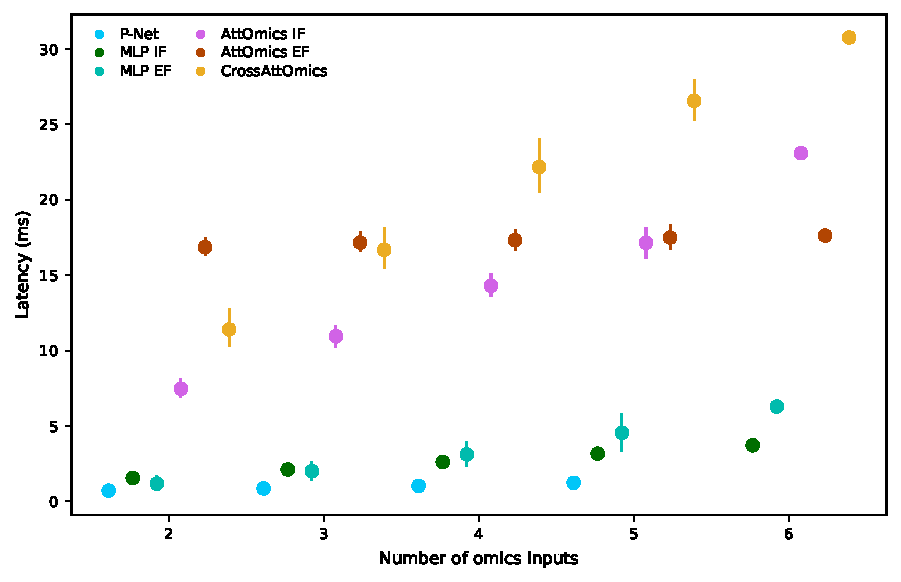
\includegraphics[width=\linewidth]{multi_omics_latency.pdf}
     \caption{Comparison of the latency, or time in milliseconds to get a prediction for one sample with various number of input omics. Error-bars represent latency variation across the various possible omics combinations.}
     \label{fig:latency}
 \end{figure}

 \begin{figure}[htbp]
     \centering
     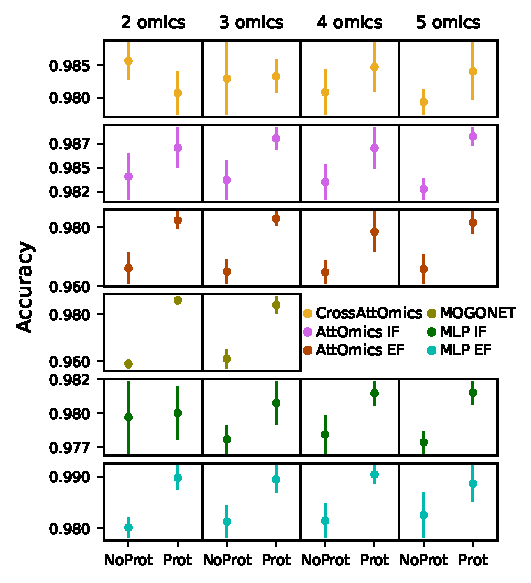
\includegraphics{perf_gain_prot.pdf}
     \caption{Impact of proteins on the test accuracy when training CrossAttOmics with a fixed number of omics on the TCGA dataset.}
     \label{fig:perf_gain_prot}
 \end{figure}

 \begin{figure}[htbp]
     \centering
     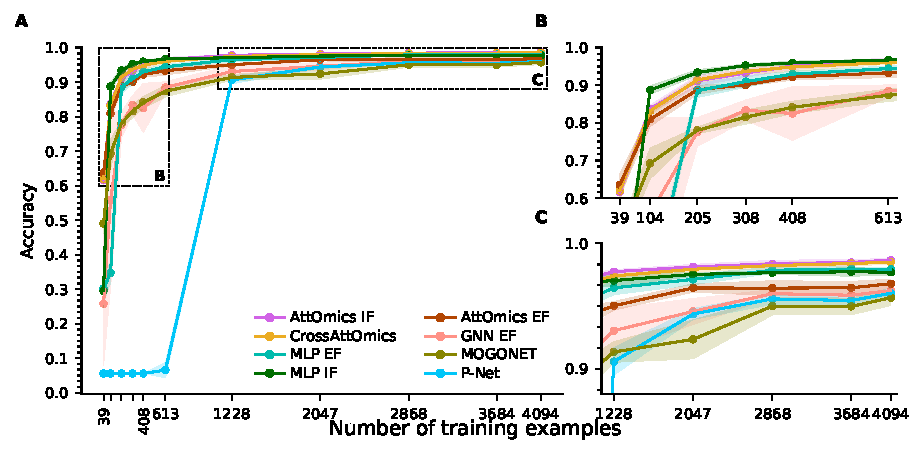
\includegraphics{limited_training_3_omics.pdf}
     \caption{Accuracy on the TCGA test set according to the size of the training set for various multi-omics deep learning models when trained on the best combination of 3 omics. When trained with the minimum samples possible, CrossAttOmics outperformed MLP IF. When the number of training samples was increased, MLP IF became the better architecture. The performance of CrossAttOmics depends on the number of modalities used, which impacts the number of cross-attentions. With the selected omics, miRNA, nc mRNA, and DNAm~(Figure~\ref{fig:tcga_perf_comb}), there is only two cross-attention to compute. The model cannot benefit from the cross-attention mechanism compared to situations with more modalities~(Figure~\ref{fig:lim_train_6_omics}).}
     \label{fig:lim_train_3_omics}
 \end{figure}



 \begin{figure}[htbp]
     \centering
     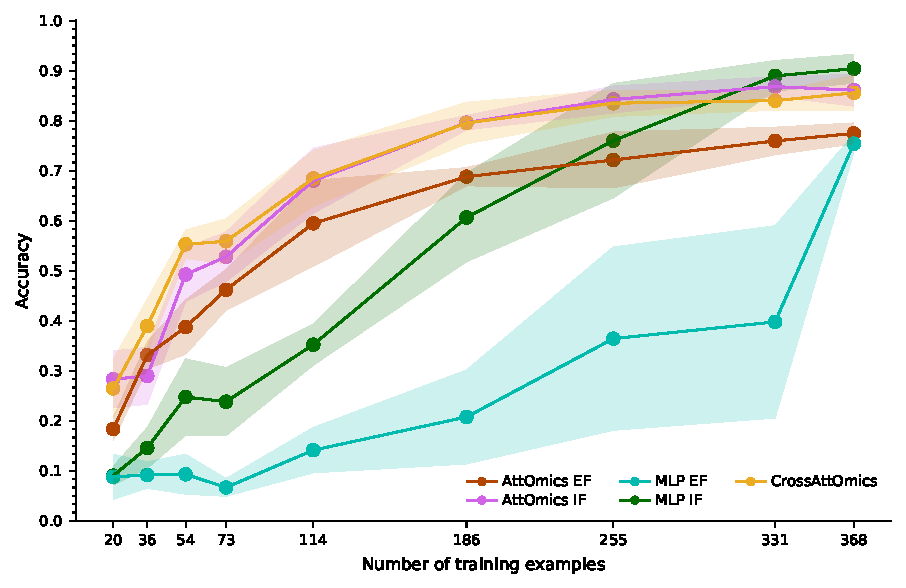
\includegraphics{ccle_limited_training_3_omics.pdf}
     \caption{Accuracy on the CCLE test set according to the size of the training set for various multi-omics deep learning models when trained on the best combination of 3 omics.}
     \label{fig:ccle_limited_train}
 \end{figure}

 \begin{figure}[htbp]
     \centering
     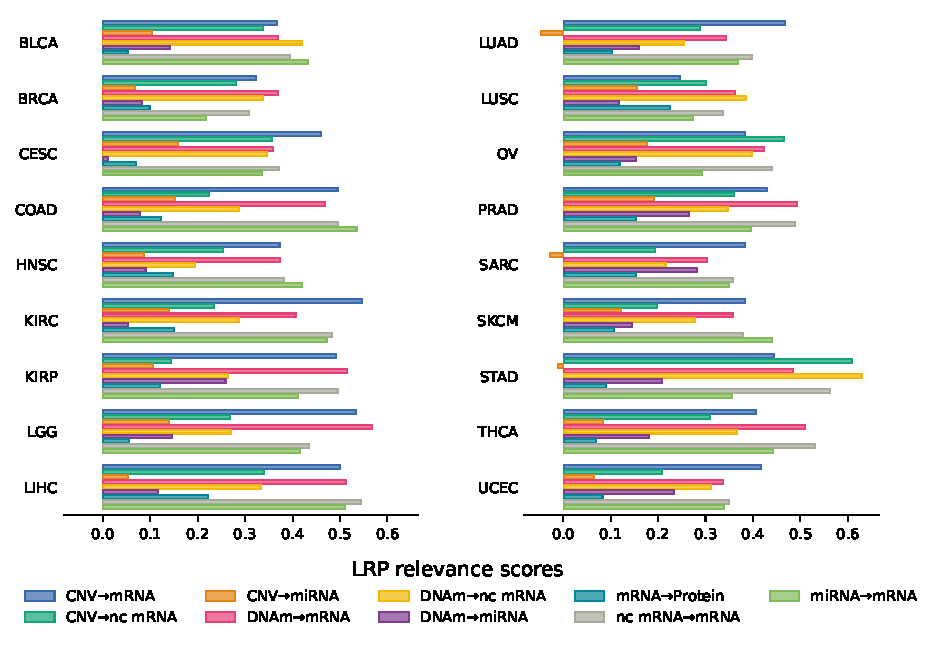
\includegraphics{LRP_crossattomics.pdf}
     \caption{Comparison of the LRP relevance score for the different modelled modality interactions across various cancer.}
     \label{fig:LRP_CrossAttOmics}
 \end{figure}

 \begin{figure}[htbp]
     \centering
     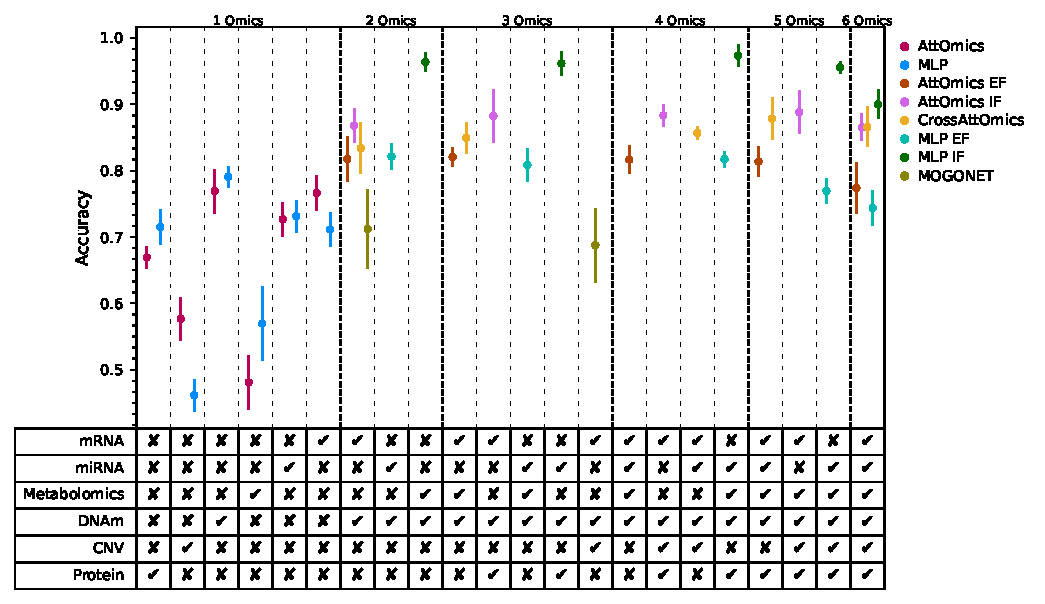
\includegraphics[width=1\textwidth]{ccle_omics_com.pdf}
     \caption{Comparison of the test accuracy of different multi-omics deep learning integration models across different omics combination on the CCLE dataset. Each dot represents the mean accuracy obtained by a model on the test set after 5 different training. The error-bars represents the standard-error. For each combination a \cmark means that the omics is included in the combination and a \xmark means that the omics is excluded from the combination.}
     \label{fig:ccle_perf_comb}
 \end{figure}

 \begin{landscape}
     \section{Supplementary tables}
      \subsection{Models performances on various combinations of omics on TCGA dataset}
          \begin{longtable}{ccccccrrrrrr}
\caption{Classification metrics for AttOmics with different omics combination on TCGA dataset} \label{tab:perf_comb_AttOmics} \\
\toprule
mRNA & nc mRNA & miRNA & CNV & DNAm & Protein & AUROC & Accuracy & F1 & Precision & Recall & Specificity \\
\midrule
\endfirsthead
\caption[]{Classification metrics for AttOmics with different omics combination} \\
\toprule
mRNA & nc mRNA & miRNA & CNV & DNAm & Protein & AUROC & Accuracy & F1 & Precision & Recall & Specificity \\
\midrule
\endhead
\midrule
\multicolumn{12}{r}{Continued on next page} \\
\midrule
\endfoot
\bottomrule
\endlastfoot
 &  &  &  &  & \textbullet & 1.000 ± 0.000 & 0.985 ± 0.006 & 0.984 ± 0.006 & 0.984 ± 0.006 & 0.985 ± 0.006 & 0.999 ± 0.000 \\
 &  &  &  & \textbullet &  & 0.999 ± 0.000 & 0.973 ± 0.004 & 0.971 ± 0.004 & 0.970 ± 0.005 & 0.973 ± 0.004 & 0.998 ± 0.000 \\
 &  &  & \textbullet &  &  & 0.969 ± 0.003 & 0.727 ± 0.013 & 0.722 ± 0.015 & 0.729 ± 0.016 & 0.727 ± 0.013 & 0.984 ± 0.001 \\
 &  & \textbullet &  &  &  & 0.996 ± 0.001 & 0.915 ± 0.004 & 0.912 ± 0.004 & 0.912 ± 0.004 & 0.915 ± 0.004 & 0.995 ± 0.000 \\
 & \textbullet &  &  &  &  & 0.999 ± 0.000 & 0.965 ± 0.003 & 0.962 ± 0.003 & 0.961 ± 0.004 & 0.965 ± 0.003 & 0.998 ± 0.000 \\
\textbullet &  &  &  &  &  & 0.999 ± 0.000 & 0.969 ± 0.003 & 0.967 ± 0.004 & 0.967 ± 0.004 & 0.969 ± 0.003 & 0.998 ± 0.000 \\
\end{longtable}

          \begin{longtable}{ccccccrrrrrr}
\caption{Classification metrics for AttOmics EF with different omics combination on TCGA dataset} \label{tab:perf_comb_AttOmicsEarlyFusion} \\
\toprule
mRNA & nc mRNA & miRNA & CNV & DNAm & Protein & AUROC & Accuracy & F1 & Precision & Recall & Specificity \\
\midrule
\endfirsthead
\caption[]{Classification metrics for AttOmics EF with different omics combination} \\
\toprule
mRNA & nc mRNA & miRNA & CNV & DNAm & Protein & AUROC & Accuracy & F1 & Precision & Recall & Specificity \\
\midrule
\endhead
\midrule
\multicolumn{12}{r}{Continued on next page} \\
\midrule
\endfoot
\bottomrule
\endlastfoot
 &  &  &  & \textbullet & \textbullet & 0.999 ± 0.000 & 0.968 ± 0.003 & 0.966 ± 0.002 & 0.966 ± 0.002 & 0.968 ± 0.003 & 0.998 ± 0.000 \\
 &  &  & \textbullet &  & \textbullet & 0.999 ± 0.000 & 0.943 ± 0.005 & 0.940 ± 0.004 & 0.938 ± 0.003 & 0.943 ± 0.005 & 0.997 ± 0.000 \\
 &  &  & \textbullet & \textbullet &  & 0.998 ± 0.000 & 0.947 ± 0.005 & 0.945 ± 0.006 & 0.943 ± 0.007 & 0.947 ± 0.005 & 0.997 ± 0.000 \\
 &  &  & \textbullet & \textbullet & \textbullet & 0.999 ± 0.000 & 0.961 ± 0.003 & 0.959 ± 0.003 & 0.958 ± 0.003 & 0.961 ± 0.003 & 0.998 ± 0.000 \\
 &  & \textbullet &  &  & \textbullet & 0.999 ± 0.000 & 0.966 ± 0.005 & 0.966 ± 0.005 & 0.967 ± 0.004 & 0.966 ± 0.005 & 0.998 ± 0.000 \\
 &  & \textbullet &  & \textbullet &  & 0.998 ± 0.000 & 0.955 ± 0.005 & 0.953 ± 0.004 & 0.952 ± 0.003 & 0.955 ± 0.005 & 0.998 ± 0.000 \\
 &  & \textbullet &  & \textbullet & \textbullet & 0.999 ± 0.000 & 0.968 ± 0.003 & 0.966 ± 0.003 & 0.965 ± 0.004 & 0.968 ± 0.003 & 0.998 ± 0.000 \\
 &  & \textbullet & \textbullet &  &  & 0.990 ± 0.001 & 0.849 ± 0.009 & 0.840 ± 0.009 & 0.837 ± 0.011 & 0.849 ± 0.009 & 0.991 ± 0.000 \\
 &  & \textbullet & \textbullet &  & \textbullet & 0.999 ± 0.000 & 0.944 ± 0.006 & 0.941 ± 0.007 & 0.939 ± 0.007 & 0.944 ± 0.006 & 0.997 ± 0.000 \\
 &  & \textbullet & \textbullet & \textbullet &  & 0.998 ± 0.000 & 0.945 ± 0.004 & 0.943 ± 0.004 & 0.941 ± 0.005 & 0.945 ± 0.004 & 0.997 ± 0.000 \\
 &  & \textbullet & \textbullet & \textbullet & \textbullet & 0.999 ± 0.000 & 0.964 ± 0.003 & 0.962 ± 0.002 & 0.962 ± 0.002 & 0.964 ± 0.003 & 0.998 ± 0.000 \\
 & \textbullet &  &  &  & \textbullet & 1.000 ± 0.000 & 0.982 ± 0.003 & 0.982 ± 0.003 & 0.983 ± 0.003 & 0.982 ± 0.003 & 0.999 ± 0.000 \\
 & \textbullet &  &  & \textbullet &  & 0.999 ± 0.000 & 0.964 ± 0.005 & 0.962 ± 0.005 & 0.961 ± 0.006 & 0.964 ± 0.005 & 0.998 ± 0.000 \\
 & \textbullet &  &  & \textbullet & \textbullet & 0.999 ± 0.000 & 0.974 ± 0.004 & 0.973 ± 0.004 & 0.972 ± 0.004 & 0.974 ± 0.004 & 0.999 ± 0.000 \\
 & \textbullet &  & \textbullet &  &  & 0.997 ± 0.000 & 0.930 ± 0.004 & 0.927 ± 0.004 & 0.925 ± 0.003 & 0.930 ± 0.004 & 0.996 ± 0.000 \\
 & \textbullet &  & \textbullet &  & \textbullet & 0.999 ± 0.000 & 0.954 ± 0.004 & 0.952 ± 0.005 & 0.951 ± 0.006 & 0.954 ± 0.004 & 0.997 ± 0.000 \\
 & \textbullet &  & \textbullet & \textbullet &  & 0.999 ± 0.000 & 0.959 ± 0.005 & 0.958 ± 0.004 & 0.958 ± 0.004 & 0.959 ± 0.005 & 0.998 ± 0.000 \\
 & \textbullet &  & \textbullet & \textbullet & \textbullet & 0.999 ± 0.000 & 0.965 ± 0.005 & 0.964 ± 0.005 & 0.963 ± 0.004 & 0.965 ± 0.005 & 0.998 ± 0.000 \\
 & \textbullet & \textbullet &  &  &  & 0.999 ± 0.000 & 0.958 ± 0.007 & 0.958 ± 0.006 & 0.958 ± 0.006 & 0.958 ± 0.007 & 0.998 ± 0.000 \\
 & \textbullet & \textbullet &  &  & \textbullet & 1.000 ± 0.000 & 0.979 ± 0.001 & 0.979 ± 0.002 & 0.979 ± 0.002 & 0.979 ± 0.001 & 0.999 ± 0.000 \\
 & \textbullet & \textbullet &  & \textbullet &  & 0.999 ± 0.000 & 0.964 ± 0.007 & 0.962 ± 0.007 & 0.962 ± 0.007 & 0.964 ± 0.007 & 0.998 ± 0.000 \\
 & \textbullet & \textbullet &  & \textbullet & \textbullet & 0.999 ± 0.000 & 0.973 ± 0.003 & 0.972 ± 0.004 & 0.971 ± 0.004 & 0.973 ± 0.003 & 0.999 ± 0.000 \\
 & \textbullet & \textbullet & \textbullet &  &  & 0.998 ± 0.000 & 0.935 ± 0.003 & 0.932 ± 0.003 & 0.930 ± 0.003 & 0.935 ± 0.003 & 0.996 ± 0.000 \\
 & \textbullet & \textbullet & \textbullet &  & \textbullet & 0.999 ± 0.000 & 0.958 ± 0.006 & 0.955 ± 0.007 & 0.953 ± 0.008 & 0.958 ± 0.006 & 0.998 ± 0.000 \\
 & \textbullet & \textbullet & \textbullet & \textbullet &  & 0.999 ± 0.000 & 0.956 ± 0.006 & 0.955 ± 0.006 & 0.954 ± 0.006 & 0.956 ± 0.006 & 0.998 ± 0.000 \\
 & \textbullet & \textbullet & \textbullet & \textbullet & \textbullet & 0.999 ± 0.000 & 0.964 ± 0.002 & 0.962 ± 0.001 & 0.961 ± 0.001 & 0.964 ± 0.002 & 0.998 ± 0.000 \\
\textbullet &  &  &  &  & \textbullet & 1.000 ± 0.000 & 0.975 ± 0.002 & 0.974 ± 0.002 & 0.975 ± 0.002 & 0.975 ± 0.002 & 0.999 ± 0.000 \\
\textbullet &  &  &  & \textbullet &  & 0.999 ± 0.000 & 0.966 ± 0.005 & 0.964 ± 0.005 & 0.963 ± 0.004 & 0.966 ± 0.005 & 0.998 ± 0.000 \\
\textbullet &  &  &  & \textbullet & \textbullet & 0.999 ± 0.000 & 0.972 ± 0.003 & 0.971 ± 0.003 & 0.970 ± 0.003 & 0.972 ± 0.003 & 0.998 ± 0.000 \\
\textbullet &  &  & \textbullet &  &  & 0.998 ± 0.000 & 0.943 ± 0.005 & 0.940 ± 0.004 & 0.939 ± 0.004 & 0.943 ± 0.005 & 0.997 ± 0.000 \\
\textbullet &  &  & \textbullet &  & \textbullet & 0.999 ± 0.000 & 0.961 ± 0.006 & 0.958 ± 0.004 & 0.957 ± 0.003 & 0.961 ± 0.006 & 0.998 ± 0.000 \\
\textbullet &  &  & \textbullet & \textbullet &  & 0.999 ± 0.000 & 0.961 ± 0.005 & 0.960 ± 0.005 & 0.959 ± 0.006 & 0.961 ± 0.005 & 0.998 ± 0.000 \\
\textbullet &  &  & \textbullet & \textbullet & \textbullet & 0.999 ± 0.000 & 0.966 ± 0.003 & 0.965 ± 0.003 & 0.964 ± 0.003 & 0.966 ± 0.003 & 0.998 ± 0.000 \\
\textbullet &  & \textbullet &  &  &  & 0.999 ± 0.000 & 0.955 ± 0.004 & 0.952 ± 0.005 & 0.951 ± 0.006 & 0.955 ± 0.004 & 0.998 ± 0.000 \\
\textbullet &  & \textbullet &  &  & \textbullet & 1.000 ± 0.000 & 0.974 ± 0.003 & 0.972 ± 0.002 & 0.972 ± 0.003 & 0.974 ± 0.003 & 0.999 ± 0.000 \\
\textbullet &  & \textbullet &  & \textbullet &  & 0.999 ± 0.000 & 0.966 ± 0.006 & 0.965 ± 0.007 & 0.964 ± 0.008 & 0.966 ± 0.006 & 0.998 ± 0.000 \\
\textbullet &  & \textbullet &  & \textbullet & \textbullet & 0.999 ± 0.000 & 0.972 ± 0.006 & 0.970 ± 0.006 & 0.970 ± 0.005 & 0.972 ± 0.006 & 0.998 ± 0.000 \\
\textbullet &  & \textbullet & \textbullet &  &  & 0.998 ± 0.000 & 0.947 ± 0.003 & 0.945 ± 0.003 & 0.945 ± 0.003 & 0.947 ± 0.003 & 0.997 ± 0.000 \\
\textbullet &  & \textbullet & \textbullet &  & \textbullet & 0.999 ± 0.000 & 0.959 ± 0.003 & 0.957 ± 0.002 & 0.957 ± 0.002 & 0.959 ± 0.003 & 0.998 ± 0.000 \\
\textbullet &  & \textbullet & \textbullet & \textbullet &  & 0.999 ± 0.000 & 0.957 ± 0.003 & 0.956 ± 0.003 & 0.955 ± 0.003 & 0.957 ± 0.003 & 0.998 ± 0.000 \\
\textbullet &  & \textbullet & \textbullet & \textbullet & \textbullet & 0.999 ± 0.000 & 0.966 ± 0.004 & 0.965 ± 0.004 & 0.964 ± 0.004 & 0.966 ± 0.004 & 0.998 ± 0.000 \\
\textbullet & \textbullet &  &  &  &  & 0.999 ± 0.000 & 0.959 ± 0.006 & 0.957 ± 0.006 & 0.956 ± 0.007 & 0.959 ± 0.006 & 0.998 ± 0.000 \\
\textbullet & \textbullet &  &  &  & \textbullet & 1.000 ± 0.000 & 0.972 ± 0.001 & 0.972 ± 0.001 & 0.972 ± 0.002 & 0.972 ± 0.001 & 0.999 ± 0.000 \\
\textbullet & \textbullet &  &  & \textbullet &  & 0.999 ± 0.000 & 0.967 ± 0.003 & 0.966 ± 0.003 & 0.966 ± 0.003 & 0.967 ± 0.003 & 0.998 ± 0.000 \\
\textbullet & \textbullet &  &  & \textbullet & \textbullet & 0.999 ± 0.000 & 0.974 ± 0.004 & 0.973 ± 0.004 & 0.972 ± 0.004 & 0.974 ± 0.004 & 0.999 ± 0.000 \\
\textbullet & \textbullet &  & \textbullet &  &  & 0.999 ± 0.000 & 0.950 ± 0.005 & 0.948 ± 0.006 & 0.947 ± 0.007 & 0.950 ± 0.005 & 0.997 ± 0.000 \\
\textbullet & \textbullet &  & \textbullet &  & \textbullet & 0.999 ± 0.000 & 0.961 ± 0.001 & 0.958 ± 0.002 & 0.957 ± 0.002 & 0.961 ± 0.001 & 0.998 ± 0.000 \\
\textbullet & \textbullet &  & \textbullet & \textbullet &  & 0.999 ± 0.000 & 0.963 ± 0.004 & 0.962 ± 0.004 & 0.962 ± 0.004 & 0.963 ± 0.004 & 0.998 ± 0.000 \\
\textbullet & \textbullet &  & \textbullet & \textbullet & \textbullet & 0.999 ± 0.000 & 0.967 ± 0.002 & 0.965 ± 0.003 & 0.965 ± 0.004 & 0.967 ± 0.002 & 0.998 ± 0.000 \\
\textbullet & \textbullet & \textbullet &  &  &  & 0.999 ± 0.000 & 0.956 ± 0.002 & 0.954 ± 0.002 & 0.953 ± 0.002 & 0.956 ± 0.002 & 0.998 ± 0.000 \\
\textbullet & \textbullet & \textbullet &  &  & \textbullet & 0.999 ± 0.000 & 0.973 ± 0.004 & 0.972 ± 0.004 & 0.972 ± 0.004 & 0.973 ± 0.004 & 0.999 ± 0.000 \\
\textbullet & \textbullet & \textbullet &  & \textbullet &  & 0.999 ± 0.000 & 0.966 ± 0.002 & 0.965 ± 0.003 & 0.964 ± 0.003 & 0.966 ± 0.002 & 0.998 ± 0.000 \\
\textbullet & \textbullet & \textbullet &  & \textbullet & \textbullet & 0.999 ± 0.000 & 0.977 ± 0.003 & 0.975 ± 0.003 & 0.974 ± 0.003 & 0.977 ± 0.003 & 0.999 ± 0.000 \\
\textbullet & \textbullet & \textbullet & \textbullet &  &  & 0.999 ± 0.000 & 0.950 ± 0.004 & 0.947 ± 0.004 & 0.947 ± 0.004 & 0.950 ± 0.004 & 0.997 ± 0.000 \\
\textbullet & \textbullet & \textbullet & \textbullet &  & \textbullet & 0.999 ± 0.000 & 0.962 ± 0.003 & 0.960 ± 0.003 & 0.960 ± 0.004 & 0.962 ± 0.003 & 0.998 ± 0.000 \\
\textbullet & \textbullet & \textbullet & \textbullet & \textbullet &  & 0.999 ± 0.000 & 0.962 ± 0.005 & 0.960 ± 0.005 & 0.959 ± 0.005 & 0.962 ± 0.005 & 0.998 ± 0.000 \\
\textbullet & \textbullet & \textbullet & \textbullet & \textbullet & \textbullet & 0.999 ± 0.000 & 0.968 ± 0.004 & 0.967 ± 0.005 & 0.966 ± 0.005 & 0.968 ± 0.004 & 0.998 ± 0.000 \\
\end{longtable}

          \begin{longtable}{ccccccrrrrrr}
\caption{Classification metrics for AttOmics IF with different omics combination on TCGA dataset}\label{tab:perf_comb_AttOmicsIntermediateFusion} \\
\toprule
mRNA & nc mRNA & miRNA & CNV & DNAm & Protein & AUROC & Accuracy & F1 & Precision & Recall & Specificity \\
\midrule
\endfirsthead
\caption[]{Classification metrics for AttOmics IF with different omics combination} \\
\toprule
mRNA & nc mRNA & miRNA & CNV & DNAm & Protein & AUROC & Accuracy & F1 & Precision & Recall & Specificity \\
\midrule
\endhead
\midrule
\multicolumn{12}{r}{Continued on next page} \\
\midrule
\endfoot
\bottomrule
\endlastfoot
 &  &  &  & \textbullet & \textbullet & 1.000 ± 0.000 & 0.987 ± 0.002 & 0.986 ± 0.003 & 0.986 ± 0.003 & 0.987 ± 0.002 & 0.999 ± 0.000 \\
 &  &  & \textbullet &  & \textbullet & 0.999 ± 0.000 & 0.959 ± 0.002 & 0.958 ± 0.002 & 0.958 ± 0.002 & 0.959 ± 0.002 & 0.998 ± 0.000 \\
 &  &  & \textbullet & \textbullet &  & 0.999 ± 0.000 & 0.970 ± 0.001 & 0.968 ± 0.001 & 0.968 ± 0.001 & 0.970 ± 0.001 & 0.998 ± 0.000 \\
 &  &  & \textbullet & \textbullet & \textbullet & 1.000 ± 0.000 & 0.981 ± 0.002 & 0.979 ± 0.003 & 0.979 ± 0.004 & 0.981 ± 0.002 & 0.999 ± 0.000 \\
 &  & \textbullet &  &  & \textbullet & 1.000 ± 0.000 & 0.975 ± 0.005 & 0.975 ± 0.006 & 0.976 ± 0.006 & 0.975 ± 0.005 & 0.999 ± 0.000 \\
 &  & \textbullet &  & \textbullet &  & 1.000 ± 0.000 & 0.977 ± 0.003 & 0.975 ± 0.003 & 0.975 ± 0.003 & 0.977 ± 0.003 & 0.999 ± 0.000 \\
 &  & \textbullet &  & \textbullet & \textbullet & 1.000 ± 0.000 & 0.983 ± 0.002 & 0.982 ± 0.003 & 0.982 ± 0.003 & 0.983 ± 0.002 & 0.999 ± 0.000 \\
 &  & \textbullet & \textbullet &  &  & 0.997 ± 0.000 & 0.925 ± 0.004 & 0.922 ± 0.006 & 0.921 ± 0.008 & 0.925 ± 0.004 & 0.996 ± 0.000 \\
 &  & \textbullet & \textbullet &  & \textbullet & 0.999 ± 0.000 & 0.971 ± 0.004 & 0.969 ± 0.005 & 0.969 ± 0.007 & 0.971 ± 0.004 & 0.998 ± 0.000 \\
 &  & \textbullet & \textbullet & \textbullet &  & 0.999 ± 0.000 & 0.973 ± 0.005 & 0.972 ± 0.005 & 0.973 ± 0.006 & 0.973 ± 0.005 & 0.999 ± 0.000 \\
 &  & \textbullet & \textbullet & \textbullet & \textbullet & 1.000 ± 0.000 & 0.981 ± 0.002 & 0.980 ± 0.002 & 0.980 ± 0.002 & 0.981 ± 0.002 & 0.999 ± 0.000 \\
 & \textbullet &  &  &  & \textbullet & 1.000 ± 0.000 & 0.984 ± 0.003 & 0.983 ± 0.002 & 0.983 ± 0.002 & 0.984 ± 0.003 & 0.999 ± 0.000 \\
 & \textbullet &  &  & \textbullet &  & 1.000 ± 0.000 & 0.984 ± 0.003 & 0.982 ± 0.003 & 0.982 ± 0.004 & 0.984 ± 0.003 & 0.999 ± 0.000 \\
 & \textbullet &  &  & \textbullet & \textbullet & 1.000 ± 0.000 & 0.987 ± 0.001 & 0.986 ± 0.001 & 0.986 ± 0.001 & 0.987 ± 0.001 & 0.999 ± 0.000 \\
 & \textbullet &  & \textbullet &  &  & 0.999 ± 0.000 & 0.973 ± 0.001 & 0.972 ± 0.001 & 0.971 ± 0.001 & 0.973 ± 0.001 & 0.999 ± 0.000 \\
 & \textbullet &  & \textbullet &  & \textbullet & 1.000 ± 0.000 & 0.983 ± 0.002 & 0.981 ± 0.002 & 0.981 ± 0.002 & 0.983 ± 0.002 & 0.999 ± 0.000 \\
 & \textbullet &  & \textbullet & \textbullet &  & 1.000 ± 0.000 & 0.981 ± 0.005 & 0.980 ± 0.005 & 0.979 ± 0.004 & 0.981 ± 0.005 & 0.999 ± 0.000 \\
 & \textbullet &  & \textbullet & \textbullet & \textbullet & 1.000 ± 0.000 & 0.988 ± 0.003 & 0.987 ± 0.004 & 0.986 ± 0.004 & 0.988 ± 0.003 & 0.999 ± 0.000 \\
 & \textbullet & \textbullet &  &  &  & 1.000 ± 0.000 & 0.976 ± 0.006 & 0.974 ± 0.007 & 0.974 ± 0.007 & 0.976 ± 0.006 & 0.999 ± 0.000 \\
 & \textbullet & \textbullet &  &  & \textbullet & 1.000 ± 0.000 & 0.983 ± 0.005 & 0.982 ± 0.005 & 0.982 ± 0.005 & 0.983 ± 0.005 & 0.999 ± 0.000 \\
 & \textbullet & \textbullet &  & \textbullet &  & 1.000 ± 0.000 & 0.985 ± 0.001 & 0.983 ± 0.001 & 0.983 ± 0.001 & 0.985 ± 0.001 & 0.999 ± 0.000 \\
 & \textbullet & \textbullet &  & \textbullet & \textbullet & 1.000 ± 0.000 & 0.988 ± 0.001 & 0.987 ± 0.001 & 0.986 ± 0.001 & 0.988 ± 0.001 & 0.999 ± 0.000 \\
 & \textbullet & \textbullet & \textbullet &  &  & 1.000 ± 0.000 & 0.978 ± 0.002 & 0.975 ± 0.003 & 0.975 ± 0.004 & 0.978 ± 0.002 & 0.999 ± 0.000 \\
 & \textbullet & \textbullet & \textbullet &  & \textbullet & 1.000 ± 0.000 & 0.984 ± 0.003 & 0.984 ± 0.003 & 0.984 ± 0.003 & 0.984 ± 0.003 & 0.999 ± 0.000 \\
 & \textbullet & \textbullet & \textbullet & \textbullet &  & 1.000 ± 0.000 & 0.983 ± 0.003 & 0.982 ± 0.003 & 0.981 ± 0.002 & 0.983 ± 0.003 & 0.999 ± 0.000 \\
 & \textbullet & \textbullet & \textbullet & \textbullet & \textbullet & 1.000 ± 0.000 & 0.987 ± 0.004 & 0.985 ± 0.004 & 0.984 ± 0.004 & 0.987 ± 0.004 & 0.999 ± 0.000 \\
\textbullet &  &  &  &  & \textbullet & 1.000 ± 0.000 & 0.981 ± 0.002 & 0.980 ± 0.002 & 0.980 ± 0.002 & 0.981 ± 0.002 & 0.999 ± 0.000 \\
\textbullet &  &  &  & \textbullet &  & 1.000 ± 0.000 & 0.982 ± 0.001 & 0.981 ± 0.001 & 0.981 ± 0.001 & 0.982 ± 0.001 & 0.999 ± 0.000 \\
\textbullet &  &  &  & \textbullet & \textbullet & 1.000 ± 0.000 & 0.986 ± 0.002 & 0.984 ± 0.002 & 0.983 ± 0.003 & 0.986 ± 0.002 & 0.999 ± 0.000 \\
\textbullet &  &  & \textbullet &  &  & 0.999 ± 0.000 & 0.967 ± 0.004 & 0.964 ± 0.003 & 0.963 ± 0.002 & 0.967 ± 0.004 & 0.998 ± 0.000 \\
\textbullet &  &  & \textbullet &  & \textbullet & 1.000 ± 0.000 & 0.978 ± 0.004 & 0.977 ± 0.004 & 0.977 ± 0.004 & 0.978 ± 0.004 & 0.999 ± 0.000 \\
\textbullet &  &  & \textbullet & \textbullet &  & 1.000 ± 0.000 & 0.978 ± 0.001 & 0.976 ± 0.001 & 0.975 ± 0.002 & 0.978 ± 0.001 & 0.999 ± 0.000 \\
\textbullet &  &  & \textbullet & \textbullet & \textbullet & 1.000 ± 0.000 & 0.984 ± 0.002 & 0.983 ± 0.002 & 0.983 ± 0.002 & 0.984 ± 0.002 & 0.999 ± 0.000 \\
\textbullet &  & \textbullet &  &  &  & 0.999 ± 0.000 & 0.973 ± 0.003 & 0.972 ± 0.003 & 0.971 ± 0.003 & 0.973 ± 0.003 & 0.999 ± 0.000 \\
\textbullet &  & \textbullet &  &  & \textbullet & 1.000 ± 0.000 & 0.983 ± 0.001 & 0.982 ± 0.001 & 0.981 ± 0.001 & 0.983 ± 0.001 & 0.999 ± 0.000 \\
\textbullet &  & \textbullet &  & \textbullet &  & 1.000 ± 0.000 & 0.983 ± 0.002 & 0.981 ± 0.003 & 0.980 ± 0.003 & 0.983 ± 0.002 & 0.999 ± 0.000 \\
\textbullet &  & \textbullet &  & \textbullet & \textbullet & 1.000 ± 0.000 & 0.985 ± 0.003 & 0.984 ± 0.003 & 0.983 ± 0.003 & 0.985 ± 0.003 & 0.999 ± 0.000 \\
\textbullet &  & \textbullet & \textbullet &  &  & 0.999 ± 0.000 & 0.971 ± 0.003 & 0.969 ± 0.004 & 0.968 ± 0.004 & 0.971 ± 0.003 & 0.998 ± 0.000 \\
\textbullet &  & \textbullet & \textbullet &  & \textbullet & 1.000 ± 0.000 & 0.981 ± 0.002 & 0.980 ± 0.002 & 0.980 ± 0.002 & 0.981 ± 0.002 & 0.999 ± 0.000 \\
\textbullet &  & \textbullet & \textbullet & \textbullet &  & 1.000 ± 0.000 & 0.978 ± 0.001 & 0.977 ± 0.002 & 0.977 ± 0.002 & 0.978 ± 0.001 & 0.999 ± 0.000 \\
\textbullet &  & \textbullet & \textbullet & \textbullet & \textbullet & 1.000 ± 0.000 & 0.987 ± 0.002 & 0.986 ± 0.001 & 0.985 ± 0.001 & 0.987 ± 0.002 & 0.999 ± 0.000 \\
\textbullet & \textbullet &  &  &  &  & 1.000 ± 0.000 & 0.976 ± 0.003 & 0.974 ± 0.004 & 0.974 ± 0.004 & 0.976 ± 0.003 & 0.999 ± 0.000 \\
\textbullet & \textbullet &  &  &  & \textbullet & 1.000 ± 0.000 & 0.984 ± 0.002 & 0.983 ± 0.003 & 0.982 ± 0.003 & 0.984 ± 0.002 & 0.999 ± 0.000 \\
\textbullet & \textbullet &  &  & \textbullet &  & 1.000 ± 0.000 & 0.984 ± 0.004 & 0.982 ± 0.004 & 0.981 ± 0.004 & 0.984 ± 0.004 & 0.999 ± 0.000 \\
\textbullet & \textbullet &  &  & \textbullet & \textbullet & 1.000 ± 0.000 & 0.987 ± 0.002 & 0.986 ± 0.002 & 0.985 ± 0.002 & 0.987 ± 0.002 & 0.999 ± 0.000 \\
\textbullet & \textbullet &  & \textbullet &  &  & 0.999 ± 0.000 & 0.979 ± 0.003 & 0.976 ± 0.003 & 0.975 ± 0.004 & 0.979 ± 0.003 & 0.999 ± 0.000 \\
\textbullet & \textbullet &  & \textbullet &  & \textbullet & 1.000 ± 0.000 & 0.979 ± 0.002 & 0.978 ± 0.002 & 0.978 ± 0.001 & 0.979 ± 0.002 & 0.999 ± 0.000 \\
\textbullet & \textbullet &  & \textbullet & \textbullet &  & 1.000 ± 0.000 & 0.981 ± 0.003 & 0.979 ± 0.003 & 0.979 ± 0.003 & 0.981 ± 0.003 & 0.999 ± 0.000 \\
\textbullet & \textbullet &  & \textbullet & \textbullet & \textbullet & 1.000 ± 0.000 & 0.983 ± 0.002 & 0.982 ± 0.001 & 0.982 ± 0.002 & 0.983 ± 0.002 & 0.999 ± 0.000 \\
\textbullet & \textbullet & \textbullet &  &  &  & 1.000 ± 0.000 & 0.980 ± 0.003 & 0.978 ± 0.003 & 0.977 ± 0.003 & 0.980 ± 0.003 & 0.999 ± 0.000 \\
\textbullet & \textbullet & \textbullet &  &  & \textbullet & 1.000 ± 0.000 & 0.985 ± 0.001 & 0.984 ± 0.001 & 0.983 ± 0.002 & 0.985 ± 0.001 & 0.999 ± 0.000 \\
\textbullet & \textbullet & \textbullet &  & \textbullet &  & 1.000 ± 0.000 & 0.982 ± 0.002 & 0.981 ± 0.002 & 0.980 ± 0.001 & 0.982 ± 0.002 & 0.999 ± 0.000 \\
\textbullet & \textbullet & \textbullet &  & \textbullet & \textbullet & 1.000 ± 0.000 & 0.988 ± 0.001 & 0.986 ± 0.001 & 0.985 ± 0.001 & 0.988 ± 0.001 & 0.999 ± 0.000 \\
\textbullet & \textbullet & \textbullet & \textbullet &  &  & 1.000 ± 0.000 & 0.979 ± 0.002 & 0.978 ± 0.002 & 0.978 ± 0.002 & 0.979 ± 0.002 & 0.999 ± 0.000 \\
\textbullet & \textbullet & \textbullet & \textbullet &  & \textbullet & 1.000 ± 0.000 & 0.984 ± 0.003 & 0.984 ± 0.003 & 0.984 ± 0.003 & 0.984 ± 0.003 & 0.999 ± 0.000 \\
\textbullet & \textbullet & \textbullet & \textbullet & \textbullet &  & 1.000 ± 0.000 & 0.982 ± 0.001 & 0.981 ± 0.002 & 0.980 ± 0.003 & 0.982 ± 0.001 & 0.999 ± 0.000 \\
\textbullet & \textbullet & \textbullet & \textbullet & \textbullet & \textbullet & 1.000 ± 0.000 & 0.985 ± 0.002 & 0.983 ± 0.002 & 0.983 ± 0.002 & 0.985 ± 0.002 & 0.999 ± 0.000 \\
\end{longtable}

          \begin{longtable}{ccccccrrrrrr}
\caption{Classification metrics for CrossAttOmics with different omics combination on TCGA dataset}\label{tab:perf_comb_CrossAttOmics} \\
\toprule
mRNA & nc mRNA & miRNA & CNV & DNAm & Protein & AUROC & Accuracy & F1 & Precision & Recall & Specificity \\
\midrule
\endfirsthead
\caption[]{Classification metrics for CrossAttOmics with different omics combination} \\
\toprule
mRNA & nc mRNA & miRNA & CNV & DNAm & Protein & AUROC & Accuracy & F1 & Precision & Recall & Specificity \\
\midrule
\endhead
\midrule
\multicolumn{12}{r}{Continued on next page} \\
\midrule
\endfoot
\bottomrule
\endlastfoot
 &  & \textbullet &  & \textbullet &  & 1.000 ± 0.000 & 0.976 ± 0.003 & 0.975 ± 0.003 & 0.975 ± 0.003 & 0.976 ± 0.003 & 0.999 ± 0.000 \\
 &  & \textbullet &  & \textbullet & \textbullet & 1.000 ± 0.000 & 0.984 ± 0.001 & 0.983 ± 0.001 & 0.983 ± 0.001 & 0.984 ± 0.001 & 0.999 ± 0.000 \\
 &  & \textbullet & \textbullet &  &  & 0.997 ± 0.000 & 0.928 ± 0.006 & 0.926 ± 0.006 & 0.926 ± 0.006 & 0.928 ± 0.006 & 0.996 ± 0.000 \\
 &  & \textbullet & \textbullet &  & \textbullet & 1.000 ± 0.000 & 0.969 ± 0.004 & 0.968 ± 0.004 & 0.968 ± 0.004 & 0.969 ± 0.004 & 0.998 ± 0.000 \\
 &  & \textbullet & \textbullet & \textbullet &  & 0.999 ± 0.000 & 0.971 ± 0.005 & 0.969 ± 0.005 & 0.970 ± 0.007 & 0.971 ± 0.005 & 0.998 ± 0.000 \\
 &  & \textbullet & \textbullet & \textbullet & \textbullet & 1.000 ± 0.000 & 0.979 ± 0.002 & 0.979 ± 0.002 & 0.979 ± 0.002 & 0.979 ± 0.002 & 0.999 ± 0.000 \\
 & \textbullet &  &  & \textbullet &  & 1.000 ± 0.000 & 0.986 ± 0.003 & 0.984 ± 0.003 & 0.983 ± 0.003 & 0.986 ± 0.003 & 0.999 ± 0.000 \\
 & \textbullet &  &  & \textbullet & \textbullet & 1.000 ± 0.000 & 0.987 ± 0.001 & 0.985 ± 0.001 & 0.985 ± 0.001 & 0.987 ± 0.001 & 0.999 ± 0.000 \\
 & \textbullet &  & \textbullet &  &  & 0.999 ± 0.000 & 0.971 ± 0.004 & 0.970 ± 0.004 & 0.969 ± 0.004 & 0.971 ± 0.004 & 0.998 ± 0.000 \\
 & \textbullet &  & \textbullet &  & \textbullet & 1.000 ± 0.000 & 0.985 ± 0.001 & 0.984 ± 0.001 & 0.984 ± 0.001 & 0.985 ± 0.001 & 0.999 ± 0.000 \\
 & \textbullet &  & \textbullet & \textbullet &  & 1.000 ± 0.000 & 0.984 ± 0.003 & 0.983 ± 0.003 & 0.982 ± 0.003 & 0.984 ± 0.003 & 0.999 ± 0.000 \\
 & \textbullet &  & \textbullet & \textbullet & \textbullet & 1.000 ± 0.000 & 0.986 ± 0.001 & 0.985 ± 0.001 & 0.984 ± 0.001 & 0.986 ± 0.001 & 0.999 ± 0.000 \\
 & \textbullet & \textbullet &  & \textbullet &  & 1.000 ± 0.000 & 0.987 ± 0.003 & 0.985 ± 0.003 & 0.985 ± 0.002 & 0.987 ± 0.003 & 0.999 ± 0.000 \\
 & \textbullet & \textbullet &  & \textbullet & \textbullet & 1.000 ± 0.000 & 0.987 ± 0.004 & 0.986 ± 0.004 & 0.985 ± 0.004 & 0.987 ± 0.004 & 0.999 ± 0.000 \\
 & \textbullet & \textbullet & \textbullet &  &  & 1.000 ± 0.000 & 0.977 ± 0.005 & 0.974 ± 0.005 & 0.974 ± 0.005 & 0.977 ± 0.005 & 0.999 ± 0.000 \\
 & \textbullet & \textbullet & \textbullet &  & \textbullet & 1.000 ± 0.000 & 0.984 ± 0.002 & 0.984 ± 0.002 & 0.984 ± 0.001 & 0.984 ± 0.002 & 0.999 ± 0.000 \\
 & \textbullet & \textbullet & \textbullet & \textbullet &  & 1.000 ± 0.000 & 0.984 ± 0.003 & 0.982 ± 0.003 & 0.982 ± 0.003 & 0.984 ± 0.003 & 0.999 ± 0.000 \\
 & \textbullet & \textbullet & \textbullet & \textbullet & \textbullet & 1.000 ± 0.000 & 0.985 ± 0.004 & 0.983 ± 0.004 & 0.983 ± 0.005 & 0.985 ± 0.004 & 0.999 ± 0.000 \\
\textbullet &  &  &  &  & \textbullet & 1.000 ± 0.000 & 0.981 ± 0.004 & 0.980 ± 0.004 & 0.979 ± 0.004 & 0.981 ± 0.004 & 0.999 ± 0.000 \\
\textbullet &  &  &  & \textbullet &  & 1.000 ± 0.000 & 0.982 ± 0.002 & 0.980 ± 0.002 & 0.979 ± 0.002 & 0.982 ± 0.002 & 0.999 ± 0.000 \\
\textbullet &  &  &  & \textbullet & \textbullet & 1.000 ± 0.000 & 0.986 ± 0.001 & 0.984 ± 0.001 & 0.983 ± 0.002 & 0.986 ± 0.001 & 0.999 ± 0.000 \\
\textbullet &  &  & \textbullet &  &  & 0.999 ± 0.000 & 0.965 ± 0.002 & 0.963 ± 0.002 & 0.963 ± 0.002 & 0.965 ± 0.002 & 0.998 ± 0.000 \\
\textbullet &  &  & \textbullet &  & \textbullet & 1.000 ± 0.000 & 0.977 ± 0.005 & 0.975 ± 0.004 & 0.975 ± 0.003 & 0.977 ± 0.005 & 0.999 ± 0.000 \\
\textbullet &  &  & \textbullet & \textbullet &  & 1.000 ± 0.000 & 0.978 ± 0.001 & 0.976 ± 0.001 & 0.976 ± 0.001 & 0.978 ± 0.001 & 0.999 ± 0.000 \\
\textbullet &  &  & \textbullet & \textbullet & \textbullet & 1.000 ± 0.000 & 0.981 ± 0.002 & 0.980 ± 0.002 & 0.979 ± 0.001 & 0.981 ± 0.002 & 0.999 ± 0.000 \\
\textbullet &  & \textbullet &  &  &  & 0.999 ± 0.000 & 0.972 ± 0.003 & 0.971 ± 0.003 & 0.971 ± 0.004 & 0.972 ± 0.003 & 0.999 ± 0.000 \\
\textbullet &  & \textbullet &  &  & \textbullet & 1.000 ± 0.000 & 0.984 ± 0.002 & 0.982 ± 0.002 & 0.982 ± 0.001 & 0.984 ± 0.002 & 0.999 ± 0.000 \\
\textbullet &  & \textbullet &  & \textbullet &  & 1.000 ± 0.000 & 0.980 ± 0.001 & 0.978 ± 0.001 & 0.978 ± 0.001 & 0.980 ± 0.001 & 0.999 ± 0.000 \\
\textbullet &  & \textbullet &  & \textbullet & \textbullet & 1.000 ± 0.000 & 0.984 ± 0.002 & 0.983 ± 0.002 & 0.983 ± 0.002 & 0.984 ± 0.002 & 0.999 ± 0.000 \\
\textbullet &  & \textbullet & \textbullet &  &  & 1.000 ± 0.000 & 0.972 ± 0.004 & 0.971 ± 0.004 & 0.970 ± 0.004 & 0.972 ± 0.004 & 0.999 ± 0.000 \\
\textbullet &  & \textbullet & \textbullet &  & \textbullet & 1.000 ± 0.000 & 0.979 ± 0.005 & 0.978 ± 0.005 & 0.978 ± 0.005 & 0.979 ± 0.005 & 0.999 ± 0.000 \\
\textbullet &  & \textbullet & \textbullet & \textbullet &  & 1.000 ± 0.000 & 0.978 ± 0.003 & 0.977 ± 0.002 & 0.977 ± 0.002 & 0.978 ± 0.003 & 0.999 ± 0.000 \\
\textbullet &  & \textbullet & \textbullet & \textbullet & \textbullet & 1.000 ± 0.000 & 0.983 ± 0.002 & 0.982 ± 0.002 & 0.982 ± 0.002 & 0.983 ± 0.002 & 0.999 ± 0.000 \\
\textbullet & \textbullet &  &  &  &  & 1.000 ± 0.000 & 0.976 ± 0.002 & 0.974 ± 0.002 & 0.973 ± 0.002 & 0.976 ± 0.002 & 0.999 ± 0.000 \\
\textbullet & \textbullet &  &  &  & \textbullet & 1.000 ± 0.000 & 0.982 ± 0.003 & 0.980 ± 0.003 & 0.980 ± 0.003 & 0.982 ± 0.003 & 0.999 ± 0.000 \\
\textbullet & \textbullet &  &  & \textbullet &  & 1.000 ± 0.000 & 0.983 ± 0.002 & 0.982 ± 0.002 & 0.981 ± 0.002 & 0.983 ± 0.002 & 0.999 ± 0.000 \\
\textbullet & \textbullet &  &  & \textbullet & \textbullet & 1.000 ± 0.000 & 0.985 ± 0.002 & 0.984 ± 0.001 & 0.983 ± 0.001 & 0.985 ± 0.002 & 0.999 ± 0.000 \\
\textbullet & \textbullet &  & \textbullet &  &  & 1.000 ± 0.000 & 0.975 ± 0.003 & 0.974 ± 0.003 & 0.974 ± 0.004 & 0.975 ± 0.003 & 0.999 ± 0.000 \\
\textbullet & \textbullet &  & \textbullet &  & \textbullet & 1.000 ± 0.000 & 0.979 ± 0.003 & 0.977 ± 0.003 & 0.977 ± 0.004 & 0.979 ± 0.003 & 0.999 ± 0.000 \\
\textbullet & \textbullet &  & \textbullet & \textbullet &  & 1.000 ± 0.000 & 0.980 ± 0.002 & 0.979 ± 0.002 & 0.978 ± 0.003 & 0.980 ± 0.002 & 0.999 ± 0.000 \\
\textbullet & \textbullet &  & \textbullet & \textbullet & \textbullet & 1.000 ± 0.000 & 0.983 ± 0.004 & 0.982 ± 0.004 & 0.981 ± 0.004 & 0.983 ± 0.004 & 0.999 ± 0.000 \\
\textbullet & \textbullet & \textbullet &  &  &  & 1.000 ± 0.000 & 0.976 ± 0.003 & 0.974 ± 0.003 & 0.974 ± 0.003 & 0.976 ± 0.003 & 0.999 ± 0.000 \\
\textbullet & \textbullet & \textbullet &  &  & \textbullet & 1.000 ± 0.000 & 0.981 ± 0.003 & 0.980 ± 0.003 & 0.980 ± 0.003 & 0.981 ± 0.003 & 0.999 ± 0.000 \\
\textbullet & \textbullet & \textbullet &  & \textbullet &  & 1.000 ± 0.000 & 0.982 ± 0.002 & 0.980 ± 0.003 & 0.979 ± 0.003 & 0.982 ± 0.002 & 0.999 ± 0.000 \\
\textbullet & \textbullet & \textbullet &  & \textbullet & \textbullet & 1.000 ± 0.000 & 0.983 ± 0.004 & 0.981 ± 0.004 & 0.981 ± 0.004 & 0.983 ± 0.004 & 0.999 ± 0.000 \\
\textbullet & \textbullet & \textbullet & \textbullet &  &  & 1.000 ± 0.000 & 0.976 ± 0.003 & 0.975 ± 0.003 & 0.975 ± 0.003 & 0.976 ± 0.003 & 0.999 ± 0.000 \\
\textbullet & \textbullet & \textbullet & \textbullet &  & \textbullet & 1.000 ± 0.000 & 0.978 ± 0.002 & 0.977 ± 0.001 & 0.977 ± 0.001 & 0.978 ± 0.002 & 0.999 ± 0.000 \\
\textbullet & \textbullet & \textbullet & \textbullet & \textbullet &  & 1.000 ± 0.000 & 0.981 ± 0.002 & 0.980 ± 0.002 & 0.979 ± 0.002 & 0.981 ± 0.002 & 0.999 ± 0.000 \\
\textbullet & \textbullet & \textbullet & \textbullet & \textbullet & \textbullet & 1.000 ± 0.000 & 0.981 ± 0.001 & 0.979 ± 0.002 & 0.979 ± 0.002 & 0.981 ± 0.001 & 0.999 ± 0.000 \\
\end{longtable}

          \begin{longtable}{ccccccrrrrrr}
\caption{Classification metrics for GNN with different omics combination on TCGA dataset} \label{tab:perf_comb_GraphClassifier} \\
\toprule
mRNA & nc mRNA & miRNA & CNV & DNAm & Protein & AUROC & Accuracy & F1 & Precision & Recall & Specificity \\
\midrule
\endfirsthead
\caption[]{Classification metrics for GNN with different omics combination} \\
\toprule
mRNA & nc mRNA & miRNA & CNV & DNAm & Protein & AUROC & Accuracy & F1 & Precision & Recall & Specificity \\
\midrule
\endhead
\midrule
\multicolumn{12}{r}{Continued on next page} \\
\midrule
\endfoot
\bottomrule
\endlastfoot
 &  &  &  & \textbullet &  & 0.998 ± 0.000 & 0.954 ± 0.003 & 0.954 ± 0.002 & 0.956 ± 0.002 & 0.954 ± 0.003 & 0.998 ± 0.000 \\
 &  &  & \textbullet &  &  & 0.946 ± 0.007 & 0.623 ± 0.017 & 0.615 ± 0.027 & 0.655 ± 0.022 & 0.623 ± 0.017 & 0.977 ± 0.001 \\
\textbullet &  &  &  &  &  & 0.998 ± 0.000 & 0.956 ± 0.005 & 0.955 ± 0.004 & 0.956 ± 0.005 & 0.956 ± 0.005 & 0.998 ± 0.000 \\
\end{longtable}

          \begin{longtable}{ccccccrrrrrr}
\caption{Classification metrics for GNN EF with different omics combination on TCGA dataset} \label{tab:perf_comb_GraphClassifierEarlyFusion} \\
\toprule
mRNA & nc mRNA & miRNA & CNV & DNAm & Protein & AUROC & Accuracy & F1 & Precision & Recall & Specificity \\
\midrule
\endfirsthead
\caption[]{Classification metrics for GNN EF with different omics combination} \\
\toprule
mRNA & nc mRNA & miRNA & CNV & DNAm & Protein & AUROC & Accuracy & F1 & Precision & Recall & Specificity \\
\midrule
\endhead
\midrule
\multicolumn{12}{r}{Continued on next page} \\
\midrule
\endfoot
\bottomrule
\endlastfoot
 &  &  & \textbullet & \textbullet &  & 0.998 ± 0.000 & 0.952 ± 0.006 & 0.952 ± 0.005 & 0.953 ± 0.005 & 0.952 ± 0.006 & 0.997 ± 0.000 \\
\textbullet &  &  &  & \textbullet &  & 0.999 ± 0.000 & 0.959 ± 0.007 & 0.958 ± 0.006 & 0.958 ± 0.006 & 0.959 ± 0.007 & 0.998 ± 0.000 \\
\textbullet &  &  & \textbullet &  &  & 0.999 ± 0.000 & 0.963 ± 0.005 & 0.960 ± 0.005 & 0.959 ± 0.005 & 0.963 ± 0.005 & 0.998 ± 0.000 \\
\textbullet &  &  & \textbullet & \textbullet &  & 0.999 ± 0.001 & 0.961 ± 0.001 & 0.960 ± 0.002 & 0.961 ± 0.002 & 0.961 ± 0.001 & 0.998 ± 0.000 \\
\end{longtable}

          \begin{longtable}{ccccccrrrrrr}
\caption{Classification metrics for MLP with different omics combination on TCGA dataset} \label{tab:perf_comb_MLP} \\
\toprule
mRNA & nc mRNA & miRNA & CNV & DNAm & Protein & AUROC & Accuracy & F1 & Precision & Recall & Specificity \\
\midrule
\endfirsthead
\caption[]{Classification metrics for MLP with different omics combination} \\
\toprule
mRNA & nc mRNA & miRNA & CNV & DNAm & Protein & AUROC & Accuracy & F1 & Precision & Recall & Specificity \\
\midrule
\endhead
\midrule
\multicolumn{12}{r}{Continued on next page} \\
\midrule
\endfoot
\bottomrule
\endlastfoot
 &  &  &  &  & \textbullet & 1.000 ± 0.000 & 0.990 ± 0.002 & 0.985 ± 0.002 & 0.981 ± 0.002 & 0.990 ± 0.002 & 0.999 ± 0.000 \\
 &  &  &  & \textbullet &  & 0.999 ± 0.000 & 0.965 ± 0.001 & 0.965 ± 0.001 & 0.967 ± 0.001 & 0.965 ± 0.001 & 0.998 ± 0.000 \\
 &  &  & \textbullet &  &  & 0.969 ± 0.001 & 0.733 ± 0.009 & 0.734 ± 0.010 & 0.749 ± 0.011 & 0.733 ± 0.009 & 0.985 ± 0.001 \\
 &  & \textbullet &  &  &  & 0.997 ± 0.000 & 0.926 ± 0.004 & 0.926 ± 0.004 & 0.928 ± 0.004 & 0.926 ± 0.004 & 0.996 ± 0.000 \\
 & \textbullet &  &  &  &  & 0.998 ± 0.001 & 0.953 ± 0.002 & 0.951 ± 0.002 & 0.951 ± 0.002 & 0.953 ± 0.002 & 0.998 ± 0.000 \\
\textbullet &  &  &  &  &  & 0.998 ± 0.000 & 0.967 ± 0.002 & 0.967 ± 0.002 & 0.967 ± 0.002 & 0.967 ± 0.002 & 0.998 ± 0.000 \\
\end{longtable}

          \begin{longtable}{ccccccrrrrrr}
\caption{Classification metrics for MLP EF with different omics combination on TCGA dataset} \label{tab:perf_comb_MLPEarlyFusion} \\
\toprule
mRNA & nc mRNA & miRNA & CNV & DNAm & Protein & AUROC & Accuracy & F1 & Precision & Recall & Specificity \\
\midrule
\endfirsthead
\caption[]{Classification metrics for MLP EF with different omics combination} \\
\toprule
mRNA & nc mRNA & miRNA & CNV & DNAm & Protein & AUROC & Accuracy & F1 & Precision & Recall & Specificity \\
\midrule
\endhead
\midrule
\multicolumn{12}{r}{Continued on next page} \\
\midrule
\endfoot
\bottomrule
\endlastfoot
 &  &  &  & \textbullet & \textbullet & 1.000 ± 0.000 & 0.983 ± 0.002 & 0.981 ± 0.001 & 0.982 ± 0.001 & 0.983 ± 0.002 & 0.999 ± 0.000 \\
 &  &  & \textbullet &  & \textbullet & 0.999 ± 0.000 & 0.965 ± 0.004 & 0.962 ± 0.003 & 0.961 ± 0.003 & 0.965 ± 0.004 & 0.998 ± 0.000 \\
 &  &  & \textbullet & \textbullet &  & 0.999 ± 0.000 & 0.959 ± 0.002 & 0.958 ± 0.002 & 0.957 ± 0.001 & 0.959 ± 0.002 & 0.998 ± 0.000 \\
 &  &  & \textbullet & \textbullet & \textbullet & 0.999 ± 0.000 & 0.971 ± 0.004 & 0.969 ± 0.005 & 0.968 ± 0.005 & 0.971 ± 0.004 & 0.998 ± 0.000 \\
 &  & \textbullet &  &  & \textbullet & 1.000 ± 0.000 & 0.990 ± 0.002 & 0.990 ± 0.002 & 0.990 ± 0.003 & 0.990 ± 0.002 & 0.999 ± 0.000 \\
 &  & \textbullet &  & \textbullet &  & 0.999 ± 0.000 & 0.975 ± 0.002 & 0.974 ± 0.002 & 0.974 ± 0.002 & 0.975 ± 0.002 & 0.999 ± 0.000 \\
 &  & \textbullet &  & \textbullet & \textbullet & 1.000 ± 0.000 & 0.983 ± 0.003 & 0.982 ± 0.003 & 0.982 ± 0.003 & 0.983 ± 0.003 & 0.999 ± 0.000 \\
 &  & \textbullet & \textbullet &  &  & 0.993 ± 0.001 & 0.877 ± 0.013 & 0.877 ± 0.013 & 0.881 ± 0.011 & 0.877 ± 0.013 & 0.993 ± 0.001 \\
 &  & \textbullet & \textbullet &  & \textbullet & 1.000 ± 0.000 & 0.968 ± 0.002 & 0.967 ± 0.003 & 0.966 ± 0.004 & 0.968 ± 0.002 & 0.998 ± 0.000 \\
 &  & \textbullet & \textbullet & \textbullet &  & 0.998 ± 0.001 & 0.963 ± 0.003 & 0.962 ± 0.004 & 0.962 ± 0.005 & 0.963 ± 0.003 & 0.998 ± 0.000 \\
 &  & \textbullet & \textbullet & \textbullet & \textbullet & 0.999 ± 0.000 & 0.975 ± 0.002 & 0.974 ± 0.003 & 0.973 ± 0.003 & 0.975 ± 0.002 & 0.999 ± 0.000 \\
 & \textbullet &  &  &  & \textbullet & 0.998 ± 0.001 & 0.979 ± 0.004 & 0.979 ± 0.003 & 0.980 ± 0.003 & 0.979 ± 0.004 & 0.999 ± 0.000 \\
 & \textbullet &  &  & \textbullet &  & 0.999 ± 0.001 & 0.973 ± 0.002 & 0.971 ± 0.002 & 0.972 ± 0.001 & 0.973 ± 0.002 & 0.999 ± 0.000 \\
 & \textbullet &  &  & \textbullet & \textbullet & 0.999 ± 0.000 & 0.977 ± 0.003 & 0.975 ± 0.003 & 0.975 ± 0.004 & 0.977 ± 0.003 & 0.999 ± 0.000 \\
 & \textbullet &  & \textbullet &  &  & 0.996 ± 0.001 & 0.942 ± 0.006 & 0.938 ± 0.006 & 0.936 ± 0.007 & 0.942 ± 0.006 & 0.997 ± 0.000 \\
 & \textbullet &  & \textbullet &  & \textbullet & 0.998 ± 0.000 & 0.967 ± 0.003 & 0.965 ± 0.004 & 0.964 ± 0.005 & 0.967 ± 0.003 & 0.998 ± 0.000 \\
 & \textbullet &  & \textbullet & \textbullet &  & 0.998 ± 0.000 & 0.968 ± 0.004 & 0.965 ± 0.004 & 0.964 ± 0.005 & 0.968 ± 0.004 & 0.998 ± 0.000 \\
 & \textbullet &  & \textbullet & \textbullet & \textbullet & 0.999 ± 0.000 & 0.975 ± 0.004 & 0.972 ± 0.004 & 0.971 ± 0.003 & 0.975 ± 0.004 & 0.999 ± 0.000 \\
 & \textbullet & \textbullet &  &  &  & 0.996 ± 0.001 & 0.961 ± 0.001 & 0.960 ± 0.002 & 0.961 ± 0.003 & 0.961 ± 0.001 & 0.998 ± 0.000 \\
 & \textbullet & \textbullet &  &  & \textbullet & 0.998 ± 0.001 & 0.979 ± 0.002 & 0.979 ± 0.002 & 0.980 ± 0.002 & 0.979 ± 0.002 & 0.999 ± 0.000 \\
 & \textbullet & \textbullet &  & \textbullet &  & 0.999 ± 0.001 & 0.972 ± 0.001 & 0.971 ± 0.001 & 0.972 ± 0.001 & 0.972 ± 0.001 & 0.998 ± 0.000 \\
 & \textbullet & \textbullet &  & \textbullet & \textbullet & 0.999 ± 0.000 & 0.979 ± 0.002 & 0.977 ± 0.002 & 0.977 ± 0.002 & 0.979 ± 0.002 & 0.999 ± 0.000 \\
 & \textbullet & \textbullet & \textbullet &  &  & 0.996 ± 0.001 & 0.943 ± 0.002 & 0.942 ± 0.003 & 0.941 ± 0.003 & 0.943 ± 0.002 & 0.997 ± 0.000 \\
 & \textbullet & \textbullet & \textbullet &  & \textbullet & 0.998 ± 0.000 & 0.968 ± 0.004 & 0.966 ± 0.005 & 0.967 ± 0.006 & 0.968 ± 0.004 & 0.998 ± 0.000 \\
 & \textbullet & \textbullet & \textbullet & \textbullet &  & 0.998 ± 0.001 & 0.968 ± 0.003 & 0.965 ± 0.002 & 0.965 ± 0.002 & 0.968 ± 0.003 & 0.998 ± 0.000 \\
 & \textbullet & \textbullet & \textbullet & \textbullet & \textbullet & 0.999 ± 0.000 & 0.974 ± 0.002 & 0.972 ± 0.002 & 0.971 ± 0.002 & 0.974 ± 0.002 & 0.999 ± 0.000 \\
\textbullet &  &  &  &  & \textbullet & 1.000 ± 0.000 & 0.984 ± 0.003 & 0.983 ± 0.003 & 0.982 ± 0.003 & 0.984 ± 0.003 & 0.999 ± 0.000 \\
\textbullet &  &  &  & \textbullet &  & 0.999 ± 0.000 & 0.980 ± 0.002 & 0.978 ± 0.002 & 0.977 ± 0.002 & 0.980 ± 0.002 & 0.999 ± 0.000 \\
\textbullet &  &  &  & \textbullet & \textbullet & 1.000 ± 0.000 & 0.982 ± 0.002 & 0.981 ± 0.002 & 0.981 ± 0.002 & 0.982 ± 0.002 & 0.999 ± 0.000 \\
\textbullet &  &  & \textbullet &  &  & 0.998 ± 0.000 & 0.955 ± 0.001 & 0.952 ± 0.002 & 0.951 ± 0.002 & 0.955 ± 0.001 & 0.998 ± 0.000 \\
\textbullet &  &  & \textbullet &  & \textbullet & 0.999 ± 0.000 & 0.973 ± 0.001 & 0.971 ± 0.001 & 0.970 ± 0.002 & 0.973 ± 0.001 & 0.999 ± 0.000 \\
\textbullet &  &  & \textbullet & \textbullet &  & 0.999 ± 0.000 & 0.971 ± 0.005 & 0.969 ± 0.005 & 0.968 ± 0.005 & 0.971 ± 0.005 & 0.998 ± 0.000 \\
\textbullet &  &  & \textbullet & \textbullet & \textbullet & 0.999 ± 0.000 & 0.980 ± 0.002 & 0.978 ± 0.003 & 0.977 ± 0.003 & 0.980 ± 0.002 & 0.999 ± 0.000 \\
\textbullet &  & \textbullet &  &  &  & 0.999 ± 0.000 & 0.969 ± 0.003 & 0.967 ± 0.003 & 0.967 ± 0.003 & 0.969 ± 0.003 & 0.998 ± 0.000 \\
\textbullet &  & \textbullet &  &  & \textbullet & 1.000 ± 0.000 & 0.985 ± 0.002 & 0.984 ± 0.002 & 0.984 ± 0.002 & 0.985 ± 0.002 & 0.999 ± 0.000 \\
\textbullet &  & \textbullet &  & \textbullet &  & 0.999 ± 0.000 & 0.979 ± 0.002 & 0.978 ± 0.002 & 0.977 ± 0.003 & 0.979 ± 0.002 & 0.999 ± 0.000 \\
\textbullet &  & \textbullet &  & \textbullet & \textbullet & 1.000 ± 0.000 & 0.983 ± 0.002 & 0.982 ± 0.002 & 0.982 ± 0.002 & 0.983 ± 0.002 & 0.999 ± 0.000 \\
\textbullet &  & \textbullet & \textbullet &  &  & 0.998 ± 0.000 & 0.955 ± 0.004 & 0.951 ± 0.005 & 0.950 ± 0.005 & 0.955 ± 0.004 & 0.998 ± 0.000 \\
\textbullet &  & \textbullet & \textbullet &  & \textbullet & 0.999 ± 0.000 & 0.969 ± 0.002 & 0.967 ± 0.004 & 0.966 ± 0.005 & 0.969 ± 0.002 & 0.998 ± 0.000 \\
\textbullet &  & \textbullet & \textbullet & \textbullet &  & 0.999 ± 0.000 & 0.969 ± 0.004 & 0.967 ± 0.004 & 0.967 ± 0.004 & 0.969 ± 0.004 & 0.998 ± 0.000 \\
\textbullet &  & \textbullet & \textbullet & \textbullet & \textbullet & 0.999 ± 0.000 & 0.978 ± 0.002 & 0.976 ± 0.003 & 0.975 ± 0.003 & 0.978 ± 0.002 & 0.999 ± 0.000 \\
\textbullet & \textbullet &  &  &  &  & 0.998 ± 0.001 & 0.963 ± 0.004 & 0.961 ± 0.004 & 0.962 ± 0.004 & 0.963 ± 0.004 & 0.998 ± 0.000 \\
\textbullet & \textbullet &  &  &  & \textbullet & 0.999 ± 0.000 & 0.978 ± 0.004 & 0.977 ± 0.004 & 0.978 ± 0.004 & 0.978 ± 0.004 & 0.999 ± 0.000 \\
\textbullet & \textbullet &  &  & \textbullet &  & 0.999 ± 0.000 & 0.974 ± 0.003 & 0.971 ± 0.003 & 0.971 ± 0.003 & 0.974 ± 0.003 & 0.999 ± 0.000 \\
\textbullet & \textbullet &  &  & \textbullet & \textbullet & 0.999 ± 0.000 & 0.976 ± 0.002 & 0.974 ± 0.003 & 0.973 ± 0.004 & 0.976 ± 0.002 & 0.999 ± 0.000 \\
\textbullet & \textbullet &  & \textbullet &  &  & 0.998 ± 0.000 & 0.955 ± 0.002 & 0.952 ± 0.002 & 0.952 ± 0.002 & 0.955 ± 0.002 & 0.998 ± 0.000 \\
\textbullet & \textbullet &  & \textbullet &  & \textbullet & 0.999 ± 0.001 & 0.966 ± 0.002 & 0.964 ± 0.003 & 0.964 ± 0.003 & 0.966 ± 0.002 & 0.998 ± 0.000 \\
\textbullet & \textbullet &  & \textbullet & \textbullet &  & 0.999 ± 0.000 & 0.972 ± 0.002 & 0.969 ± 0.002 & 0.969 ± 0.002 & 0.972 ± 0.002 & 0.998 ± 0.000 \\
\textbullet & \textbullet &  & \textbullet & \textbullet & \textbullet & 0.999 ± 0.000 & 0.974 ± 0.003 & 0.971 ± 0.003 & 0.971 ± 0.003 & 0.974 ± 0.003 & 0.999 ± 0.000 \\
\textbullet & \textbullet & \textbullet &  &  &  & 0.998 ± 0.000 & 0.964 ± 0.002 & 0.962 ± 0.001 & 0.963 ± 0.002 & 0.964 ± 0.002 & 0.998 ± 0.000 \\
\textbullet & \textbullet & \textbullet &  &  & \textbullet & 0.999 ± 0.001 & 0.979 ± 0.002 & 0.978 ± 0.003 & 0.978 ± 0.003 & 0.979 ± 0.002 & 0.999 ± 0.000 \\
\textbullet & \textbullet & \textbullet &  & \textbullet &  & 0.999 ± 0.000 & 0.974 ± 0.004 & 0.972 ± 0.003 & 0.972 ± 0.003 & 0.974 ± 0.004 & 0.999 ± 0.000 \\
\textbullet & \textbullet & \textbullet &  & \textbullet & \textbullet & 0.999 ± 0.000 & 0.976 ± 0.002 & 0.975 ± 0.002 & 0.975 ± 0.002 & 0.976 ± 0.002 & 0.999 ± 0.000 \\
\textbullet & \textbullet & \textbullet & \textbullet &  &  & 0.998 ± 0.000 & 0.955 ± 0.006 & 0.952 ± 0.007 & 0.951 ± 0.007 & 0.955 ± 0.006 & 0.998 ± 0.000 \\
\textbullet & \textbullet & \textbullet & \textbullet &  & \textbullet & 0.999 ± 0.000 & 0.965 ± 0.003 & 0.964 ± 0.003 & 0.964 ± 0.003 & 0.965 ± 0.003 & 0.998 ± 0.000 \\
\textbullet & \textbullet & \textbullet & \textbullet & \textbullet &  & 0.999 ± 0.000 & 0.974 ± 0.003 & 0.971 ± 0.003 & 0.970 ± 0.002 & 0.974 ± 0.003 & 0.999 ± 0.000 \\
\textbullet & \textbullet & \textbullet & \textbullet & \textbullet & \textbullet & 0.999 ± 0.000 & 0.975 ± 0.003 & 0.972 ± 0.003 & 0.971 ± 0.003 & 0.975 ± 0.003 & 0.999 ± 0.000 \\
\end{longtable}

          \begin{longtable}{ccccccrrrrrr}
\caption{Classification metrics for MLP IF with different omics combination on TCGA dataset}\label{tab:perf_comb_MLPIntermediateFusion} \\
\toprule
mRNA & nc mRNA & miRNA & CNV & DNAm & Protein & AUROC & Accuracy & F1 & Precision & Recall & Specificity \\
\midrule
\endfirsthead
\caption[]{Classification metrics for MLP IF with different omics combination} \\
\toprule
mRNA & nc mRNA & miRNA & CNV & DNAm & Protein & AUROC & Accuracy & F1 & Precision & Recall & Specificity \\
\midrule
\endhead
\midrule
\multicolumn{12}{r}{Continued on next page} \\
\midrule
\endfoot
\bottomrule
\endlastfoot
 &  &  &  & \textbullet & \textbullet & 0.998 ± 0.001 & 0.980 ± 0.002 & 0.978 ± 0.002 & 0.978 ± 0.003 & 0.980 ± 0.002 & 0.999 ± 0.000 \\
 &  &  & \textbullet &  & \textbullet & 0.999 ± 0.000 & 0.973 ± 0.002 & 0.972 ± 0.002 & 0.972 ± 0.003 & 0.973 ± 0.002 & 0.998 ± 0.000 \\
 &  &  & \textbullet & \textbullet &  & 0.998 ± 0.001 & 0.974 ± 0.002 & 0.973 ± 0.002 & 0.973 ± 0.002 & 0.974 ± 0.002 & 0.999 ± 0.000 \\
 &  &  & \textbullet & \textbullet & \textbullet & 0.999 ± 0.000 & 0.983 ± 0.003 & 0.982 ± 0.003 & 0.982 ± 0.003 & 0.983 ± 0.003 & 0.999 ± 0.000 \\
 &  & \textbullet &  &  & \textbullet & 0.999 ± 0.000 & 0.979 ± 0.002 & 0.979 ± 0.002 & 0.979 ± 0.002 & 0.979 ± 0.002 & 0.999 ± 0.000 \\
 &  & \textbullet &  & \textbullet &  & 0.998 ± 0.000 & 0.968 ± 0.002 & 0.967 ± 0.002 & 0.968 ± 0.003 & 0.968 ± 0.002 & 0.998 ± 0.000 \\
 &  & \textbullet &  & \textbullet & \textbullet & 0.998 ± 0.001 & 0.977 ± 0.003 & 0.976 ± 0.003 & 0.977 ± 0.004 & 0.977 ± 0.003 & 0.999 ± 0.000 \\
 &  & \textbullet & \textbullet &  &  & 0.997 ± 0.000 & 0.931 ± 0.003 & 0.928 ± 0.003 & 0.928 ± 0.004 & 0.931 ± 0.003 & 0.996 ± 0.000 \\
 &  & \textbullet & \textbullet &  & \textbullet & 0.999 ± 0.000 & 0.975 ± 0.004 & 0.975 ± 0.004 & 0.976 ± 0.004 & 0.975 ± 0.004 & 0.999 ± 0.000 \\
 &  & \textbullet & \textbullet & \textbullet &  & 0.998 ± 0.000 & 0.972 ± 0.002 & 0.970 ± 0.002 & 0.972 ± 0.002 & 0.972 ± 0.002 & 0.999 ± 0.000 \\
 &  & \textbullet & \textbullet & \textbullet & \textbullet & 0.999 ± 0.001 & 0.979 ± 0.002 & 0.977 ± 0.002 & 0.978 ± 0.002 & 0.979 ± 0.002 & 0.999 ± 0.000 \\
 & \textbullet &  &  &  & \textbullet & 0.998 ± 0.000 & 0.966 ± 0.005 & 0.964 ± 0.005 & 0.964 ± 0.004 & 0.966 ± 0.005 & 0.998 ± 0.000 \\
 & \textbullet &  &  & \textbullet &  & 0.998 ± 0.000 & 0.971 ± 0.001 & 0.968 ± 0.002 & 0.968 ± 0.002 & 0.971 ± 0.001 & 0.998 ± 0.000 \\
 & \textbullet &  &  & \textbullet & \textbullet & 0.998 ± 0.001 & 0.976 ± 0.001 & 0.974 ± 0.002 & 0.973 ± 0.002 & 0.976 ± 0.001 & 0.999 ± 0.000 \\
 & \textbullet &  & \textbullet &  &  & 0.996 ± 0.001 & 0.956 ± 0.003 & 0.953 ± 0.003 & 0.952 ± 0.003 & 0.956 ± 0.003 & 0.998 ± 0.000 \\
 & \textbullet &  & \textbullet &  & \textbullet & 0.998 ± 0.001 & 0.973 ± 0.004 & 0.972 ± 0.005 & 0.973 ± 0.005 & 0.973 ± 0.004 & 0.999 ± 0.000 \\
 & \textbullet &  & \textbullet & \textbullet &  & 0.998 ± 0.000 & 0.972 ± 0.003 & 0.969 ± 0.003 & 0.970 ± 0.003 & 0.972 ± 0.003 & 0.998 ± 0.000 \\
 & \textbullet &  & \textbullet & \textbullet & \textbullet & 0.999 ± 0.000 & 0.977 ± 0.002 & 0.975 ± 0.002 & 0.975 ± 0.002 & 0.977 ± 0.002 & 0.999 ± 0.000 \\
 & \textbullet & \textbullet &  &  &  & 0.997 ± 0.001 & 0.957 ± 0.003 & 0.957 ± 0.004 & 0.959 ± 0.003 & 0.957 ± 0.003 & 0.998 ± 0.000 \\
 & \textbullet & \textbullet &  &  & \textbullet & 0.998 ± 0.001 & 0.972 ± 0.004 & 0.971 ± 0.003 & 0.972 ± 0.003 & 0.972 ± 0.004 & 0.999 ± 0.000 \\
 & \textbullet & \textbullet &  & \textbullet &  & 0.998 ± 0.001 & 0.971 ± 0.003 & 0.969 ± 0.003 & 0.969 ± 0.003 & 0.971 ± 0.003 & 0.998 ± 0.000 \\
 & \textbullet & \textbullet &  & \textbullet & \textbullet & 0.998 ± 0.000 & 0.975 ± 0.003 & 0.973 ± 0.002 & 0.973 ± 0.002 & 0.975 ± 0.003 & 0.999 ± 0.000 \\
 & \textbullet & \textbullet & \textbullet &  &  & 0.997 ± 0.001 & 0.963 ± 0.004 & 0.961 ± 0.004 & 0.961 ± 0.003 & 0.963 ± 0.004 & 0.998 ± 0.000 \\
 & \textbullet & \textbullet & \textbullet &  & \textbullet & 0.998 ± 0.000 & 0.974 ± 0.003 & 0.973 ± 0.002 & 0.974 ± 0.002 & 0.974 ± 0.003 & 0.999 ± 0.000 \\
 & \textbullet & \textbullet & \textbullet & \textbullet &  & 0.998 ± 0.001 & 0.971 ± 0.003 & 0.969 ± 0.002 & 0.969 ± 0.002 & 0.971 ± 0.003 & 0.998 ± 0.000 \\
 & \textbullet & \textbullet & \textbullet & \textbullet & \textbullet & 0.999 ± 0.000 & 0.976 ± 0.002 & 0.974 ± 0.001 & 0.974 ± 0.001 & 0.976 ± 0.002 & 0.999 ± 0.000 \\
\textbullet &  &  &  &  & \textbullet & 0.999 ± 0.000 & 0.976 ± 0.003 & 0.974 ± 0.003 & 0.974 ± 0.003 & 0.976 ± 0.003 & 0.999 ± 0.000 \\
\textbullet &  &  &  & \textbullet &  & 0.998 ± 0.001 & 0.980 ± 0.003 & 0.977 ± 0.003 & 0.977 ± 0.003 & 0.980 ± 0.003 & 0.999 ± 0.000 \\
\textbullet &  &  &  & \textbullet & \textbullet & 0.999 ± 0.001 & 0.982 ± 0.001 & 0.981 ± 0.001 & 0.980 ± 0.002 & 0.982 ± 0.001 & 0.999 ± 0.000 \\
\textbullet &  &  & \textbullet &  &  & 0.998 ± 0.001 & 0.970 ± 0.002 & 0.967 ± 0.002 & 0.967 ± 0.002 & 0.970 ± 0.002 & 0.998 ± 0.000 \\
\textbullet &  &  & \textbullet &  & \textbullet & 0.999 ± 0.000 & 0.979 ± 0.003 & 0.977 ± 0.003 & 0.977 ± 0.003 & 0.979 ± 0.003 & 0.999 ± 0.000 \\
\textbullet &  &  & \textbullet & \textbullet &  & 0.999 ± 0.001 & 0.978 ± 0.002 & 0.976 ± 0.002 & 0.976 ± 0.001 & 0.978 ± 0.002 & 0.999 ± 0.000 \\
\textbullet &  &  & \textbullet & \textbullet & \textbullet & 0.999 ± 0.000 & 0.982 ± 0.002 & 0.980 ± 0.002 & 0.980 ± 0.002 & 0.982 ± 0.002 & 0.999 ± 0.000 \\
\textbullet &  & \textbullet &  &  &  & 0.998 ± 0.000 & 0.967 ± 0.002 & 0.965 ± 0.003 & 0.964 ± 0.004 & 0.967 ± 0.002 & 0.998 ± 0.000 \\
\textbullet &  & \textbullet &  &  & \textbullet & 0.999 ± 0.000 & 0.973 ± 0.002 & 0.971 ± 0.003 & 0.970 ± 0.003 & 0.973 ± 0.002 & 0.999 ± 0.000 \\
\textbullet &  & \textbullet &  & \textbullet &  & 0.998 ± 0.001 & 0.979 ± 0.002 & 0.977 ± 0.001 & 0.977 ± 0.001 & 0.979 ± 0.002 & 0.999 ± 0.000 \\
\textbullet &  & \textbullet &  & \textbullet & \textbullet & 0.999 ± 0.000 & 0.980 ± 0.002 & 0.978 ± 0.002 & 0.978 ± 0.002 & 0.980 ± 0.002 & 0.999 ± 0.000 \\
\textbullet &  & \textbullet & \textbullet &  &  & 0.999 ± 0.000 & 0.969 ± 0.003 & 0.966 ± 0.003 & 0.966 ± 0.003 & 0.969 ± 0.003 & 0.998 ± 0.000 \\
\textbullet &  & \textbullet & \textbullet &  & \textbullet & 0.999 ± 0.000 & 0.976 ± 0.004 & 0.975 ± 0.004 & 0.975 ± 0.004 & 0.976 ± 0.004 & 0.999 ± 0.000 \\
\textbullet &  & \textbullet & \textbullet & \textbullet &  & 0.999 ± 0.001 & 0.976 ± 0.003 & 0.974 ± 0.002 & 0.974 ± 0.002 & 0.976 ± 0.003 & 0.999 ± 0.000 \\
\textbullet &  & \textbullet & \textbullet & \textbullet & \textbullet & 0.999 ± 0.000 & 0.980 ± 0.002 & 0.977 ± 0.002 & 0.977 ± 0.002 & 0.980 ± 0.002 & 0.999 ± 0.000 \\
\textbullet & \textbullet &  &  &  &  & 0.997 ± 0.001 & 0.962 ± 0.002 & 0.959 ± 0.003 & 0.959 ± 0.003 & 0.962 ± 0.002 & 0.998 ± 0.000 \\
\textbullet & \textbullet &  &  &  & \textbullet & 0.998 ± 0.002 & 0.969 ± 0.002 & 0.966 ± 0.003 & 0.966 ± 0.004 & 0.969 ± 0.002 & 0.998 ± 0.000 \\
\textbullet & \textbullet &  &  & \textbullet &  & 0.998 ± 0.001 & 0.975 ± 0.002 & 0.972 ± 0.002 & 0.970 ± 0.003 & 0.975 ± 0.002 & 0.999 ± 0.000 \\
\textbullet & \textbullet &  &  & \textbullet & \textbullet & 0.999 ± 0.000 & 0.977 ± 0.003 & 0.974 ± 0.003 & 0.973 ± 0.003 & 0.977 ± 0.003 & 0.999 ± 0.000 \\
\textbullet & \textbullet &  & \textbullet &  &  & 0.998 ± 0.001 & 0.965 ± 0.003 & 0.963 ± 0.003 & 0.963 ± 0.003 & 0.965 ± 0.003 & 0.998 ± 0.000 \\
\textbullet & \textbullet &  & \textbullet &  & \textbullet & 0.998 ± 0.001 & 0.970 ± 0.003 & 0.968 ± 0.003 & 0.968 ± 0.003 & 0.970 ± 0.003 & 0.998 ± 0.000 \\
\textbullet & \textbullet &  & \textbullet & \textbullet &  & 0.998 ± 0.001 & 0.973 ± 0.002 & 0.970 ± 0.002 & 0.969 ± 0.003 & 0.973 ± 0.002 & 0.999 ± 0.000 \\
\textbullet & \textbullet &  & \textbullet & \textbullet & \textbullet & 0.999 ± 0.000 & 0.977 ± 0.003 & 0.975 ± 0.003 & 0.974 ± 0.003 & 0.977 ± 0.003 & 0.999 ± 0.000 \\
\textbullet & \textbullet & \textbullet &  &  &  & 0.997 ± 0.001 & 0.962 ± 0.004 & 0.960 ± 0.005 & 0.959 ± 0.006 & 0.962 ± 0.004 & 0.998 ± 0.000 \\
\textbullet & \textbullet & \textbullet &  &  & \textbullet & 0.998 ± 0.001 & 0.968 ± 0.001 & 0.966 ± 0.002 & 0.966 ± 0.002 & 0.968 ± 0.001 & 0.998 ± 0.000 \\
\textbullet & \textbullet & \textbullet &  & \textbullet &  & 0.998 ± 0.001 & 0.971 ± 0.003 & 0.968 ± 0.004 & 0.968 ± 0.004 & 0.971 ± 0.003 & 0.998 ± 0.000 \\
\textbullet & \textbullet & \textbullet &  & \textbullet & \textbullet & 0.998 ± 0.001 & 0.975 ± 0.004 & 0.972 ± 0.004 & 0.972 ± 0.004 & 0.975 ± 0.004 & 0.999 ± 0.000 \\
\textbullet & \textbullet & \textbullet & \textbullet &  &  & 0.998 ± 0.000 & 0.966 ± 0.003 & 0.964 ± 0.003 & 0.964 ± 0.003 & 0.966 ± 0.003 & 0.998 ± 0.000 \\
\textbullet & \textbullet & \textbullet & \textbullet &  & \textbullet & 0.999 ± 0.000 & 0.970 ± 0.001 & 0.968 ± 0.001 & 0.968 ± 0.001 & 0.970 ± 0.001 & 0.998 ± 0.000 \\
\textbullet & \textbullet & \textbullet & \textbullet & \textbullet &  & 0.999 ± 0.000 & 0.972 ± 0.002 & 0.970 ± 0.002 & 0.970 ± 0.002 & 0.972 ± 0.002 & 0.999 ± 0.000 \\
\textbullet & \textbullet & \textbullet & \textbullet & \textbullet & \textbullet & 0.999 ± 0.000 & 0.975 ± 0.003 & 0.972 ± 0.002 & 0.971 ± 0.002 & 0.975 ± 0.003 & 0.999 ± 0.000 \\
\end{longtable}

          \begin{longtable}{ccccccrrrrrr}
\caption{Classification metrics for MOGONET with different omics combination on TCGA dataset} \label{tab:perf_comb_MOGONET} \\
\toprule
mRNA & nc mRNA & miRNA & CNV & DNAm & Protein & AUROC & Accuracy & F1 & Precision & Recall & Specificity \\
\midrule
\endfirsthead
\caption[]{Classification metrics for MOGONET with different omics combination} \\
\toprule
mRNA & nc mRNA & miRNA & CNV & DNAm & Protein & AUROC & Accuracy & F1 & Precision & Recall & Specificity \\
\midrule
\endhead
\midrule
\multicolumn{12}{r}{Continued on next page} \\
\midrule
\endfoot
\bottomrule
\endlastfoot
 &  &  &  & \textbullet & \textbullet & 0.946 ± 0.000 & 0.986 ± 0.001 & 0.986 ± 0.001 & 0.987 ± 0.001 & 0.986 ± 0.001 & 0.999 ± 0.000 \\
 &  &  & \textbullet &  & \textbullet & 0.946 ± 0.000 & 0.975 ± 0.004 & 0.975 ± 0.005 & 0.976 ± 0.004 & 0.975 ± 0.004 & 0.999 ± 0.000 \\
 &  &  & \textbullet & \textbullet &  & 0.942 ± 0.001 & 0.919 ± 0.011 & 0.921 ± 0.011 & 0.927 ± 0.009 & 0.919 ± 0.011 & 0.996 ± 0.000 \\
 &  &  & \textbullet & \textbullet & \textbullet & 0.946 ± 0.000 & 0.983 ± 0.004 & 0.983 ± 0.004 & 0.985 ± 0.003 & 0.983 ± 0.004 & 0.999 ± 0.000 \\
 &  & \textbullet &  &  & \textbullet & 0.946 ± 0.001 & 0.966 ± 0.005 & 0.968 ± 0.005 & 0.971 ± 0.005 & 0.966 ± 0.005 & 0.998 ± 0.000 \\
 &  & \textbullet &  & \textbullet &  & 0.943 ± 0.001 & 0.931 ± 0.006 & 0.934 ± 0.005 & 0.940 ± 0.005 & 0.931 ± 0.006 & 0.997 ± 0.000 \\
 &  & \textbullet &  & \textbullet & \textbullet & 0.946 ± 0.001 & 0.980 ± 0.004 & 0.981 ± 0.004 & 0.983 ± 0.004 & 0.980 ± 0.004 & 0.999 ± 0.000 \\
 &  & \textbullet & \textbullet &  &  & 0.936 ± 0.001 & 0.860 ± 0.009 & 0.862 ± 0.009 & 0.869 ± 0.008 & 0.860 ± 0.009 & 0.993 ± 0.001 \\
 &  & \textbullet & \textbullet &  & \textbullet & 0.946 ± 0.000 & 0.971 ± 0.007 & 0.972 ± 0.008 & 0.975 ± 0.008 & 0.971 ± 0.007 & 0.999 ± 0.000 \\
 &  & \textbullet & \textbullet & \textbullet &  & 0.943 ± 0.001 & 0.935 ± 0.005 & 0.938 ± 0.004 & 0.944 ± 0.004 & 0.935 ± 0.005 & 0.997 ± 0.000 \\
 & \textbullet &  &  &  & \textbullet & 0.946 ± 0.001 & 0.981 ± 0.004 & 0.981 ± 0.004 & 0.982 ± 0.004 & 0.981 ± 0.004 & 0.999 ± 0.000 \\
 & \textbullet &  &  & \textbullet &  & 0.943 ± 0.001 & 0.951 ± 0.003 & 0.952 ± 0.003 & 0.954 ± 0.004 & 0.951 ± 0.003 & 0.998 ± 0.000 \\
 & \textbullet &  &  & \textbullet & \textbullet & 0.946 ± 0.001 & 0.981 ± 0.001 & 0.980 ± 0.001 & 0.980 ± 0.001 & 0.981 ± 0.001 & 0.999 ± 0.000 \\
 & \textbullet &  & \textbullet &  &  & 0.940 ± 0.001 & 0.904 ± 0.009 & 0.908 ± 0.009 & 0.916 ± 0.009 & 0.904 ± 0.009 & 0.995 ± 0.000 \\
 & \textbullet &  & \textbullet &  & \textbullet & 0.945 ± 0.000 & 0.977 ± 0.001 & 0.978 ± 0.002 & 0.980 ± 0.002 & 0.977 ± 0.001 & 0.999 ± 0.000 \\
 & \textbullet &  & \textbullet & \textbullet &  & 0.944 ± 0.000 & 0.944 ± 0.005 & 0.946 ± 0.005 & 0.949 ± 0.005 & 0.944 ± 0.005 & 0.997 ± 0.000 \\
 & \textbullet & \textbullet &  &  &  & 0.940 ± 0.001 & 0.909 ± 0.004 & 0.912 ± 0.004 & 0.917 ± 0.006 & 0.909 ± 0.004 & 0.996 ± 0.000 \\
 & \textbullet & \textbullet &  &  & \textbullet & 0.946 ± 0.001 & 0.975 ± 0.006 & 0.975 ± 0.005 & 0.976 ± 0.004 & 0.975 ± 0.006 & 0.999 ± 0.000 \\
 & \textbullet & \textbullet &  & \textbullet &  & 0.943 ± 0.001 & 0.944 ± 0.006 & 0.947 ± 0.005 & 0.952 ± 0.006 & 0.944 ± 0.006 & 0.997 ± 0.000 \\
 & \textbullet & \textbullet & \textbullet &  &  & 0.941 ± 0.001 & 0.916 ± 0.006 & 0.919 ± 0.006 & 0.925 ± 0.007 & 0.916 ± 0.006 & 0.996 ± 0.000 \\
\textbullet &  &  &  &  & \textbullet & 0.946 ± 0.001 & 0.981 ± 0.004 & 0.983 ± 0.004 & 0.985 ± 0.003 & 0.981 ± 0.004 & 0.999 ± 0.000 \\
\textbullet &  &  &  & \textbullet &  & 0.945 ± 0.001 & 0.959 ± 0.002 & 0.961 ± 0.002 & 0.965 ± 0.003 & 0.959 ± 0.002 & 0.998 ± 0.000 \\
\textbullet &  &  &  & \textbullet & \textbullet & 0.946 ± 0.001 & 0.982 ± 0.001 & 0.983 ± 0.002 & 0.985 ± 0.002 & 0.982 ± 0.001 & 0.999 ± 0.000 \\
\textbullet &  &  & \textbullet &  &  & 0.943 ± 0.001 & 0.921 ± 0.011 & 0.926 ± 0.010 & 0.933 ± 0.009 & 0.921 ± 0.011 & 0.996 ± 0.001 \\
\textbullet &  &  & \textbullet &  & \textbullet & 0.946 ± 0.000 & 0.976 ± 0.003 & 0.978 ± 0.003 & 0.980 ± 0.002 & 0.976 ± 0.003 & 0.999 ± 0.000 \\
\textbullet &  &  & \textbullet & \textbullet &  & 0.945 ± 0.000 & 0.957 ± 0.003 & 0.958 ± 0.003 & 0.962 ± 0.002 & 0.957 ± 0.003 & 0.998 ± 0.000 \\
\textbullet &  & \textbullet &  &  &  & 0.943 ± 0.001 & 0.934 ± 0.005 & 0.938 ± 0.005 & 0.943 ± 0.004 & 0.934 ± 0.005 & 0.997 ± 0.000 \\
\textbullet &  & \textbullet &  &  & \textbullet & 0.946 ± 0.001 & 0.978 ± 0.003 & 0.979 ± 0.002 & 0.981 ± 0.001 & 0.978 ± 0.003 & 0.999 ± 0.000 \\
\textbullet &  & \textbullet &  & \textbullet &  & 0.944 ± 0.001 & 0.957 ± 0.005 & 0.959 ± 0.004 & 0.963 ± 0.003 & 0.957 ± 0.005 & 0.998 ± 0.000 \\
\textbullet &  & \textbullet & \textbullet &  &  & 0.942 ± 0.001 & 0.933 ± 0.006 & 0.936 ± 0.005 & 0.942 ± 0.005 & 0.933 ± 0.006 & 0.997 ± 0.000 \\
\textbullet & \textbullet &  &  &  &  & 0.943 ± 0.000 & 0.941 ± 0.009 & 0.942 ± 0.007 & 0.945 ± 0.005 & 0.941 ± 0.009 & 0.997 ± 0.000 \\
\textbullet & \textbullet &  &  &  & \textbullet & 0.945 ± 0.001 & 0.976 ± 0.003 & 0.975 ± 0.003 & 0.975 ± 0.002 & 0.976 ± 0.003 & 0.999 ± 0.000 \\
\textbullet & \textbullet &  &  & \textbullet &  & 0.944 ± 0.000 & 0.955 ± 0.004 & 0.955 ± 0.003 & 0.958 ± 0.002 & 0.955 ± 0.004 & 0.998 ± 0.000 \\
\textbullet & \textbullet &  & \textbullet &  &  & 0.943 ± 0.001 & 0.939 ± 0.003 & 0.940 ± 0.003 & 0.944 ± 0.003 & 0.939 ± 0.003 & 0.997 ± 0.000 \\
\textbullet & \textbullet & \textbullet &  &  &  & 0.942 ± 0.000 & 0.941 ± 0.007 & 0.943 ± 0.008 & 0.947 ± 0.010 & 0.941 ± 0.007 & 0.997 ± 0.000 \\
\end{longtable}

          \begin{longtable}{ccccccrrrrrr}
\caption{Classification metrics for P-Net with different omics combination on TCGA dataset}\label{tab:perf_comb_PNet} \\
\toprule
mRNA & nc mRNA & miRNA & CNV & DNAm & Protein & AUROC & Accuracy & F1 & Precision & Recall & Specificity \\
\midrule
\endfirsthead
\caption[]{Classification metrics for P-Net with different omics combination} \\
\toprule
mRNA & nc mRNA & miRNA & CNV & DNAm & Protein & AUROC & Accuracy & F1 & Precision & Recall & Specificity \\
\midrule
\endhead
\midrule
\multicolumn{12}{r}{Continued on next page} \\
\midrule
\endfoot
\bottomrule
\endlastfoot
 &  &  & \textbullet & \textbullet &  & 0.997 ± 0.001 & 0.927 ± 0.007 & 0.924 ± 0.008 & 0.923 ± 0.009 & 0.927 ± 0.007 & 0.996 ± 0.000 \\
 &  & \textbullet &  & \textbullet &  & 0.997 ± 0.000 & 0.929 ± 0.007 & 0.927 ± 0.008 & 0.927 ± 0.009 & 0.929 ± 0.007 & 0.996 ± 0.000 \\
 &  & \textbullet & \textbullet &  &  & 0.952 ± 0.005 & 0.661 ± 0.016 & 0.645 ± 0.016 & 0.645 ± 0.014 & 0.661 ± 0.016 & 0.980 ± 0.001 \\
 &  & \textbullet & \textbullet & \textbullet &  & 0.997 ± 0.000 & 0.924 ± 0.004 & 0.921 ± 0.005 & 0.919 ± 0.006 & 0.924 ± 0.004 & 0.996 ± 0.000 \\
 & \textbullet &  &  & \textbullet &  & 0.997 ± 0.001 & 0.931 ± 0.003 & 0.930 ± 0.004 & 0.930 ± 0.005 & 0.931 ± 0.003 & 0.996 ± 0.000 \\
 & \textbullet &  & \textbullet &  &  & 0.949 ± 0.003 & 0.643 ± 0.007 & 0.626 ± 0.009 & 0.636 ± 0.011 & 0.643 ± 0.007 & 0.978 ± 0.000 \\
 & \textbullet &  & \textbullet & \textbullet &  & 0.997 ± 0.001 & 0.930 ± 0.009 & 0.928 ± 0.008 & 0.927 ± 0.007 & 0.930 ± 0.009 & 0.996 ± 0.000 \\
 & \textbullet & \textbullet &  & \textbullet &  & 0.997 ± 0.000 & 0.929 ± 0.006 & 0.928 ± 0.007 & 0.928 ± 0.007 & 0.929 ± 0.006 & 0.996 ± 0.000 \\
 & \textbullet & \textbullet & \textbullet &  &  & 0.954 ± 0.002 & 0.670 ± 0.017 & 0.660 ± 0.019 & 0.665 ± 0.017 & 0.670 ± 0.017 & 0.980 ± 0.001 \\
 & \textbullet & \textbullet & \textbullet & \textbullet &  & 0.996 ± 0.000 & 0.929 ± 0.003 & 0.927 ± 0.002 & 0.926 ± 0.002 & 0.929 ± 0.003 & 0.996 ± 0.000 \\
\textbullet &  &  &  & \textbullet &  & 0.998 ± 0.000 & 0.961 ± 0.009 & 0.959 ± 0.007 & 0.959 ± 0.005 & 0.961 ± 0.009 & 0.998 ± 0.000 \\
\textbullet &  &  & \textbullet &  &  & 0.998 ± 0.001 & 0.948 ± 0.007 & 0.947 ± 0.008 & 0.947 ± 0.009 & 0.948 ± 0.007 & 0.997 ± 0.000 \\
\textbullet &  &  & \textbullet & \textbullet &  & 0.998 ± 0.001 & 0.951 ± 0.008 & 0.949 ± 0.009 & 0.947 ± 0.010 & 0.951 ± 0.008 & 0.997 ± 0.001 \\
\textbullet &  & \textbullet &  &  &  & 0.997 ± 0.002 & 0.951 ± 0.006 & 0.948 ± 0.007 & 0.947 ± 0.008 & 0.951 ± 0.006 & 0.997 ± 0.000 \\
\textbullet &  & \textbullet &  & \textbullet &  & 0.998 ± 0.001 & 0.954 ± 0.010 & 0.954 ± 0.009 & 0.955 ± 0.008 & 0.954 ± 0.010 & 0.998 ± 0.000 \\
\textbullet &  & \textbullet & \textbullet &  &  & 0.997 ± 0.001 & 0.947 ± 0.004 & 0.945 ± 0.004 & 0.944 ± 0.004 & 0.947 ± 0.004 & 0.997 ± 0.000 \\
\textbullet &  & \textbullet & \textbullet & \textbullet &  & 0.998 ± 0.000 & 0.959 ± 0.003 & 0.957 ± 0.002 & 0.955 ± 0.001 & 0.959 ± 0.003 & 0.998 ± 0.000 \\
\textbullet & \textbullet &  &  &  &  & 0.998 ± 0.001 & 0.946 ± 0.006 & 0.943 ± 0.005 & 0.943 ± 0.007 & 0.946 ± 0.006 & 0.997 ± 0.000 \\
\textbullet & \textbullet &  &  & \textbullet &  & 0.999 ± 0.001 & 0.962 ± 0.005 & 0.960 ± 0.005 & 0.959 ± 0.004 & 0.962 ± 0.005 & 0.998 ± 0.000 \\
\textbullet & \textbullet &  & \textbullet &  &  & 0.997 ± 0.001 & 0.945 ± 0.011 & 0.942 ± 0.012 & 0.941 ± 0.012 & 0.945 ± 0.011 & 0.997 ± 0.001 \\
\textbullet & \textbullet &  & \textbullet & \textbullet &  & 0.999 ± 0.000 & 0.956 ± 0.006 & 0.956 ± 0.005 & 0.957 ± 0.005 & 0.956 ± 0.006 & 0.998 ± 0.000 \\
\textbullet & \textbullet & \textbullet &  &  &  & 0.997 ± 0.001 & 0.949 ± 0.004 & 0.947 ± 0.004 & 0.946 ± 0.004 & 0.949 ± 0.004 & 0.997 ± 0.000 \\
\textbullet & \textbullet & \textbullet &  & \textbullet &  & 0.998 ± 0.001 & 0.956 ± 0.006 & 0.955 ± 0.006 & 0.954 ± 0.006 & 0.956 ± 0.006 & 0.998 ± 0.000 \\
\textbullet & \textbullet & \textbullet & \textbullet &  &  & 0.997 ± 0.000 & 0.950 ± 0.002 & 0.947 ± 0.003 & 0.946 ± 0.004 & 0.950 ± 0.002 & 0.997 ± 0.000 \\
\textbullet & \textbullet & \textbullet & \textbullet & \textbullet &  & 0.998 ± 0.001 & 0.959 ± 0.006 & 0.956 ± 0.006 & 0.955 ± 0.006 & 0.959 ± 0.006 & 0.998 ± 0.000 \\
\end{longtable}

      \subsection{Models performances on various combinations of omics on CCLE dataset}
          \begin{longtable}{ccccccrrrrrr}
\caption{Classification metrics for AttOmics with different omics combination on CCLE dataset.}\label{tab:perf_comb_AttOmics_CCLE} \\
\toprule
mRNA & miRNA & CNV & DNAm & Protein & Metabolomics & AUROC & Accuracy & F1 & Precision & Recall & Specificity \\
\midrule
\endfirsthead
\caption[]{Classification metrics for AttOmics with different omics combination on CCLE dataset.} \\
\toprule
mRNA & miRNA & CNV & DNAm & Protein & Metabolomics & AUROC & Accuracy & F1 & Precision & Recall & Specificity \\
\midrule
\endhead
\midrule
\multicolumn{12}{r}{Continued on next page} \\
\midrule
\endfoot
\bottomrule
\endlastfoot
 &  &  &  &  & \textbullet & 0.894 ± 0.005 & 0.481 ± 0.039 & 0.460 ± 0.035 & 0.481 ± 0.029 & 0.481 ± 0.039 & 0.965 ± 0.003 \\
 &  &  &  & \textbullet &  & 0.932 ± 0.005 & 0.669 ± 0.015 & 0.650 ± 0.023 & 0.671 ± 0.025 & 0.669 ± 0.015 & 0.977 ± 0.001 \\
 &  &  & \textbullet &  &  & 0.971 ± 0.006 & 0.769 ± 0.032 & 0.759 ± 0.028 & 0.793 ± 0.027 & 0.769 ± 0.032 & 0.985 ± 0.002 \\
 &  & \textbullet &  &  &  & 0.914 ± 0.011 & 0.577 ± 0.030 & 0.565 ± 0.032 & 0.585 ± 0.043 & 0.577 ± 0.030 & 0.972 ± 0.002 \\
 & \textbullet &  &  &  &  & 0.947 ± 0.007 & 0.727 ± 0.024 & 0.705 ± 0.023 & 0.704 ± 0.022 & 0.727 ± 0.024 & 0.981 ± 0.002 \\
\textbullet &  &  &  &  &  & 0.970 ± 0.007 & 0.766 ± 0.024 & 0.757 ± 0.025 & 0.787 ± 0.023 & 0.766 ± 0.024 & 0.984 ± 0.002 \\
\end{longtable}

          \begin{longtable}{ccccccrrrrrr}
\caption{Classification metrics for AttOmics EF with different omics combination on CCLE dataset.}\label{tab:perf_comb_AttOmics EF_CCLE} \\
\toprule
mRNA & miRNA & CNV & DNAm & Protein & Metabolomics & AUROC & Accuracy & F1 & Precision & Recall & Specificity \\
\midrule
\endfirsthead
\caption[]{Classification metrics for AttOmics EF with different omics combination on CCLE dataset.} \\
\toprule
mRNA & miRNA & CNV & DNAm & Protein & Metabolomics & AUROC & Accuracy & F1 & Precision & Recall & Specificity \\
\midrule
\endhead
\midrule
\multicolumn{12}{r}{Continued on next page} \\
\midrule
\endfoot
\bottomrule
\endlastfoot
 &  &  &  & \textbullet & \textbullet & 0.881 ± 0.016 & 0.465 ± 0.053 & 0.433 ± 0.058 & 0.466 ± 0.077 & 0.465 ± 0.053 & 0.964 ± 0.003 \\
 &  &  & \textbullet &  & \textbullet & 0.984 ± 0.003 & 0.784 ± 0.048 & 0.777 ± 0.048 & 0.798 ± 0.049 & 0.784 ± 0.048 & 0.986 ± 0.004 \\
 &  &  & \textbullet & \textbullet &  & 0.984 ± 0.003 & 0.797 ± 0.016 & 0.791 ± 0.019 & 0.822 ± 0.022 & 0.797 ± 0.016 & 0.987 ± 0.001 \\
 &  &  & \textbullet & \textbullet & \textbullet & 0.983 ± 0.004 & 0.780 ± 0.034 & 0.778 ± 0.034 & 0.801 ± 0.041 & 0.780 ± 0.034 & 0.986 ± 0.002 \\
 &  & \textbullet &  &  & \textbullet & 0.917 ± 0.008 & 0.577 ± 0.037 & 0.547 ± 0.032 & 0.544 ± 0.032 & 0.577 ± 0.037 & 0.971 ± 0.003 \\
 &  & \textbullet &  & \textbullet &  & 0.922 ± 0.006 & 0.576 ± 0.024 & 0.544 ± 0.027 & 0.544 ± 0.040 & 0.576 ± 0.024 & 0.971 ± 0.002 \\
 &  & \textbullet &  & \textbullet & \textbullet & 0.923 ± 0.007 & 0.613 ± 0.033 & 0.589 ± 0.034 & 0.594 ± 0.040 & 0.613 ± 0.033 & 0.974 ± 0.002 \\
 &  & \textbullet & \textbullet &  &  & 0.973 ± 0.005 & 0.753 ± 0.033 & 0.732 ± 0.033 & 0.743 ± 0.030 & 0.753 ± 0.033 & 0.984 ± 0.002 \\
 &  & \textbullet & \textbullet &  & \textbullet & 0.972 ± 0.004 & 0.753 ± 0.027 & 0.734 ± 0.033 & 0.752 ± 0.040 & 0.753 ± 0.027 & 0.984 ± 0.002 \\
 &  & \textbullet & \textbullet & \textbullet &  & 0.975 ± 0.002 & 0.752 ± 0.024 & 0.732 ± 0.026 & 0.752 ± 0.041 & 0.752 ± 0.024 & 0.983 ± 0.002 \\
 &  & \textbullet & \textbullet & \textbullet & \textbullet & 0.973 ± 0.007 & 0.757 ± 0.012 & 0.731 ± 0.011 & 0.737 ± 0.024 & 0.757 ± 0.012 & 0.984 ± 0.001 \\
 & \textbullet &  &  &  & \textbullet & 0.913 ± 0.002 & 0.575 ± 0.029 & 0.553 ± 0.030 & 0.591 ± 0.045 & 0.575 ± 0.029 & 0.971 ± 0.002 \\
 & \textbullet &  &  & \textbullet &  & 0.927 ± 0.014 & 0.628 ± 0.061 & 0.606 ± 0.077 & 0.613 ± 0.090 & 0.628 ± 0.061 & 0.974 ± 0.004 \\
 & \textbullet &  &  & \textbullet & \textbullet & 0.939 ± 0.006 & 0.657 ± 0.035 & 0.643 ± 0.049 & 0.659 ± 0.064 & 0.657 ± 0.035 & 0.977 ± 0.003 \\
 & \textbullet &  & \textbullet &  &  & 0.982 ± 0.006 & 0.793 ± 0.012 & 0.790 ± 0.016 & 0.816 ± 0.030 & 0.793 ± 0.012 & 0.987 ± 0.001 \\
 & \textbullet &  & \textbullet &  & \textbullet & 0.982 ± 0.004 & 0.777 ± 0.044 & 0.775 ± 0.042 & 0.795 ± 0.043 & 0.777 ± 0.044 & 0.986 ± 0.003 \\
 & \textbullet &  & \textbullet & \textbullet &  & 0.984 ± 0.003 & 0.794 ± 0.017 & 0.787 ± 0.015 & 0.810 ± 0.016 & 0.794 ± 0.017 & 0.987 ± 0.001 \\
 & \textbullet &  & \textbullet & \textbullet & \textbullet & 0.985 ± 0.002 & 0.790 ± 0.016 & 0.786 ± 0.016 & 0.808 ± 0.013 & 0.790 ± 0.016 & 0.987 ± 0.001 \\
 & \textbullet & \textbullet &  &  &  & 0.918 ± 0.011 & 0.563 ± 0.049 & 0.541 ± 0.055 & 0.551 ± 0.068 & 0.563 ± 0.049 & 0.971 ± 0.004 \\
 & \textbullet & \textbullet &  &  & \textbullet & 0.921 ± 0.013 & 0.584 ± 0.032 & 0.562 ± 0.028 & 0.576 ± 0.020 & 0.584 ± 0.032 & 0.972 ± 0.002 \\
 & \textbullet & \textbullet &  & \textbullet &  & 0.923 ± 0.009 & 0.579 ± 0.025 & 0.552 ± 0.021 & 0.551 ± 0.022 & 0.579 ± 0.025 & 0.971 ± 0.001 \\
 & \textbullet & \textbullet &  & \textbullet & \textbullet & 0.927 ± 0.007 & 0.562 ± 0.019 & 0.528 ± 0.019 & 0.531 ± 0.029 & 0.562 ± 0.019 & 0.970 ± 0.002 \\
 & \textbullet & \textbullet & \textbullet &  &  & 0.970 ± 0.003 & 0.759 ± 0.046 & 0.736 ± 0.062 & 0.764 ± 0.062 & 0.759 ± 0.046 & 0.984 ± 0.003 \\
 & \textbullet & \textbullet & \textbullet &  & \textbullet & 0.968 ± 0.007 & 0.737 ± 0.023 & 0.714 ± 0.020 & 0.737 ± 0.034 & 0.737 ± 0.023 & 0.982 ± 0.002 \\
 & \textbullet & \textbullet & \textbullet & \textbullet &  & 0.972 ± 0.005 & 0.754 ± 0.025 & 0.733 ± 0.031 & 0.751 ± 0.044 & 0.754 ± 0.025 & 0.983 ± 0.001 \\
 & \textbullet & \textbullet & \textbullet & \textbullet & \textbullet & 0.970 ± 0.002 & 0.753 ± 0.027 & 0.736 ± 0.035 & 0.747 ± 0.042 & 0.753 ± 0.027 & 0.983 ± 0.002 \\
\textbullet &  &  &  &  & \textbullet & 0.967 ± 0.007 & 0.764 ± 0.033 & 0.759 ± 0.035 & 0.792 ± 0.045 & 0.764 ± 0.033 & 0.984 ± 0.002 \\
\textbullet &  &  &  & \textbullet &  & 0.969 ± 0.004 & 0.751 ± 0.027 & 0.739 ± 0.030 & 0.764 ± 0.050 & 0.751 ± 0.027 & 0.983 ± 0.002 \\
\textbullet &  &  &  & \textbullet & \textbullet & 0.969 ± 0.004 & 0.761 ± 0.014 & 0.755 ± 0.014 & 0.801 ± 0.024 & 0.761 ± 0.014 & 0.984 ± 0.001 \\
\textbullet &  &  & \textbullet &  &  & 0.984 ± 0.006 & 0.818 ± 0.032 & 0.818 ± 0.028 & 0.855 ± 0.023 & 0.818 ± 0.032 & 0.988 ± 0.002 \\
\textbullet &  &  & \textbullet &  & \textbullet & 0.984 ± 0.005 & 0.820 ± 0.013 & 0.825 ± 0.016 & 0.853 ± 0.027 & 0.820 ± 0.013 & 0.989 ± 0.001 \\
\textbullet &  &  & \textbullet & \textbullet &  & 0.984 ± 0.006 & 0.806 ± 0.012 & 0.806 ± 0.012 & 0.826 ± 0.012 & 0.806 ± 0.012 & 0.987 ± 0.001 \\
\textbullet &  &  & \textbullet & \textbullet & \textbullet & 0.988 ± 0.002 & 0.811 ± 0.036 & 0.808 ± 0.036 & 0.830 ± 0.040 & 0.811 ± 0.036 & 0.988 ± 0.002 \\
\textbullet &  & \textbullet &  &  &  & 0.946 ± 0.010 & 0.691 ± 0.031 & 0.659 ± 0.025 & 0.650 ± 0.029 & 0.691 ± 0.031 & 0.979 ± 0.002 \\
\textbullet &  & \textbullet &  &  & \textbullet & 0.955 ± 0.005 & 0.695 ± 0.025 & 0.670 ± 0.026 & 0.672 ± 0.039 & 0.695 ± 0.025 & 0.979 ± 0.001 \\
\textbullet &  & \textbullet &  & \textbullet &  & 0.956 ± 0.007 & 0.709 ± 0.014 & 0.685 ± 0.024 & 0.681 ± 0.033 & 0.709 ± 0.014 & 0.980 ± 0.001 \\
\textbullet &  & \textbullet &  & \textbullet & \textbullet & 0.958 ± 0.005 & 0.707 ± 0.021 & 0.682 ± 0.030 & 0.680 ± 0.038 & 0.707 ± 0.021 & 0.980 ± 0.002 \\
\textbullet &  & \textbullet & \textbullet &  &  & 0.977 ± 0.005 & 0.751 ± 0.029 & 0.736 ± 0.033 & 0.761 ± 0.034 & 0.751 ± 0.029 & 0.983 ± 0.002 \\
\textbullet &  & \textbullet & \textbullet &  & \textbullet & 0.972 ± 0.006 & 0.765 ± 0.037 & 0.749 ± 0.038 & 0.769 ± 0.040 & 0.765 ± 0.037 & 0.985 ± 0.002 \\
\textbullet &  & \textbullet & \textbullet & \textbullet &  & 0.975 ± 0.007 & 0.774 ± 0.038 & 0.757 ± 0.041 & 0.776 ± 0.031 & 0.774 ± 0.038 & 0.985 ± 0.002 \\
\textbullet &  & \textbullet & \textbullet & \textbullet & \textbullet & 0.972 ± 0.003 & 0.767 ± 0.023 & 0.755 ± 0.029 & 0.787 ± 0.046 & 0.767 ± 0.023 & 0.985 ± 0.002 \\
\textbullet & \textbullet &  &  &  &  & 0.964 ± 0.010 & 0.764 ± 0.020 & 0.761 ± 0.020 & 0.794 ± 0.026 & 0.764 ± 0.020 & 0.984 ± 0.001 \\
\textbullet & \textbullet &  &  &  & \textbullet & 0.973 ± 0.003 & 0.773 ± 0.011 & 0.771 ± 0.012 & 0.796 ± 0.010 & 0.773 ± 0.011 & 0.985 ± 0.001 \\
\textbullet & \textbullet &  &  & \textbullet &  & 0.967 ± 0.007 & 0.783 ± 0.017 & 0.776 ± 0.020 & 0.800 ± 0.034 & 0.783 ± 0.017 & 0.985 ± 0.002 \\
\textbullet & \textbullet &  &  & \textbullet & \textbullet & 0.965 ± 0.005 & 0.759 ± 0.023 & 0.754 ± 0.019 & 0.776 ± 0.029 & 0.759 ± 0.023 & 0.984 ± 0.001 \\
\textbullet & \textbullet &  & \textbullet &  &  & 0.986 ± 0.004 & 0.800 ± 0.037 & 0.800 ± 0.036 & 0.824 ± 0.030 & 0.800 ± 0.037 & 0.987 ± 0.002 \\
\textbullet & \textbullet &  & \textbullet &  & \textbullet & 0.987 ± 0.005 & 0.817 ± 0.020 & 0.813 ± 0.021 & 0.834 ± 0.027 & 0.817 ± 0.020 & 0.988 ± 0.001 \\
\textbullet & \textbullet &  & \textbullet & \textbullet &  & 0.985 ± 0.002 & 0.795 ± 0.016 & 0.791 ± 0.017 & 0.814 ± 0.015 & 0.795 ± 0.016 & 0.987 ± 0.001 \\
\textbullet & \textbullet &  & \textbullet & \textbullet & \textbullet & 0.987 ± 0.002 & 0.814 ± 0.021 & 0.812 ± 0.022 & 0.834 ± 0.022 & 0.814 ± 0.021 & 0.988 ± 0.002 \\
\textbullet & \textbullet & \textbullet &  &  &  & 0.950 ± 0.013 & 0.668 ± 0.041 & 0.637 ± 0.048 & 0.646 ± 0.054 & 0.668 ± 0.041 & 0.977 ± 0.004 \\
\textbullet & \textbullet & \textbullet &  &  & \textbullet & 0.952 ± 0.010 & 0.662 ± 0.027 & 0.631 ± 0.038 & 0.635 ± 0.028 & 0.662 ± 0.027 & 0.977 ± 0.003 \\
\textbullet & \textbullet & \textbullet &  & \textbullet &  & 0.956 ± 0.006 & 0.701 ± 0.028 & 0.680 ± 0.031 & 0.675 ± 0.037 & 0.701 ± 0.028 & 0.980 ± 0.002 \\
\textbullet & \textbullet & \textbullet &  & \textbullet & \textbullet & 0.960 ± 0.006 & 0.719 ± 0.024 & 0.686 ± 0.028 & 0.668 ± 0.033 & 0.719 ± 0.024 & 0.981 ± 0.002 \\
\textbullet & \textbullet & \textbullet & \textbullet &  &  & 0.977 ± 0.003 & 0.764 ± 0.026 & 0.753 ± 0.030 & 0.764 ± 0.038 & 0.764 ± 0.026 & 0.985 ± 0.002 \\
\textbullet & \textbullet & \textbullet & \textbullet &  & \textbullet & 0.975 ± 0.007 & 0.786 ± 0.029 & 0.765 ± 0.033 & 0.789 ± 0.035 & 0.786 ± 0.029 & 0.986 ± 0.002 \\
\textbullet & \textbullet & \textbullet & \textbullet & \textbullet &  & 0.977 ± 0.001 & 0.770 ± 0.016 & 0.763 ± 0.017 & 0.779 ± 0.029 & 0.770 ± 0.016 & 0.985 ± 0.001 \\
\textbullet & \textbullet & \textbullet & \textbullet & \textbullet & \textbullet & 0.976 ± 0.003 & 0.774 ± 0.036 & 0.752 ± 0.039 & 0.765 ± 0.036 & 0.774 ± 0.036 & 0.985 ± 0.002 \\
\end{longtable}

          \begin{longtable}{ccccccrrrrrr}
\caption{Classification metrics for AttOmics IF with different omics combination on CCLE dataset.} \label{tab:perf_comb_AttOmics IF_CCLE} \\
\toprule
mRNA & miRNA & CNV & DNAm & Protein & Metabolomics & AUROC & Accuracy & F1 & Precision & Recall & Specificity \\
\midrule
\endfirsthead
\caption[]{Classification metrics for AttOmics IF with different omics combination on CCLE dataset.} \\
\toprule
mRNA & miRNA & CNV & DNAm & Protein & Metabolomics & AUROC & Accuracy & F1 & Precision & Recall & Specificity \\
\midrule
\endhead
\midrule
\multicolumn{12}{r}{Continued on next page} \\
\midrule
\endfoot
\bottomrule
\endlastfoot
 &  &  &  & \textbullet & \textbullet & 0.956 ± 0.011 & 0.714 ± 0.046 & 0.701 ± 0.054 & 0.716 ± 0.070 & 0.714 ± 0.046 & 0.980 ± 0.003 \\
 &  &  & \textbullet &  & \textbullet & 0.984 ± 0.004 & 0.813 ± 0.022 & 0.804 ± 0.025 & 0.819 ± 0.030 & 0.813 ± 0.022 & 0.988 ± 0.002 \\
 &  &  & \textbullet & \textbullet &  & 0.984 ± 0.004 & 0.826 ± 0.030 & 0.820 ± 0.034 & 0.847 ± 0.032 & 0.826 ± 0.030 & 0.989 ± 0.002 \\
 &  &  & \textbullet & \textbullet & \textbullet & 0.985 ± 0.008 & 0.823 ± 0.031 & 0.817 ± 0.034 & 0.840 ± 0.033 & 0.823 ± 0.031 & 0.989 ± 0.002 \\
 &  & \textbullet &  &  & \textbullet & 0.929 ± 0.017 & 0.621 ± 0.026 & 0.579 ± 0.033 & 0.582 ± 0.039 & 0.621 ± 0.026 & 0.974 ± 0.003 \\
 &  & \textbullet &  & \textbullet &  & 0.955 ± 0.013 & 0.698 ± 0.023 & 0.667 ± 0.035 & 0.693 ± 0.052 & 0.698 ± 0.023 & 0.979 ± 0.002 \\
 &  & \textbullet &  & \textbullet & \textbullet & 0.952 ± 0.007 & 0.721 ± 0.037 & 0.686 ± 0.045 & 0.692 ± 0.032 & 0.721 ± 0.037 & 0.981 ± 0.003 \\
 &  & \textbullet & \textbullet &  &  & 0.985 ± 0.007 & 0.844 ± 0.026 & 0.836 ± 0.031 & 0.865 ± 0.027 & 0.844 ± 0.026 & 0.990 ± 0.002 \\
 &  & \textbullet & \textbullet &  & \textbullet & 0.988 ± 0.005 & 0.847 ± 0.038 & 0.829 ± 0.049 & 0.848 ± 0.051 & 0.847 ± 0.038 & 0.990 ± 0.003 \\
 &  & \textbullet & \textbullet & \textbullet &  & 0.986 ± 0.006 & 0.851 ± 0.018 & 0.839 ± 0.025 & 0.859 ± 0.040 & 0.851 ± 0.018 & 0.991 ± 0.001 \\
 &  & \textbullet & \textbullet & \textbullet & \textbullet & 0.986 ± 0.004 & 0.854 ± 0.034 & 0.844 ± 0.038 & 0.867 ± 0.040 & 0.854 ± 0.034 & 0.991 ± 0.002 \\
 & \textbullet &  &  &  & \textbullet & 0.939 ± 0.007 & 0.700 ± 0.025 & 0.688 ± 0.050 & 0.720 ± 0.079 & 0.700 ± 0.025 & 0.979 ± 0.002 \\
 & \textbullet &  &  & \textbullet &  & 0.949 ± 0.009 & 0.705 ± 0.028 & 0.686 ± 0.032 & 0.695 ± 0.038 & 0.705 ± 0.028 & 0.980 ± 0.002 \\
 & \textbullet &  &  & \textbullet & \textbullet & 0.957 ± 0.013 & 0.715 ± 0.016 & 0.706 ± 0.011 & 0.726 ± 0.029 & 0.715 ± 0.016 & 0.980 ± 0.001 \\
 & \textbullet &  & \textbullet &  &  & 0.985 ± 0.004 & 0.822 ± 0.012 & 0.814 ± 0.016 & 0.839 ± 0.023 & 0.822 ± 0.012 & 0.989 ± 0.000 \\
 & \textbullet &  & \textbullet &  & \textbullet & 0.986 ± 0.003 & 0.836 ± 0.016 & 0.833 ± 0.019 & 0.856 ± 0.022 & 0.836 ± 0.016 & 0.990 ± 0.001 \\
 & \textbullet &  & \textbullet & \textbullet &  & 0.983 ± 0.007 & 0.825 ± 0.013 & 0.820 ± 0.014 & 0.843 ± 0.011 & 0.825 ± 0.013 & 0.989 ± 0.001 \\
 & \textbullet &  & \textbullet & \textbullet & \textbullet & 0.984 ± 0.008 & 0.811 ± 0.035 & 0.798 ± 0.035 & 0.826 ± 0.043 & 0.811 ± 0.035 & 0.988 ± 0.002 \\
 & \textbullet & \textbullet &  &  &  & 0.952 ± 0.013 & 0.707 ± 0.049 & 0.677 ± 0.061 & 0.680 ± 0.066 & 0.707 ± 0.049 & 0.980 ± 0.004 \\
 & \textbullet & \textbullet &  &  & \textbullet & 0.957 ± 0.013 & 0.741 ± 0.035 & 0.707 ± 0.035 & 0.703 ± 0.040 & 0.741 ± 0.035 & 0.982 ± 0.002 \\
 & \textbullet & \textbullet &  & \textbullet &  & 0.962 ± 0.011 & 0.751 ± 0.028 & 0.732 ± 0.031 & 0.751 ± 0.055 & 0.751 ± 0.028 & 0.984 ± 0.002 \\
 & \textbullet & \textbullet &  & \textbullet & \textbullet & 0.967 ± 0.006 & 0.753 ± 0.017 & 0.727 ± 0.013 & 0.716 ± 0.013 & 0.753 ± 0.017 & 0.983 ± 0.001 \\
 & \textbullet & \textbullet & \textbullet &  &  & 0.989 ± 0.003 & 0.854 ± 0.027 & 0.844 ± 0.034 & 0.875 ± 0.028 & 0.854 ± 0.027 & 0.991 ± 0.002 \\
 & \textbullet & \textbullet & \textbullet &  & \textbullet & 0.987 ± 0.009 & 0.849 ± 0.030 & 0.842 ± 0.031 & 0.870 ± 0.030 & 0.849 ± 0.030 & 0.991 ± 0.002 \\
 & \textbullet & \textbullet & \textbullet & \textbullet &  & 0.990 ± 0.004 & 0.847 ± 0.029 & 0.834 ± 0.033 & 0.873 ± 0.024 & 0.847 ± 0.029 & 0.991 ± 0.002 \\
 & \textbullet & \textbullet & \textbullet & \textbullet & \textbullet & 0.988 ± 0.004 & 0.866 ± 0.013 & 0.856 ± 0.019 & 0.885 ± 0.015 & 0.866 ± 0.013 & 0.992 ± 0.001 \\
\textbullet &  &  &  &  & \textbullet & 0.977 ± 0.009 & 0.785 ± 0.021 & 0.783 ± 0.023 & 0.814 ± 0.032 & 0.785 ± 0.021 & 0.985 ± 0.002 \\
\textbullet &  &  &  & \textbullet &  & 0.975 ± 0.006 & 0.779 ± 0.032 & 0.782 ± 0.037 & 0.813 ± 0.045 & 0.779 ± 0.032 & 0.985 ± 0.002 \\
\textbullet &  &  &  & \textbullet & \textbullet & 0.981 ± 0.004 & 0.808 ± 0.031 & 0.810 ± 0.030 & 0.839 ± 0.036 & 0.808 ± 0.031 & 0.987 ± 0.002 \\
\textbullet &  &  & \textbullet &  &  & 0.992 ± 0.004 & 0.868 ± 0.024 & 0.859 ± 0.029 & 0.888 ± 0.028 & 0.868 ± 0.024 & 0.991 ± 0.002 \\
\textbullet &  &  & \textbullet &  & \textbullet & 0.991 ± 0.005 & 0.870 ± 0.036 & 0.870 ± 0.038 & 0.892 ± 0.046 & 0.870 ± 0.036 & 0.992 ± 0.003 \\
\textbullet &  &  & \textbullet & \textbullet &  & 0.993 ± 0.007 & 0.883 ± 0.038 & 0.880 ± 0.042 & 0.891 ± 0.044 & 0.883 ± 0.038 & 0.992 ± 0.003 \\
\textbullet &  &  & \textbullet & \textbullet & \textbullet & 0.991 ± 0.005 & 0.853 ± 0.030 & 0.849 ± 0.032 & 0.876 ± 0.028 & 0.853 ± 0.030 & 0.991 ± 0.002 \\
\textbullet &  & \textbullet &  &  &  & 0.980 ± 0.006 & 0.809 ± 0.033 & 0.796 ± 0.036 & 0.816 ± 0.058 & 0.809 ± 0.033 & 0.987 ± 0.002 \\
\textbullet &  & \textbullet &  &  & \textbullet & 0.981 ± 0.008 & 0.821 ± 0.009 & 0.810 ± 0.012 & 0.826 ± 0.024 & 0.821 ± 0.009 & 0.988 ± 0.001 \\
\textbullet &  & \textbullet &  & \textbullet &  & 0.980 ± 0.006 & 0.819 ± 0.021 & 0.807 ± 0.023 & 0.830 ± 0.039 & 0.819 ± 0.021 & 0.988 ± 0.001 \\
\textbullet &  & \textbullet &  & \textbullet & \textbullet & 0.981 ± 0.011 & 0.801 ± 0.066 & 0.785 ± 0.089 & 0.809 ± 0.101 & 0.801 ± 0.066 & 0.987 ± 0.005 \\
\textbullet &  & \textbullet & \textbullet &  &  & 0.991 ± 0.004 & 0.858 ± 0.016 & 0.855 ± 0.018 & 0.889 ± 0.027 & 0.858 ± 0.016 & 0.991 ± 0.001 \\
\textbullet &  & \textbullet & \textbullet &  & \textbullet & 0.990 ± 0.003 & 0.862 ± 0.026 & 0.855 ± 0.031 & 0.880 ± 0.026 & 0.862 ± 0.026 & 0.991 ± 0.002 \\
\textbullet &  & \textbullet & \textbullet & \textbullet &  & 0.994 ± 0.003 & 0.883 ± 0.015 & 0.877 ± 0.021 & 0.899 ± 0.020 & 0.883 ± 0.015 & 0.993 ± 0.001 \\
\textbullet &  & \textbullet & \textbullet & \textbullet & \textbullet & 0.995 ± 0.004 & 0.888 ± 0.031 & 0.880 ± 0.034 & 0.899 ± 0.030 & 0.888 ± 0.031 & 0.993 ± 0.002 \\
\textbullet & \textbullet &  &  &  &  & 0.977 ± 0.006 & 0.781 ± 0.031 & 0.783 ± 0.030 & 0.816 ± 0.038 & 0.781 ± 0.031 & 0.986 ± 0.002 \\
\textbullet & \textbullet &  &  &  & \textbullet & 0.976 ± 0.008 & 0.768 ± 0.020 & 0.763 ± 0.022 & 0.792 ± 0.034 & 0.768 ± 0.020 & 0.985 ± 0.001 \\
\textbullet & \textbullet &  &  & \textbullet &  & 0.978 ± 0.006 & 0.796 ± 0.031 & 0.791 ± 0.037 & 0.806 ± 0.040 & 0.796 ± 0.031 & 0.987 ± 0.002 \\
\textbullet & \textbullet &  &  & \textbullet & \textbullet & 0.983 ± 0.003 & 0.811 ± 0.035 & 0.810 ± 0.038 & 0.847 ± 0.034 & 0.811 ± 0.035 & 0.987 ± 0.003 \\
\textbullet & \textbullet &  & \textbullet &  &  & 0.992 ± 0.004 & 0.859 ± 0.015 & 0.853 ± 0.019 & 0.877 ± 0.016 & 0.859 ± 0.015 & 0.991 ± 0.001 \\
\textbullet & \textbullet &  & \textbullet &  & \textbullet & 0.991 ± 0.002 & 0.865 ± 0.008 & 0.862 ± 0.009 & 0.883 ± 0.018 & 0.865 ± 0.008 & 0.991 ± 0.001 \\
\textbullet & \textbullet &  & \textbullet & \textbullet &  & 0.991 ± 0.003 & 0.869 ± 0.033 & 0.865 ± 0.038 & 0.888 ± 0.027 & 0.869 ± 0.033 & 0.992 ± 0.002 \\
\textbullet & \textbullet &  & \textbullet & \textbullet & \textbullet & 0.993 ± 0.004 & 0.879 ± 0.022 & 0.874 ± 0.028 & 0.896 ± 0.027 & 0.879 ± 0.022 & 0.992 ± 0.002 \\
\textbullet & \textbullet & \textbullet &  &  &  & 0.974 ± 0.006 & 0.804 ± 0.037 & 0.794 ± 0.041 & 0.818 ± 0.053 & 0.804 ± 0.037 & 0.987 ± 0.002 \\
\textbullet & \textbullet & \textbullet &  &  & \textbullet & 0.982 ± 0.005 & 0.803 ± 0.045 & 0.798 ± 0.050 & 0.827 ± 0.059 & 0.803 ± 0.045 & 0.987 ± 0.003 \\
\textbullet & \textbullet & \textbullet &  & \textbullet &  & 0.987 ± 0.004 & 0.843 ± 0.028 & 0.840 ± 0.030 & 0.876 ± 0.020 & 0.843 ± 0.028 & 0.990 ± 0.002 \\
\textbullet & \textbullet & \textbullet &  & \textbullet & \textbullet & 0.981 ± 0.003 & 0.823 ± 0.029 & 0.812 ± 0.031 & 0.832 ± 0.038 & 0.823 ± 0.029 & 0.988 ± 0.002 \\
\textbullet & \textbullet & \textbullet & \textbullet &  &  & 0.991 ± 0.003 & 0.875 ± 0.023 & 0.870 ± 0.026 & 0.895 ± 0.028 & 0.875 ± 0.023 & 0.992 ± 0.002 \\
\textbullet & \textbullet & \textbullet & \textbullet &  & \textbullet & 0.990 ± 0.006 & 0.853 ± 0.019 & 0.847 ± 0.025 & 0.870 ± 0.021 & 0.853 ± 0.019 & 0.991 ± 0.001 \\
\textbullet & \textbullet & \textbullet & \textbullet & \textbullet &  & 0.994 ± 0.004 & 0.882 ± 0.040 & 0.875 ± 0.043 & 0.898 ± 0.039 & 0.882 ± 0.040 & 0.992 ± 0.002 \\
\textbullet & \textbullet & \textbullet & \textbullet & \textbullet & \textbullet & 0.990 ± 0.006 & 0.865 ± 0.019 & 0.856 ± 0.020 & 0.880 ± 0.010 & 0.865 ± 0.019 & 0.991 ± 0.001 \\
\end{longtable}

          \begin{longtable}{ccccccrrrrrr}
\caption{Classification metrics for CrossAttOmics with different omics combination on CCLE dataset.} \label{tab:perf_comb_CrossAttOmics_CCLE} \\
\toprule
mRNA & miRNA & CNV & DNAm & Protein & Metabolomics & AUROC & Accuracy & F1 & Precision & Recall & Specificity \\
\midrule
\endfirsthead
\caption[]{Classification metrics for CrossAttOmics with different omics combination on CCLE dataset.} \\
\toprule
mRNA & miRNA & CNV & DNAm & Protein & Metabolomics & AUROC & Accuracy & F1 & Precision & Recall & Specificity \\
\midrule
\endhead
\midrule
\multicolumn{12}{r}{Continued on next page} \\
\midrule
\endfoot
\bottomrule
\endlastfoot
 & \textbullet &  & \textbullet &  &  & 0.982 ± 0.007 & 0.790 ± 0.022 & 0.780 ± 0.026 & 0.801 ± 0.030 & 0.790 ± 0.022 & 0.987 ± 0.002 \\
 & \textbullet &  & \textbullet &  & \textbullet & 0.975 ± 0.014 & 0.809 ± 0.032 & 0.801 ± 0.031 & 0.810 ± 0.032 & 0.809 ± 0.032 & 0.988 ± 0.003 \\
 & \textbullet &  & \textbullet & \textbullet &  & 0.978 ± 0.008 & 0.780 ± 0.037 & 0.765 ± 0.045 & 0.787 ± 0.058 & 0.780 ± 0.037 & 0.986 ± 0.003 \\
 & \textbullet &  & \textbullet & \textbullet & \textbullet & 0.975 ± 0.004 & 0.789 ± 0.018 & 0.781 ± 0.014 & 0.801 ± 0.010 & 0.789 ± 0.018 & 0.987 ± 0.002 \\
 & \textbullet & \textbullet &  &  &  & 0.924 ± 0.007 & 0.656 ± 0.032 & 0.612 ± 0.034 & 0.618 ± 0.059 & 0.656 ± 0.032 & 0.976 ± 0.002 \\
 & \textbullet & \textbullet &  &  & \textbullet & 0.934 ± 0.013 & 0.669 ± 0.059 & 0.635 ± 0.061 & 0.645 ± 0.066 & 0.669 ± 0.059 & 0.977 ± 0.004 \\
 & \textbullet & \textbullet &  & \textbullet &  & 0.953 ± 0.008 & 0.716 ± 0.023 & 0.688 ± 0.031 & 0.697 ± 0.033 & 0.716 ± 0.023 & 0.980 ± 0.001 \\
 & \textbullet & \textbullet &  & \textbullet & \textbullet & 0.953 ± 0.009 & 0.722 ± 0.044 & 0.688 ± 0.044 & 0.683 ± 0.048 & 0.722 ± 0.044 & 0.981 ± 0.003 \\
 & \textbullet & \textbullet & \textbullet &  &  & 0.983 ± 0.005 & 0.833 ± 0.022 & 0.822 ± 0.030 & 0.848 ± 0.030 & 0.833 ± 0.022 & 0.989 ± 0.002 \\
 & \textbullet & \textbullet & \textbullet &  & \textbullet & 0.978 ± 0.005 & 0.831 ± 0.017 & 0.825 ± 0.020 & 0.845 ± 0.015 & 0.831 ± 0.017 & 0.989 ± 0.001 \\
 & \textbullet & \textbullet & \textbullet & \textbullet &  & 0.984 ± 0.005 & 0.850 ± 0.029 & 0.841 ± 0.030 & 0.873 ± 0.024 & 0.850 ± 0.029 & 0.991 ± 0.002 \\
 & \textbullet & \textbullet & \textbullet & \textbullet & \textbullet & 0.981 ± 0.006 & 0.834 ± 0.013 & 0.825 ± 0.016 & 0.851 ± 0.019 & 0.834 ± 0.013 & 0.989 ± 0.001 \\
\textbullet &  &  &  &  & \textbullet & 0.965 ± 0.007 & 0.767 ± 0.031 & 0.755 ± 0.032 & 0.776 ± 0.048 & 0.767 ± 0.031 & 0.984 ± 0.002 \\
\textbullet &  &  &  & \textbullet &  & 0.966 ± 0.011 & 0.749 ± 0.018 & 0.737 ± 0.022 & 0.759 ± 0.023 & 0.749 ± 0.018 & 0.983 ± 0.002 \\
\textbullet &  &  &  & \textbullet & \textbullet & 0.967 ± 0.005 & 0.763 ± 0.055 & 0.746 ± 0.062 & 0.771 ± 0.055 & 0.763 ± 0.055 & 0.983 ± 0.004 \\
\textbullet &  &  & \textbullet &  &  & 0.985 ± 0.006 & 0.834 ± 0.037 & 0.829 ± 0.043 & 0.862 ± 0.046 & 0.834 ± 0.037 & 0.989 ± 0.003 \\
\textbullet &  &  & \textbullet &  & \textbullet & 0.981 ± 0.007 & 0.849 ± 0.022 & 0.843 ± 0.032 & 0.865 ± 0.025 & 0.849 ± 0.022 & 0.990 ± 0.002 \\
\textbullet &  &  & \textbullet & \textbullet &  & 0.989 ± 0.003 & 0.842 ± 0.028 & 0.831 ± 0.031 & 0.855 ± 0.035 & 0.842 ± 0.028 & 0.990 ± 0.001 \\
\textbullet &  &  & \textbullet & \textbullet & \textbullet & 0.985 ± 0.005 & 0.839 ± 0.028 & 0.831 ± 0.033 & 0.855 ± 0.039 & 0.839 ± 0.028 & 0.989 ± 0.002 \\
\textbullet &  & \textbullet &  &  &  & 0.967 ± 0.015 & 0.799 ± 0.025 & 0.782 ± 0.032 & 0.798 ± 0.043 & 0.799 ± 0.025 & 0.986 ± 0.002 \\
\textbullet &  & \textbullet &  &  & \textbullet & 0.973 ± 0.009 & 0.770 ± 0.039 & 0.756 ± 0.046 & 0.778 ± 0.038 & 0.770 ± 0.039 & 0.984 ± 0.003 \\
\textbullet &  & \textbullet &  & \textbullet &  & 0.973 ± 0.004 & 0.786 ± 0.025 & 0.768 ± 0.034 & 0.783 ± 0.047 & 0.786 ± 0.025 & 0.985 ± 0.001 \\
\textbullet &  & \textbullet &  & \textbullet & \textbullet & 0.966 ± 0.007 & 0.776 ± 0.029 & 0.743 ± 0.037 & 0.766 ± 0.042 & 0.776 ± 0.029 & 0.984 ± 0.002 \\
\textbullet &  & \textbullet & \textbullet &  &  & 0.983 ± 0.007 & 0.828 ± 0.029 & 0.810 ± 0.032 & 0.834 ± 0.037 & 0.828 ± 0.029 & 0.988 ± 0.002 \\
\textbullet &  & \textbullet & \textbullet &  & \textbullet & 0.985 ± 0.013 & 0.841 ± 0.017 & 0.832 ± 0.025 & 0.845 ± 0.038 & 0.841 ± 0.017 & 0.989 ± 0.001 \\
\textbullet &  & \textbullet & \textbullet & \textbullet &  & 0.986 ± 0.005 & 0.846 ± 0.036 & 0.837 ± 0.045 & 0.856 ± 0.063 & 0.846 ± 0.036 & 0.990 ± 0.002 \\
\textbullet &  & \textbullet & \textbullet & \textbullet & \textbullet & 0.988 ± 0.006 & 0.847 ± 0.017 & 0.838 ± 0.023 & 0.845 ± 0.038 & 0.847 ± 0.017 & 0.990 ± 0.002 \\
\textbullet & \textbullet &  &  &  &  & 0.966 ± 0.007 & 0.764 ± 0.024 & 0.748 ± 0.025 & 0.759 ± 0.030 & 0.764 ± 0.024 & 0.983 ± 0.002 \\
\textbullet & \textbullet &  &  &  & \textbullet & 0.972 ± 0.002 & 0.781 ± 0.029 & 0.773 ± 0.031 & 0.793 ± 0.035 & 0.781 ± 0.029 & 0.985 ± 0.001 \\
\textbullet & \textbullet &  &  & \textbullet &  & 0.968 ± 0.003 & 0.770 ± 0.011 & 0.759 ± 0.013 & 0.785 ± 0.012 & 0.770 ± 0.011 & 0.984 ± 0.001 \\
\textbullet & \textbullet &  &  & \textbullet & \textbullet & 0.968 ± 0.005 & 0.795 ± 0.017 & 0.785 ± 0.018 & 0.802 ± 0.022 & 0.795 ± 0.017 & 0.985 ± 0.001 \\
\textbullet & \textbullet &  & \textbullet &  &  & 0.987 ± 0.003 & 0.842 ± 0.025 & 0.835 ± 0.028 & 0.856 ± 0.033 & 0.842 ± 0.025 & 0.989 ± 0.002 \\
\textbullet & \textbullet &  & \textbullet &  & \textbullet & 0.988 ± 0.003 & 0.834 ± 0.018 & 0.832 ± 0.016 & 0.862 ± 0.013 & 0.834 ± 0.018 & 0.989 ± 0.001 \\
\textbullet & \textbullet &  & \textbullet & \textbullet &  & 0.990 ± 0.002 & 0.844 ± 0.021 & 0.837 ± 0.025 & 0.858 ± 0.031 & 0.844 ± 0.021 & 0.990 ± 0.002 \\
\textbullet & \textbullet &  & \textbullet & \textbullet & \textbullet & 0.987 ± 0.002 & 0.878 ± 0.030 & 0.873 ± 0.028 & 0.893 ± 0.028 & 0.878 ± 0.030 & 0.992 ± 0.002 \\
\textbullet & \textbullet & \textbullet &  &  &  & 0.974 ± 0.005 & 0.821 ± 0.043 & 0.808 ± 0.046 & 0.827 ± 0.044 & 0.821 ± 0.043 & 0.987 ± 0.002 \\
\textbullet & \textbullet & \textbullet &  &  & \textbullet & 0.969 ± 0.015 & 0.787 ± 0.027 & 0.767 ± 0.050 & 0.788 ± 0.055 & 0.787 ± 0.027 & 0.985 ± 0.003 \\
\textbullet & \textbullet & \textbullet &  & \textbullet &  & 0.975 ± 0.011 & 0.781 ± 0.046 & 0.768 ± 0.048 & 0.807 ± 0.037 & 0.781 ± 0.046 & 0.985 ± 0.003 \\
\textbullet & \textbullet & \textbullet &  & \textbullet & \textbullet & 0.969 ± 0.005 & 0.767 ± 0.015 & 0.755 ± 0.019 & 0.777 ± 0.045 & 0.767 ± 0.015 & 0.985 ± 0.001 \\
\textbullet & \textbullet & \textbullet & \textbullet &  &  & 0.989 ± 0.002 & 0.857 ± 0.008 & 0.851 ± 0.008 & 0.875 ± 0.014 & 0.857 ± 0.008 & 0.991 ± 0.001 \\
\textbullet & \textbullet & \textbullet & \textbullet &  & \textbullet & 0.991 ± 0.002 & 0.854 ± 0.034 & 0.842 ± 0.042 & 0.865 ± 0.038 & 0.854 ± 0.034 & 0.990 ± 0.002 \\
\textbullet & \textbullet & \textbullet & \textbullet & \textbullet &  & 0.987 ± 0.006 & 0.866 ± 0.020 & 0.860 ± 0.019 & 0.883 ± 0.020 & 0.866 ± 0.020 & 0.991 ± 0.001 \\
\textbullet & \textbullet & \textbullet & \textbullet & \textbullet & \textbullet & 0.990 ± 0.002 & 0.866 ± 0.029 & 0.863 ± 0.033 & 0.891 ± 0.026 & 0.866 ± 0.029 & 0.991 ± 0.002 \\
\end{longtable}

          \begin{longtable}{ccccccrrrrrr}
\caption{Classification metrics for MLP with different omics combination on CCLE dataset.}\label{tab:perf_comb_MLP_CCLE} \\
\toprule
mRNA & miRNA & CNV & DNAm & Protein & Metabolomics & AUROC & Accuracy & F1 & Precision & Recall & Specificity \\
\midrule
\endfirsthead
\caption[]{Classification metrics for MLP with different omics combination on CCLE dataset.} \\
\toprule
mRNA & miRNA & CNV & DNAm & Protein & Metabolomics & AUROC & Accuracy & F1 & Precision & Recall & Specificity \\
\midrule
\endhead
\midrule
\multicolumn{12}{r}{Continued on next page} \\
\midrule
\endfoot
\bottomrule
\endlastfoot
 &  &  &  &  & \textbullet & 0.910 ± 0.015 & 0.570 ± 0.055 & 0.541 ± 0.066 & 0.565 ± 0.073 & 0.570 ± 0.055 & 0.970 ± 0.004 \\
 &  &  &  & \textbullet &  & 0.951 ± 0.008 & 0.715 ± 0.025 & 0.698 ± 0.029 & 0.698 ± 0.027 & 0.715 ± 0.025 & 0.980 ± 0.002 \\
 &  &  & \textbullet &  &  & 0.982 ± 0.003 & 0.791 ± 0.014 & 0.784 ± 0.016 & 0.818 ± 0.013 & 0.791 ± 0.014 & 0.987 ± 0.001 \\
 &  & \textbullet &  &  &  & 0.891 ± 0.007 & 0.462 ± 0.023 & 0.447 ± 0.017 & 0.495 ± 0.023 & 0.462 ± 0.023 & 0.964 ± 0.001 \\
 & \textbullet &  &  &  &  & 0.934 ± 0.006 & 0.731 ± 0.023 & 0.723 ± 0.036 & 0.736 ± 0.045 & 0.731 ± 0.023 & 0.981 ± 0.002 \\
\textbullet &  &  &  &  &  & 0.913 ± 0.020 & 0.711 ± 0.025 & 0.705 ± 0.017 & 0.727 ± 0.021 & 0.711 ± 0.025 & 0.980 ± 0.002 \\
\end{longtable}

          \begin{longtable}{ccccccrrrrrr}
\caption{Classification metrics for MLP EF with different omics combination on CCLE dataset.} \label{tab:perf_comb_MLP EF_CCLE} \\
\toprule
mRNA & miRNA & CNV & DNAm & Protein & Metabolomics & AUROC & Accuracy & F1 & Precision & Recall & Specificity \\
\midrule
\endfirsthead
\caption[]{Classification metrics for MLP EF with different omics combination on CCLE dataset.} \\
\toprule
mRNA & miRNA & CNV & DNAm & Protein & Metabolomics & AUROC & Accuracy & F1 & Precision & Recall & Specificity \\
\midrule
\endhead
\midrule
\multicolumn{12}{r}{Continued on next page} \\
\midrule
\endfoot
\bottomrule
\endlastfoot
 &  &  & \textbullet &  & \textbullet & 0.978 ± 0.009 & 0.784 ± 0.021 & 0.773 ± 0.023 & 0.793 ± 0.022 & 0.784 ± 0.021 & 0.987 ± 0.001 \\
 &  &  & \textbullet & \textbullet &  & 0.980 ± 0.006 & 0.799 ± 0.008 & 0.792 ± 0.008 & 0.824 ± 0.014 & 0.799 ± 0.008 & 0.987 ± 0.001 \\
 &  &  & \textbullet & \textbullet & \textbullet & 0.984 ± 0.005 & 0.796 ± 0.018 & 0.788 ± 0.020 & 0.817 ± 0.023 & 0.796 ± 0.018 & 0.988 ± 0.001 \\
 &  & \textbullet &  &  & \textbullet & 0.890 ± 0.005 & 0.502 ± 0.036 & 0.487 ± 0.028 & 0.520 ± 0.024 & 0.502 ± 0.036 & 0.967 ± 0.002 \\
 &  & \textbullet &  & \textbullet &  & 0.904 ± 0.007 & 0.502 ± 0.034 & 0.480 ± 0.036 & 0.511 ± 0.046 & 0.502 ± 0.034 & 0.968 ± 0.002 \\
 &  & \textbullet &  & \textbullet & \textbullet & 0.903 ± 0.015 & 0.512 ± 0.033 & 0.489 ± 0.042 & 0.524 ± 0.035 & 0.512 ± 0.033 & 0.967 ± 0.003 \\
 &  & \textbullet & \textbullet &  &  & 0.974 ± 0.004 & 0.769 ± 0.018 & 0.749 ± 0.024 & 0.765 ± 0.042 & 0.769 ± 0.018 & 0.985 ± 0.001 \\
 &  & \textbullet & \textbullet &  & \textbullet & 0.979 ± 0.001 & 0.759 ± 0.021 & 0.736 ± 0.019 & 0.751 ± 0.037 & 0.759 ± 0.021 & 0.984 ± 0.001 \\
 &  & \textbullet & \textbullet & \textbullet &  & 0.974 ± 0.004 & 0.768 ± 0.028 & 0.759 ± 0.032 & 0.780 ± 0.037 & 0.768 ± 0.028 & 0.985 ± 0.002 \\
 &  & \textbullet & \textbullet & \textbullet & \textbullet & 0.977 ± 0.005 & 0.776 ± 0.015 & 0.761 ± 0.017 & 0.774 ± 0.034 & 0.776 ± 0.015 & 0.985 ± 0.001 \\
 & \textbullet &  &  &  & \textbullet & 0.946 ± 0.004 & 0.770 ± 0.013 & 0.768 ± 0.013 & 0.813 ± 0.009 & 0.770 ± 0.013 & 0.984 ± 0.001 \\
 & \textbullet &  &  & \textbullet &  & 0.956 ± 0.004 & 0.774 ± 0.010 & 0.766 ± 0.012 & 0.772 ± 0.017 & 0.774 ± 0.010 & 0.985 ± 0.001 \\
 & \textbullet &  &  & \textbullet & \textbullet & 0.961 ± 0.006 & 0.776 ± 0.031 & 0.758 ± 0.031 & 0.755 ± 0.030 & 0.776 ± 0.031 & 0.985 ± 0.002 \\
 & \textbullet &  & \textbullet &  &  & 0.982 ± 0.005 & 0.821 ± 0.018 & 0.814 ± 0.019 & 0.839 ± 0.029 & 0.821 ± 0.018 & 0.989 ± 0.001 \\
 & \textbullet &  & \textbullet &  & \textbullet & 0.981 ± 0.004 & 0.809 ± 0.024 & 0.800 ± 0.023 & 0.822 ± 0.024 & 0.809 ± 0.024 & 0.988 ± 0.002 \\
 & \textbullet &  & \textbullet & \textbullet &  & 0.983 ± 0.006 & 0.809 ± 0.031 & 0.803 ± 0.029 & 0.822 ± 0.032 & 0.809 ± 0.031 & 0.988 ± 0.002 \\
 & \textbullet &  & \textbullet & \textbullet & \textbullet & 0.980 ± 0.006 & 0.817 ± 0.010 & 0.808 ± 0.007 & 0.835 ± 0.017 & 0.817 ± 0.010 & 0.989 ± 0.001 \\
 & \textbullet & \textbullet &  &  &  & 0.887 ± 0.017 & 0.481 ± 0.047 & 0.465 ± 0.036 & 0.515 ± 0.038 & 0.481 ± 0.047 & 0.965 ± 0.003 \\
 & \textbullet & \textbullet &  &  & \textbullet & 0.889 ± 0.024 & 0.492 ± 0.041 & 0.470 ± 0.065 & 0.500 ± 0.099 & 0.492 ± 0.041 & 0.966 ± 0.004 \\
 & \textbullet & \textbullet &  & \textbullet &  & 0.906 ± 0.008 & 0.554 ± 0.032 & 0.525 ± 0.038 & 0.565 ± 0.037 & 0.554 ± 0.032 & 0.970 ± 0.003 \\
 & \textbullet & \textbullet &  & \textbullet & \textbullet & 0.910 ± 0.005 & 0.539 ± 0.013 & 0.526 ± 0.014 & 0.562 ± 0.026 & 0.539 ± 0.013 & 0.969 ± 0.001 \\
 & \textbullet & \textbullet & \textbullet &  &  & 0.977 ± 0.004 & 0.764 ± 0.017 & 0.747 ± 0.021 & 0.760 ± 0.042 & 0.764 ± 0.017 & 0.985 ± 0.001 \\
 & \textbullet & \textbullet & \textbullet &  & \textbullet & 0.978 ± 0.002 & 0.772 ± 0.023 & 0.751 ± 0.023 & 0.767 ± 0.035 & 0.772 ± 0.023 & 0.985 ± 0.001 \\
 & \textbullet & \textbullet & \textbullet & \textbullet &  & 0.979 ± 0.003 & 0.774 ± 0.022 & 0.758 ± 0.013 & 0.768 ± 0.001 & 0.774 ± 0.022 & 0.985 ± 0.002 \\
 & \textbullet & \textbullet & \textbullet & \textbullet & \textbullet & 0.979 ± 0.004 & 0.770 ± 0.017 & 0.755 ± 0.019 & 0.783 ± 0.043 & 0.770 ± 0.017 & 0.985 ± 0.001 \\
\textbullet &  &  &  &  & \textbullet & 0.914 ± 0.014 & 0.735 ± 0.020 & 0.728 ± 0.024 & 0.760 ± 0.030 & 0.735 ± 0.020 & 0.982 ± 0.002 \\
\textbullet &  &  &  & \textbullet &  & 0.905 ± 0.020 & 0.717 ± 0.008 & 0.716 ± 0.005 & 0.769 ± 0.028 & 0.717 ± 0.008 & 0.981 ± 0.001 \\
\textbullet &  &  &  & \textbullet & \textbullet & 0.905 ± 0.011 & 0.707 ± 0.026 & 0.703 ± 0.025 & 0.751 ± 0.017 & 0.707 ± 0.026 & 0.980 ± 0.001 \\
\textbullet &  &  & \textbullet &  &  & 0.937 ± 0.014 & 0.737 ± 0.030 & 0.733 ± 0.030 & 0.774 ± 0.033 & 0.737 ± 0.030 & 0.983 ± 0.002 \\
\textbullet &  &  & \textbullet &  & \textbullet & 0.925 ± 0.014 & 0.735 ± 0.036 & 0.725 ± 0.034 & 0.775 ± 0.042 & 0.735 ± 0.036 & 0.982 ± 0.002 \\
\textbullet &  &  & \textbullet & \textbullet &  & 0.931 ± 0.011 & 0.764 ± 0.019 & 0.753 ± 0.018 & 0.769 ± 0.012 & 0.764 ± 0.019 & 0.984 ± 0.002 \\
\textbullet &  &  & \textbullet & \textbullet & \textbullet & 0.946 ± 0.014 & 0.756 ± 0.019 & 0.741 ± 0.012 & 0.766 ± 0.018 & 0.756 ± 0.019 & 0.984 ± 0.001 \\
\textbullet &  & \textbullet &  &  &  & 0.899 ± 0.004 & 0.606 ± 0.013 & 0.567 ± 0.003 & 0.582 ± 0.051 & 0.606 ± 0.013 & 0.973 ± 0.000 \\
\textbullet &  & \textbullet &  &  & \textbullet & 0.895 ± 0.023 & 0.583 ± 0.039 & 0.556 ± 0.061 & 0.578 ± 0.088 & 0.583 ± 0.039 & 0.972 ± 0.003 \\
\textbullet &  & \textbullet &  & \textbullet &  & 0.893 ± 0.014 & 0.586 ± 0.074 & 0.548 ± 0.071 & 0.549 ± 0.061 & 0.586 ± 0.074 & 0.972 ± 0.005 \\
\textbullet &  & \textbullet &  & \textbullet & \textbullet & 0.886 ± 0.016 & 0.571 ± 0.027 & 0.538 ± 0.032 & 0.547 ± 0.045 & 0.571 ± 0.027 & 0.970 ± 0.002 \\
\textbullet &  & \textbullet & \textbullet &  &  & 0.945 ± 0.007 & 0.727 ± 0.036 & 0.713 ± 0.055 & 0.736 ± 0.059 & 0.727 ± 0.036 & 0.982 ± 0.003 \\
\textbullet &  & \textbullet & \textbullet &  & \textbullet & 0.956 ± 0.005 & 0.754 ± 0.010 & 0.747 ± 0.014 & 0.776 ± 0.043 & 0.754 ± 0.010 & 0.984 ± 0.001 \\
\textbullet &  & \textbullet & \textbullet & \textbullet &  & 0.939 ± 0.004 & 0.712 ± 0.030 & 0.704 ± 0.038 & 0.737 ± 0.058 & 0.712 ± 0.030 & 0.981 ± 0.003 \\
\textbullet &  & \textbullet & \textbullet & \textbullet & \textbullet & 0.937 ± 0.025 & 0.694 ± 0.036 & 0.677 ± 0.034 & 0.717 ± 0.029 & 0.694 ± 0.036 & 0.980 ± 0.003 \\
\textbullet & \textbullet &  &  &  &  & 0.911 ± 0.021 & 0.699 ± 0.017 & 0.687 ± 0.020 & 0.725 ± 0.035 & 0.699 ± 0.017 & 0.979 ± 0.001 \\
\textbullet & \textbullet &  &  &  & \textbullet & 0.912 ± 0.012 & 0.703 ± 0.037 & 0.687 ± 0.044 & 0.723 ± 0.068 & 0.703 ± 0.037 & 0.980 ± 0.003 \\
\textbullet & \textbullet &  &  & \textbullet &  & 0.899 ± 0.025 & 0.703 ± 0.028 & 0.705 ± 0.033 & 0.753 ± 0.034 & 0.703 ± 0.028 & 0.980 ± 0.002 \\
\textbullet & \textbullet &  &  & \textbullet & \textbullet & 0.921 ± 0.016 & 0.709 ± 0.024 & 0.697 ± 0.026 & 0.733 ± 0.044 & 0.709 ± 0.024 & 0.980 ± 0.002 \\
\textbullet & \textbullet &  & \textbullet &  &  & 0.934 ± 0.011 & 0.747 ± 0.015 & 0.736 ± 0.012 & 0.760 ± 0.007 & 0.747 ± 0.015 & 0.983 ± 0.001 \\
\textbullet & \textbullet &  & \textbullet &  & \textbullet & 0.926 ± 0.015 & 0.740 ± 0.035 & 0.733 ± 0.036 & 0.762 ± 0.031 & 0.740 ± 0.035 & 0.983 ± 0.003 \\
\textbullet & \textbullet &  & \textbullet & \textbullet &  & 0.932 ± 0.013 & 0.737 ± 0.025 & 0.726 ± 0.027 & 0.747 ± 0.027 & 0.737 ± 0.025 & 0.982 ± 0.002 \\
\textbullet & \textbullet &  & \textbullet & \textbullet & \textbullet & 0.934 ± 0.018 & 0.755 ± 0.024 & 0.749 ± 0.019 & 0.773 ± 0.011 & 0.755 ± 0.024 & 0.984 ± 0.002 \\
\textbullet & \textbullet & \textbullet &  &  &  & 0.904 ± 0.018 & 0.613 ± 0.054 & 0.584 ± 0.070 & 0.594 ± 0.075 & 0.613 ± 0.054 & 0.974 ± 0.004 \\
\textbullet & \textbullet & \textbullet &  &  & \textbullet & 0.887 ± 0.017 & 0.597 ± 0.064 & 0.555 ± 0.070 & 0.558 ± 0.093 & 0.597 ± 0.064 & 0.972 ± 0.005 \\
\textbullet & \textbullet & \textbullet &  & \textbullet &  & 0.902 ± 0.021 & 0.598 ± 0.026 & 0.552 ± 0.049 & 0.551 ± 0.076 & 0.598 ± 0.026 & 0.973 ± 0.003 \\
\textbullet & \textbullet & \textbullet &  & \textbullet & \textbullet & 0.898 ± 0.026 & 0.596 ± 0.039 & 0.574 ± 0.035 & 0.584 ± 0.042 & 0.596 ± 0.039 & 0.973 ± 0.002 \\
\textbullet & \textbullet & \textbullet & \textbullet &  &  & 0.947 ± 0.012 & 0.728 ± 0.021 & 0.722 ± 0.023 & 0.744 ± 0.027 & 0.728 ± 0.021 & 0.982 ± 0.001 \\
\textbullet & \textbullet & \textbullet & \textbullet &  & \textbullet & 0.943 ± 0.007 & 0.713 ± 0.020 & 0.695 ± 0.032 & 0.719 ± 0.037 & 0.713 ± 0.020 & 0.981 ± 0.002 \\
\textbullet & \textbullet & \textbullet & \textbullet & \textbullet &  & 0.936 ± 0.017 & 0.696 ± 0.057 & 0.673 ± 0.059 & 0.690 ± 0.048 & 0.696 ± 0.057 & 0.979 ± 0.004 \\
\textbullet & \textbullet & \textbullet & \textbullet & \textbullet & \textbullet & 0.945 ± 0.005 & 0.744 ± 0.025 & 0.735 ± 0.022 & 0.756 ± 0.037 & 0.744 ± 0.025 & 0.983 ± 0.001 \\
\end{longtable}

          \begin{longtable}{ccccccrrrrrr}
\caption{Classification metrics for MLP IF with different omics combination on CCLE dataset.} \label{tab:perf_comb_MLP IF_CCLE} \\
\toprule
mRNA & miRNA & CNV & DNAm & Protein & Metabolomics & AUROC & Accuracy & F1 & Precision & Recall & Specificity \\
\midrule
\endfirsthead
\caption[]{Classification metrics for MLP IF with different omics combination on CCLE dataset.} \\
\toprule
mRNA & miRNA & CNV & DNAm & Protein & Metabolomics & AUROC & Accuracy & F1 & Precision & Recall & Specificity \\
\midrule
\endhead
\midrule
\multicolumn{12}{r}{Continued on next page} \\
\midrule
\endfoot
\bottomrule
\endlastfoot
 &  &  &  & \textbullet & \textbullet & 0.997 ± 0.003 & 0.954 ± 0.010 & 0.954 ± 0.012 & 0.963 ± 0.012 & 0.954 ± 0.010 & 0.997 ± 0.001 \\
 &  &  & \textbullet &  & \textbullet & 0.998 ± 0.002 & 0.964 ± 0.013 & 0.964 ± 0.014 & 0.969 ± 0.011 & 0.964 ± 0.013 & 0.997 ± 0.001 \\
 &  &  & \textbullet & \textbullet &  & 0.996 ± 0.003 & 0.955 ± 0.011 & 0.955 ± 0.012 & 0.961 ± 0.013 & 0.955 ± 0.011 & 0.997 ± 0.001 \\
 &  &  & \textbullet & \textbullet & \textbullet & 0.997 ± 0.002 & 0.945 ± 0.028 & 0.946 ± 0.028 & 0.955 ± 0.025 & 0.945 ± 0.028 & 0.996 ± 0.002 \\
 &  & \textbullet &  &  & \textbullet & 0.995 ± 0.002 & 0.919 ± 0.028 & 0.922 ± 0.028 & 0.932 ± 0.028 & 0.919 ± 0.028 & 0.994 ± 0.002 \\
 &  & \textbullet &  & \textbullet &  & 0.988 ± 0.002 & 0.876 ± 0.023 & 0.873 ± 0.021 & 0.898 ± 0.024 & 0.876 ± 0.023 & 0.992 ± 0.001 \\
 &  & \textbullet &  & \textbullet & \textbullet & 0.999 ± 0.000 & 0.950 ± 0.018 & 0.950 ± 0.018 & 0.964 ± 0.012 & 0.950 ± 0.018 & 0.996 ± 0.001 \\
 &  & \textbullet & \textbullet &  &  & 0.991 ± 0.007 & 0.926 ± 0.013 & 0.925 ± 0.015 & 0.935 ± 0.014 & 0.926 ± 0.013 & 0.995 ± 0.001 \\
 &  & \textbullet & \textbullet &  & \textbullet & 0.996 ± 0.002 & 0.938 ± 0.013 & 0.935 ± 0.014 & 0.941 ± 0.014 & 0.938 ± 0.013 & 0.995 ± 0.001 \\
 &  & \textbullet & \textbullet & \textbullet &  & 0.995 ± 0.003 & 0.948 ± 0.011 & 0.948 ± 0.013 & 0.958 ± 0.011 & 0.948 ± 0.011 & 0.996 ± 0.001 \\
 &  & \textbullet & \textbullet & \textbullet & \textbullet & 0.994 ± 0.005 & 0.946 ± 0.016 & 0.944 ± 0.017 & 0.954 ± 0.013 & 0.946 ± 0.016 & 0.996 ± 0.001 \\
 & \textbullet &  &  &  & \textbullet & 0.995 ± 0.001 & 0.918 ± 0.013 & 0.923 ± 0.012 & 0.937 ± 0.011 & 0.918 ± 0.013 & 0.994 ± 0.001 \\
 & \textbullet &  &  & \textbullet &  & 0.993 ± 0.001 & 0.883 ± 0.013 & 0.883 ± 0.012 & 0.909 ± 0.015 & 0.883 ± 0.013 & 0.992 ± 0.001 \\
 & \textbullet &  &  & \textbullet & \textbullet & 0.998 ± 0.001 & 0.958 ± 0.005 & 0.958 ± 0.003 & 0.964 ± 0.005 & 0.958 ± 0.005 & 0.997 ± 0.000 \\
 & \textbullet &  & \textbullet &  &  & 0.994 ± 0.006 & 0.940 ± 0.019 & 0.939 ± 0.021 & 0.947 ± 0.020 & 0.940 ± 0.019 & 0.996 ± 0.001 \\
 & \textbullet &  & \textbullet &  & \textbullet & 0.995 ± 0.003 & 0.945 ± 0.017 & 0.943 ± 0.018 & 0.950 ± 0.016 & 0.945 ± 0.017 & 0.996 ± 0.001 \\
 & \textbullet &  & \textbullet & \textbullet &  & 0.997 ± 0.002 & 0.961 ± 0.017 & 0.962 ± 0.017 & 0.970 ± 0.012 & 0.961 ± 0.017 & 0.997 ± 0.001 \\
 & \textbullet &  & \textbullet & \textbullet & \textbullet & 0.998 ± 0.002 & 0.973 ± 0.015 & 0.972 ± 0.018 & 0.974 ± 0.017 & 0.973 ± 0.015 & 0.998 ± 0.001 \\
 & \textbullet & \textbullet &  &  &  & 0.988 ± 0.003 & 0.872 ± 0.015 & 0.875 ± 0.016 & 0.905 ± 0.013 & 0.872 ± 0.015 & 0.992 ± 0.001 \\
 & \textbullet & \textbullet &  &  & \textbullet & 0.996 ± 0.003 & 0.926 ± 0.019 & 0.930 ± 0.020 & 0.949 ± 0.017 & 0.926 ± 0.019 & 0.995 ± 0.001 \\
 & \textbullet & \textbullet &  & \textbullet &  & 0.995 ± 0.003 & 0.886 ± 0.025 & 0.889 ± 0.027 & 0.917 ± 0.019 & 0.886 ± 0.025 & 0.993 ± 0.002 \\
 & \textbullet & \textbullet &  & \textbullet & \textbullet & 0.999 ± 0.001 & 0.938 ± 0.016 & 0.943 ± 0.016 & 0.958 ± 0.012 & 0.938 ± 0.016 & 0.996 ± 0.001 \\
 & \textbullet & \textbullet & \textbullet &  &  & 0.994 ± 0.003 & 0.929 ± 0.017 & 0.926 ± 0.020 & 0.940 ± 0.021 & 0.929 ± 0.017 & 0.995 ± 0.001 \\
 & \textbullet & \textbullet & \textbullet &  & \textbullet & 0.998 ± 0.002 & 0.949 ± 0.014 & 0.948 ± 0.017 & 0.959 ± 0.014 & 0.949 ± 0.014 & 0.996 ± 0.001 \\
 & \textbullet & \textbullet & \textbullet & \textbullet &  & 0.996 ± 0.003 & 0.956 ± 0.015 & 0.955 ± 0.016 & 0.964 ± 0.012 & 0.956 ± 0.015 & 0.997 ± 0.001 \\
 & \textbullet & \textbullet & \textbullet & \textbullet & \textbullet & 0.997 ± 0.002 & 0.956 ± 0.008 & 0.955 ± 0.008 & 0.963 ± 0.007 & 0.956 ± 0.008 & 0.997 ± 0.001 \\
\textbullet &  &  &  &  & \textbullet & 0.912 ± 0.014 & 0.764 ± 0.040 & 0.757 ± 0.041 & 0.810 ± 0.023 & 0.764 ± 0.040 & 0.984 ± 0.003 \\
\textbullet &  &  &  & \textbullet &  & 0.908 ± 0.028 & 0.755 ± 0.059 & 0.749 ± 0.065 & 0.812 ± 0.044 & 0.755 ± 0.059 & 0.983 ± 0.004 \\
\textbullet &  &  &  & \textbullet & \textbullet & 0.914 ± 0.023 & 0.747 ± 0.026 & 0.740 ± 0.023 & 0.797 ± 0.009 & 0.747 ± 0.026 & 0.984 ± 0.001 \\
\textbullet &  &  & \textbullet &  &  & 0.942 ± 0.016 & 0.856 ± 0.031 & 0.853 ± 0.026 & 0.887 ± 0.008 & 0.856 ± 0.031 & 0.991 ± 0.002 \\
\textbullet &  &  & \textbullet &  & \textbullet & 0.937 ± 0.020 & 0.868 ± 0.030 & 0.868 ± 0.022 & 0.900 ± 0.017 & 0.868 ± 0.030 & 0.991 ± 0.002 \\
\textbullet &  &  & \textbullet & \textbullet &  & 0.927 ± 0.009 & 0.834 ± 0.014 & 0.831 ± 0.015 & 0.875 ± 0.014 & 0.834 ± 0.014 & 0.989 ± 0.001 \\
\textbullet &  &  & \textbullet & \textbullet & \textbullet & 0.940 ± 0.011 & 0.880 ± 0.038 & 0.875 ± 0.029 & 0.895 ± 0.020 & 0.880 ± 0.038 & 0.992 ± 0.002 \\
\textbullet &  & \textbullet &  &  &  & 0.910 ± 0.013 & 0.754 ± 0.029 & 0.746 ± 0.034 & 0.791 ± 0.045 & 0.754 ± 0.029 & 0.983 ± 0.002 \\
\textbullet &  & \textbullet &  &  & \textbullet & 0.920 ± 0.015 & 0.769 ± 0.023 & 0.757 ± 0.025 & 0.799 ± 0.037 & 0.769 ± 0.023 & 0.985 ± 0.001 \\
\textbullet &  & \textbullet &  & \textbullet &  & 0.922 ± 0.022 & 0.780 ± 0.026 & 0.772 ± 0.024 & 0.813 ± 0.026 & 0.780 ± 0.026 & 0.986 ± 0.001 \\
\textbullet &  & \textbullet &  & \textbullet & \textbullet & 0.917 ± 0.017 & 0.809 ± 0.022 & 0.807 ± 0.028 & 0.848 ± 0.035 & 0.809 ± 0.022 & 0.987 ± 0.002 \\
\textbullet &  & \textbullet & \textbullet &  &  & 0.939 ± 0.015 & 0.859 ± 0.031 & 0.856 ± 0.029 & 0.882 ± 0.026 & 0.859 ± 0.031 & 0.991 ± 0.002 \\
\textbullet &  & \textbullet & \textbullet &  & \textbullet & 0.939 ± 0.007 & 0.872 ± 0.029 & 0.867 ± 0.023 & 0.895 ± 0.012 & 0.872 ± 0.029 & 0.991 ± 0.001 \\
\textbullet &  & \textbullet & \textbullet & \textbullet &  & 0.958 ± 0.011 & 0.894 ± 0.032 & 0.887 ± 0.031 & 0.907 ± 0.022 & 0.894 ± 0.032 & 0.993 ± 0.002 \\
\textbullet &  & \textbullet & \textbullet & \textbullet & \textbullet & 0.955 ± 0.011 & 0.896 ± 0.026 & 0.892 ± 0.024 & 0.912 ± 0.010 & 0.896 ± 0.026 & 0.993 ± 0.001 \\
\textbullet & \textbullet &  &  &  &  & 0.908 ± 0.015 & 0.761 ± 0.012 & 0.756 ± 0.007 & 0.806 ± 0.008 & 0.761 ± 0.012 & 0.984 ± 0.001 \\
\textbullet & \textbullet &  &  &  & \textbullet & 0.919 ± 0.026 & 0.794 ± 0.041 & 0.787 ± 0.040 & 0.820 ± 0.032 & 0.794 ± 0.041 & 0.986 ± 0.003 \\
\textbullet & \textbullet &  &  & \textbullet &  & 0.915 ± 0.015 & 0.771 ± 0.024 & 0.752 ± 0.025 & 0.806 ± 0.021 & 0.771 ± 0.024 & 0.984 ± 0.001 \\
\textbullet & \textbullet &  &  & \textbullet & \textbullet & 0.922 ± 0.018 & 0.801 ± 0.009 & 0.798 ± 0.010 & 0.837 ± 0.012 & 0.801 ± 0.009 & 0.987 ± 0.001 \\
\textbullet & \textbullet &  & \textbullet &  &  & 0.931 ± 0.013 & 0.864 ± 0.025 & 0.867 ± 0.022 & 0.901 ± 0.022 & 0.864 ± 0.025 & 0.991 ± 0.002 \\
\textbullet & \textbullet &  & \textbullet &  & \textbullet & 0.943 ± 0.014 & 0.869 ± 0.039 & 0.864 ± 0.038 & 0.893 ± 0.036 & 0.869 ± 0.039 & 0.991 ± 0.003 \\
\textbullet & \textbullet &  & \textbullet & \textbullet &  & 0.940 ± 0.005 & 0.858 ± 0.025 & 0.853 ± 0.021 & 0.878 ± 0.012 & 0.858 ± 0.025 & 0.991 ± 0.001 \\
\textbullet & \textbullet &  & \textbullet & \textbullet & \textbullet & 0.948 ± 0.007 & 0.883 ± 0.028 & 0.875 ± 0.021 & 0.897 ± 0.015 & 0.883 ± 0.028 & 0.992 ± 0.002 \\
\textbullet & \textbullet & \textbullet &  &  &  & 0.917 ± 0.011 & 0.785 ± 0.017 & 0.777 ± 0.015 & 0.818 ± 0.025 & 0.785 ± 0.017 & 0.986 ± 0.001 \\
\textbullet & \textbullet & \textbullet &  &  & \textbullet & 0.922 ± 0.021 & 0.794 ± 0.025 & 0.787 ± 0.021 & 0.829 ± 0.026 & 0.794 ± 0.025 & 0.986 ± 0.002 \\
\textbullet & \textbullet & \textbullet &  & \textbullet &  & 0.918 ± 0.016 & 0.805 ± 0.043 & 0.791 ± 0.041 & 0.821 ± 0.030 & 0.805 ± 0.043 & 0.987 ± 0.003 \\
\textbullet & \textbullet & \textbullet &  & \textbullet & \textbullet & 0.933 ± 0.020 & 0.823 ± 0.065 & 0.819 ± 0.062 & 0.860 ± 0.037 & 0.823 ± 0.065 & 0.988 ± 0.004 \\
\textbullet & \textbullet & \textbullet & \textbullet &  &  & 0.955 ± 0.012 & 0.872 ± 0.030 & 0.865 ± 0.029 & 0.884 ± 0.029 & 0.872 ± 0.030 & 0.991 ± 0.002 \\
\textbullet & \textbullet & \textbullet & \textbullet &  & \textbullet & 0.948 ± 0.008 & 0.890 ± 0.022 & 0.889 ± 0.020 & 0.916 ± 0.009 & 0.890 ± 0.022 & 0.993 ± 0.001 \\
\textbullet & \textbullet & \textbullet & \textbullet & \textbullet &  & 0.942 ± 0.016 & 0.885 ± 0.029 & 0.884 ± 0.022 & 0.912 ± 0.015 & 0.885 ± 0.029 & 0.992 ± 0.002 \\
\textbullet & \textbullet & \textbullet & \textbullet & \textbullet & \textbullet & 0.956 ± 0.012 & 0.900 ± 0.020 & 0.898 ± 0.022 & 0.916 ± 0.020 & 0.900 ± 0.020 & 0.994 ± 0.001 \\
\end{longtable}

          \begin{longtable}{ccccccrrrrrr}
\caption{Classification metrics for MOGONET with different omics combination on CCLE dataset.}\label{tab:perf_comb_MOGONET_CCLE} \\
\toprule
mRNA & miRNA & CNV & DNAm & Protein & Metabolomics & AUROC & Accuracy & F1 & Precision & Recall & Specificity \\
\midrule
\endfirsthead
\caption[]{Classification metrics for MOGONET with different omics combination on CCLE dataset.} \\
\toprule
mRNA & miRNA & CNV & DNAm & Protein & Metabolomics & AUROC & Accuracy & F1 & Precision & Recall & Specificity \\
\midrule
\endhead
\midrule
\multicolumn{12}{r}{Continued on next page} \\
\midrule
\endfoot
\bottomrule
\endlastfoot
 &  &  &  & \textbullet & \textbullet & 0.878 ± 0.012 & 0.483 ± 0.036 & 0.470 ± 0.035 & 0.491 ± 0.049 & 0.483 ± 0.036 & 0.967 ± 0.003 \\
 &  &  & \textbullet &  & \textbullet & 0.913 ± 0.009 & 0.558 ± 0.019 & 0.549 ± 0.023 & 0.586 ± 0.029 & 0.558 ± 0.019 & 0.972 ± 0.001 \\
 &  &  & \textbullet & \textbullet &  & 0.935 ± 0.007 & 0.598 ± 0.015 & 0.597 ± 0.025 & 0.667 ± 0.054 & 0.598 ± 0.015 & 0.974 ± 0.001 \\
 &  &  & \textbullet & \textbullet & \textbullet & 0.901 ± 0.012 & 0.633 ± 0.046 & 0.616 ± 0.040 & 0.657 ± 0.032 & 0.633 ± 0.046 & 0.977 ± 0.003 \\
 &  & \textbullet &  &  & \textbullet & 0.842 ± 0.008 & 0.351 ± 0.048 & 0.345 ± 0.044 & 0.381 ± 0.060 & 0.351 ± 0.048 & 0.959 ± 0.002 \\
 &  & \textbullet &  & \textbullet &  & 0.889 ± 0.004 & 0.451 ± 0.059 & 0.449 ± 0.059 & 0.514 ± 0.082 & 0.451 ± 0.059 & 0.964 ± 0.003 \\
 &  & \textbullet &  & \textbullet & \textbullet & 0.876 ± 0.015 & 0.550 ± 0.033 & 0.531 ± 0.037 & 0.556 ± 0.049 & 0.550 ± 0.033 & 0.971 ± 0.001 \\
 &  & \textbullet & \textbullet &  &  & 0.945 ± 0.003 & 0.666 ± 0.043 & 0.648 ± 0.046 & 0.680 ± 0.049 & 0.666 ± 0.043 & 0.977 ± 0.002 \\
 &  & \textbullet & \textbullet &  & \textbullet & 0.920 ± 0.017 & 0.620 ± 0.056 & 0.598 ± 0.052 & 0.623 ± 0.041 & 0.620 ± 0.056 & 0.975 ± 0.003 \\
 &  & \textbullet & \textbullet & \textbullet &  & 0.938 ± 0.009 & 0.664 ± 0.022 & 0.653 ± 0.031 & 0.698 ± 0.048 & 0.664 ± 0.022 & 0.978 ± 0.002 \\
 & \textbullet &  &  &  & \textbullet & 0.860 ± 0.013 & 0.454 ± 0.028 & 0.443 ± 0.021 & 0.480 ± 0.025 & 0.454 ± 0.028 & 0.963 ± 0.002 \\
 & \textbullet &  &  & \textbullet &  & 0.865 ± 0.005 & 0.513 ± 0.047 & 0.501 ± 0.048 & 0.531 ± 0.066 & 0.513 ± 0.047 & 0.968 ± 0.002 \\
 & \textbullet &  &  & \textbullet & \textbullet & 0.862 ± 0.022 & 0.514 ± 0.033 & 0.491 ± 0.030 & 0.508 ± 0.043 & 0.514 ± 0.033 & 0.968 ± 0.002 \\
 & \textbullet &  & \textbullet &  &  & 0.918 ± 0.005 & 0.636 ± 0.051 & 0.621 ± 0.052 & 0.636 ± 0.048 & 0.636 ± 0.051 & 0.974 ± 0.003 \\
 & \textbullet &  & \textbullet &  & \textbullet & 0.903 ± 0.007 & 0.604 ± 0.037 & 0.590 ± 0.035 & 0.632 ± 0.040 & 0.604 ± 0.037 & 0.972 ± 0.003 \\
 & \textbullet &  & \textbullet & \textbullet &  & 0.905 ± 0.024 & 0.613 ± 0.009 & 0.589 ± 0.009 & 0.621 ± 0.048 & 0.613 ± 0.009 & 0.974 ± 0.001 \\
 & \textbullet & \textbullet &  &  &  & 0.867 ± 0.003 & 0.481 ± 0.024 & 0.455 ± 0.011 & 0.497 ± 0.037 & 0.481 ± 0.024 & 0.964 ± 0.002 \\
 & \textbullet & \textbullet &  &  & \textbullet & 0.837 ± 0.013 & 0.497 ± 0.017 & 0.468 ± 0.031 & 0.478 ± 0.034 & 0.497 ± 0.017 & 0.965 ± 0.001 \\
 & \textbullet & \textbullet &  & \textbullet &  & 0.872 ± 0.013 & 0.547 ± 0.018 & 0.536 ± 0.018 & 0.591 ± 0.020 & 0.547 ± 0.018 & 0.968 ± 0.001 \\
 & \textbullet & \textbullet & \textbullet &  &  & 0.915 ± 0.015 & 0.638 ± 0.036 & 0.619 ± 0.041 & 0.649 ± 0.039 & 0.638 ± 0.036 & 0.974 ± 0.002 \\
\textbullet &  &  &  &  & \textbullet & 0.884 ± 0.011 & 0.514 ± 0.045 & 0.518 ± 0.041 & 0.577 ± 0.022 & 0.514 ± 0.045 & 0.969 ± 0.002 \\
\textbullet &  &  &  & \textbullet &  & 0.900 ± 0.009 & 0.539 ± 0.025 & 0.538 ± 0.021 & 0.599 ± 0.019 & 0.539 ± 0.025 & 0.970 ± 0.001 \\
\textbullet &  &  &  & \textbullet & \textbullet & 0.881 ± 0.027 & 0.594 ± 0.047 & 0.581 ± 0.040 & 0.620 ± 0.026 & 0.594 ± 0.047 & 0.974 ± 0.003 \\
\textbullet &  &  & \textbullet &  &  & 0.932 ± 0.024 & 0.712 ± 0.058 & 0.688 ± 0.057 & 0.720 ± 0.056 & 0.712 ± 0.058 & 0.980 ± 0.003 \\
\textbullet &  &  & \textbullet &  & \textbullet & 0.918 ± 0.009 & 0.657 ± 0.021 & 0.647 ± 0.010 & 0.689 ± 0.005 & 0.657 ± 0.021 & 0.977 ± 0.001 \\
\textbullet &  &  & \textbullet & \textbullet &  & 0.919 ± 0.012 & 0.663 ± 0.030 & 0.649 ± 0.023 & 0.722 ± 0.045 & 0.663 ± 0.030 & 0.977 ± 0.002 \\
\textbullet &  & \textbullet &  &  &  & 0.898 ± 0.012 & 0.566 ± 0.025 & 0.555 ± 0.015 & 0.618 ± 0.038 & 0.566 ± 0.025 & 0.971 ± 0.001 \\
\textbullet &  & \textbullet &  &  & \textbullet & 0.877 ± 0.021 & 0.565 ± 0.069 & 0.557 ± 0.061 & 0.595 ± 0.040 & 0.565 ± 0.069 & 0.972 ± 0.004 \\
\textbullet &  & \textbullet &  & \textbullet &  & 0.895 ± 0.019 & 0.602 ± 0.040 & 0.588 ± 0.033 & 0.622 ± 0.030 & 0.602 ± 0.040 & 0.973 ± 0.002 \\
\textbullet &  & \textbullet & \textbullet &  &  & 0.938 ± 0.009 & 0.688 ± 0.054 & 0.664 ± 0.053 & 0.691 ± 0.052 & 0.688 ± 0.054 & 0.979 ± 0.003 \\
\textbullet & \textbullet &  &  &  &  & 0.889 ± 0.009 & 0.572 ± 0.041 & 0.567 ± 0.045 & 0.598 ± 0.056 & 0.572 ± 0.041 & 0.971 ± 0.003 \\
\textbullet & \textbullet &  &  &  & \textbullet & 0.871 ± 0.030 & 0.563 ± 0.048 & 0.564 ± 0.045 & 0.607 ± 0.044 & 0.563 ± 0.048 & 0.971 ± 0.003 \\
\textbullet & \textbullet &  &  & \textbullet &  & 0.872 ± 0.028 & 0.600 ± 0.033 & 0.589 ± 0.033 & 0.638 ± 0.031 & 0.600 ± 0.033 & 0.973 ± 0.002 \\
\textbullet & \textbullet &  & \textbullet &  &  & 0.904 ± 0.007 & 0.660 ± 0.037 & 0.648 ± 0.039 & 0.672 ± 0.033 & 0.660 ± 0.037 & 0.976 ± 0.003 \\
\textbullet & \textbullet & \textbullet &  &  &  & 0.880 ± 0.009 & 0.596 ± 0.031 & 0.579 ± 0.038 & 0.609 ± 0.045 & 0.596 ± 0.031 & 0.972 ± 0.002 \\
\end{longtable}

 \end{landscape}
\chapter{Counterfactuals supplementary}\label{chap:interpretability_appendix}

\begin{figure}[htbp]
    \centering
    \begin{subcaptiongroup}
        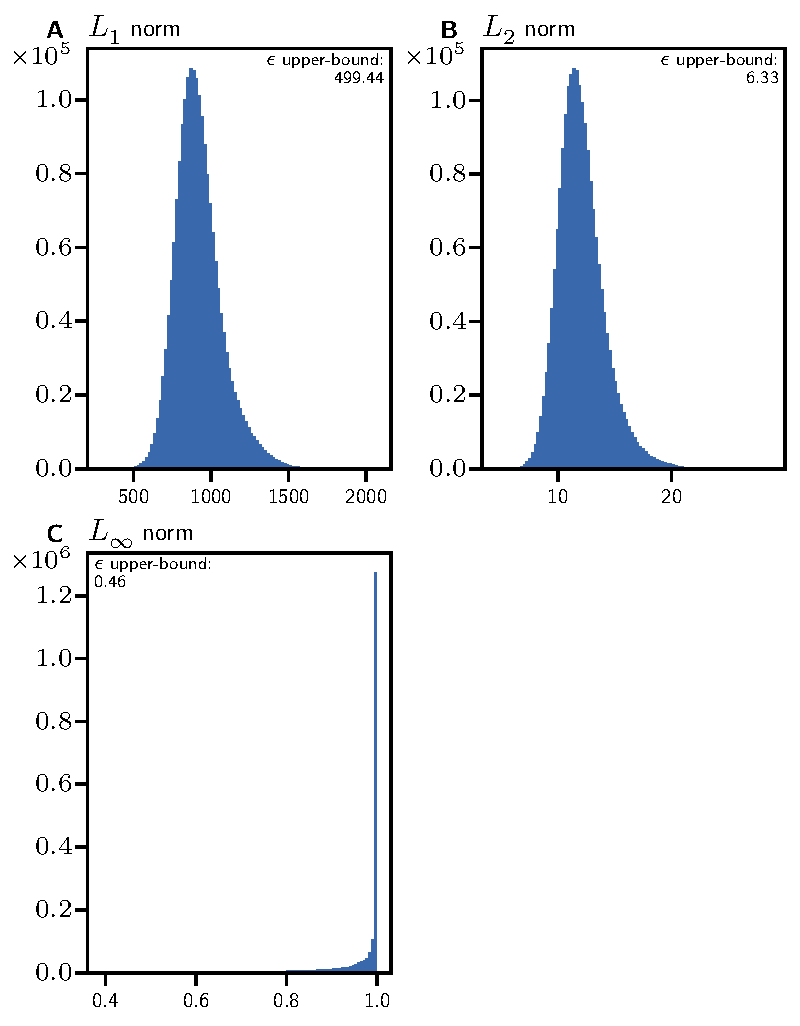
\includegraphics{distance_distribution_classes.pdf}
        \phantomcaption\label{fig:dist_cls_distibutionL1}
        \phantomcaption\label{fig:dist_cls_distibutionL2}
        \phantomcaption\label{fig:dist_cls_distibutionLiinf}
    \end{subcaptiongroup}
    \caption{Distances distributions of points in two different classes}\label{fig:dist_cls_distibution}
\end{figure}

\begin{figure}[htbp]
    \centering
    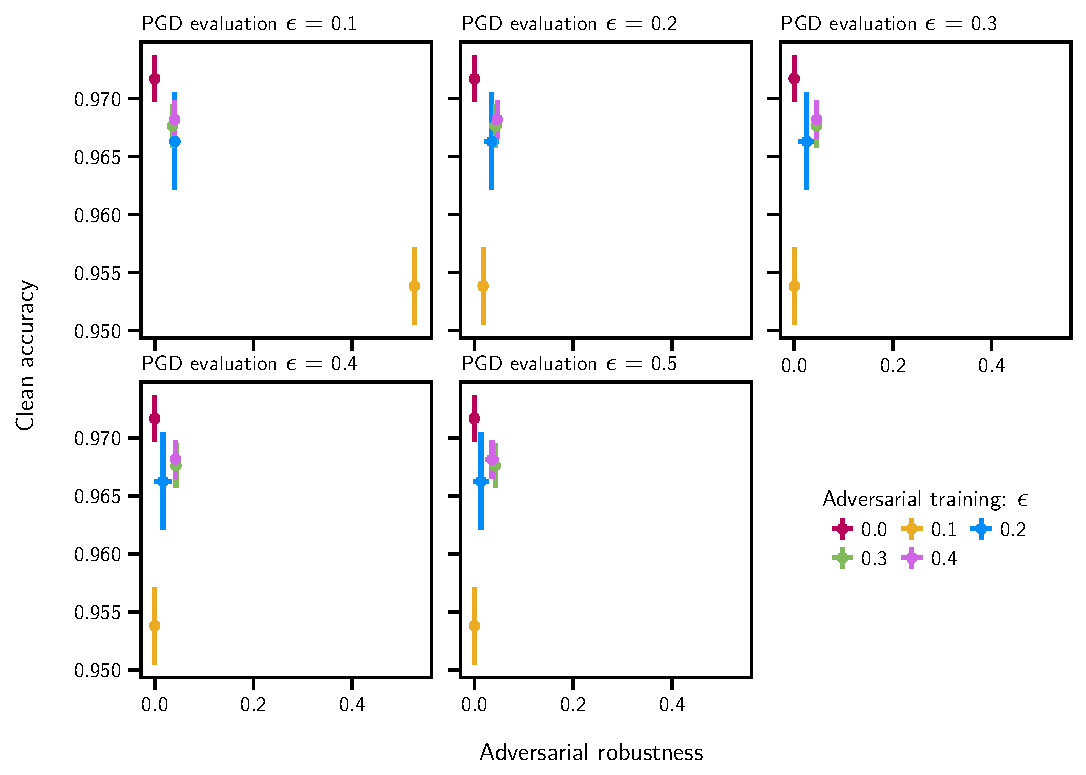
\includegraphics{MLP_LN_adversarial_tradeoff.pdf}
    \caption{<caption>}\label{fig:mlp_ln_adv_tradeoff}
\end{figure}

\begin{figure}[htbp]
    \centering
    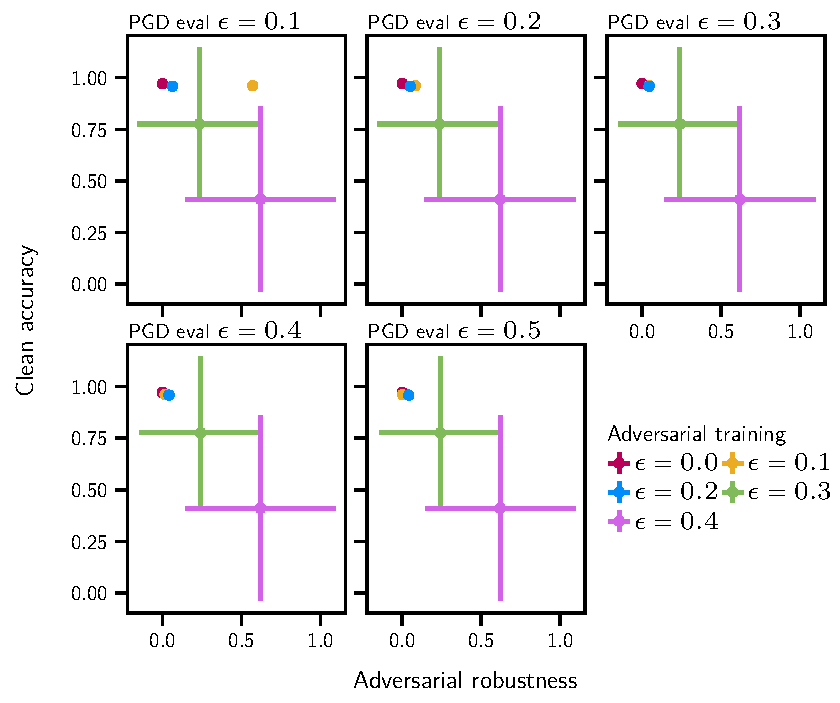
\includegraphics{MLP_NoNorm_adversarial_tradeoff.pdf}
    \caption{<caption>}\label{fig:mlp_nonorm_adv_tradeoff}
\end{figure}

\begin{figure}[htbp]
    \centering
    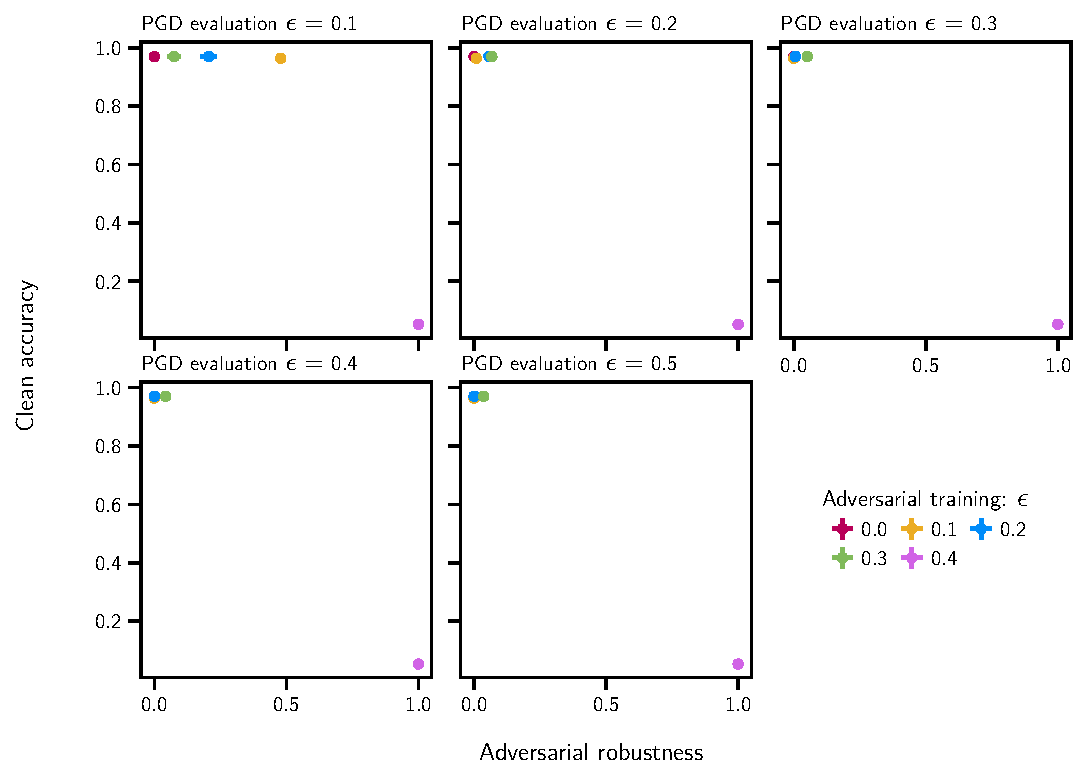
\includegraphics{MLP_FN_adversarial_tradeoff.pdf}
    \caption{<caption>}\label{fig:mlp_fn_adv_tradeoff}
\end{figure}

\begin{figure}[htbp]
    \centering
    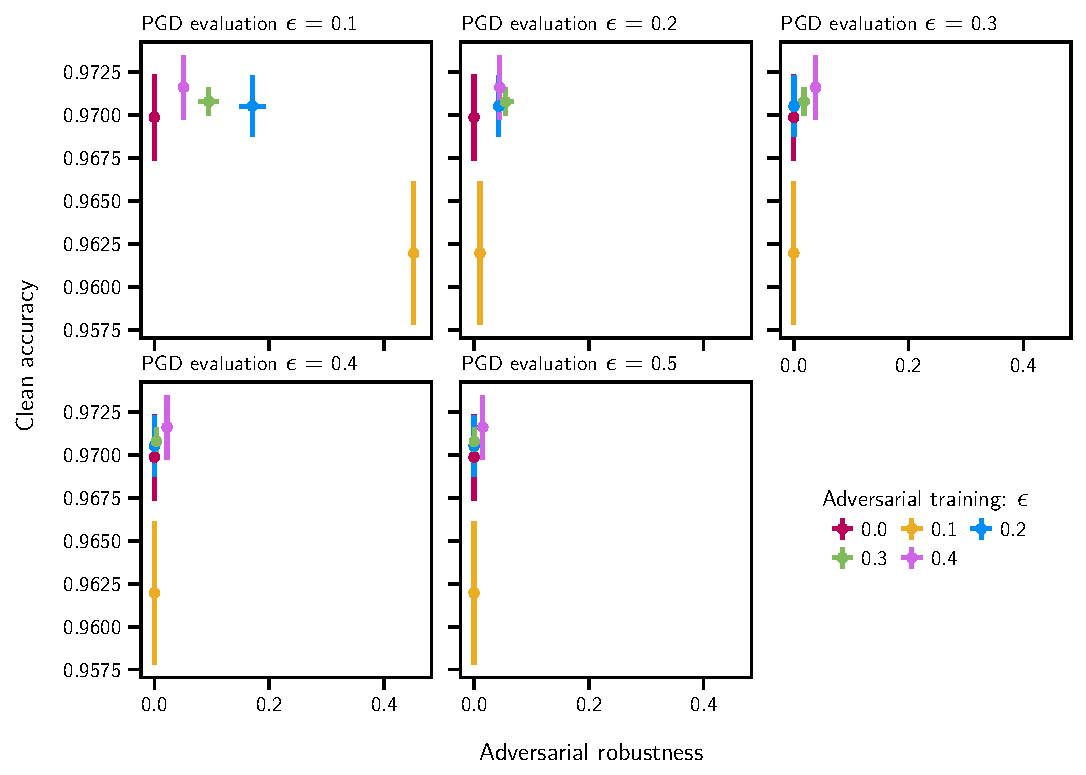
\includegraphics{MLP_FN_AGC_adversarial_tradeoff.pdf}
    \caption{<caption>}\label{fig:mlp_fnagcadv_tradeoff}
\end{figure}

\begin{landscape}
    \begin{figure}[htbp]
        \centering
        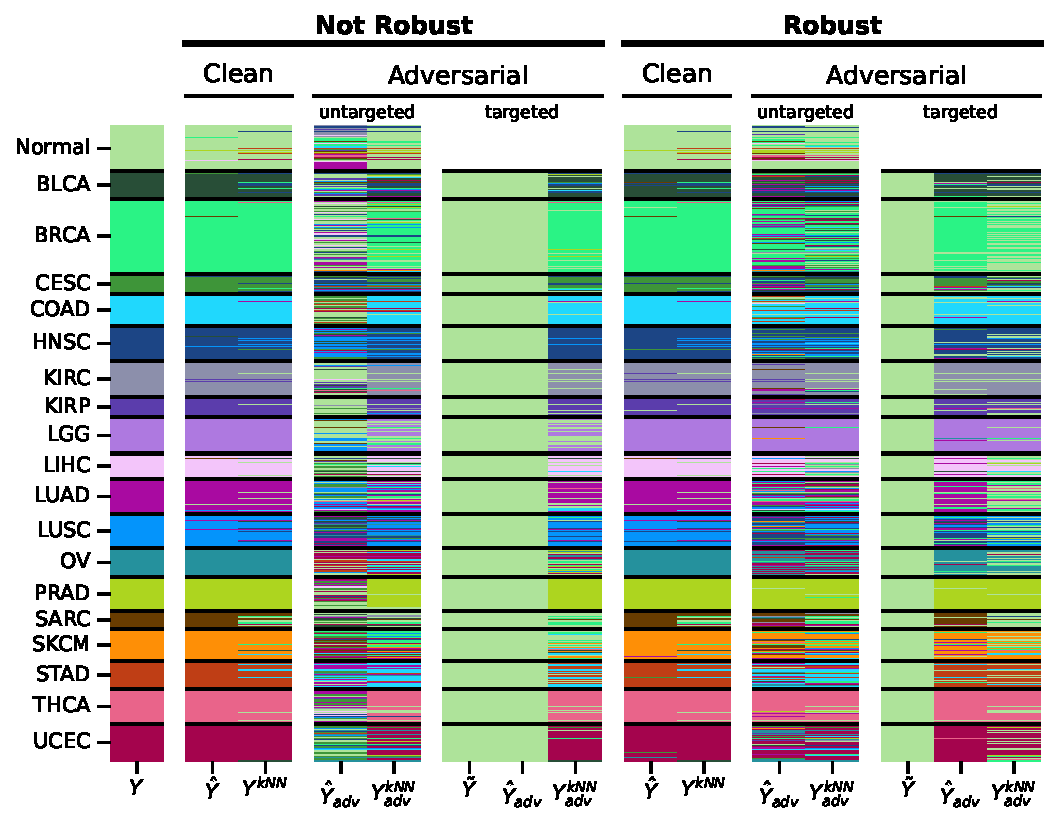
\includegraphics{MLP_LN_knn_comparison.pdf}
        \caption{<caption>}\label{fig:mlp_ln_knn_comp}
    \end{figure}

    \begin{figure}[htbp]
        \centering
        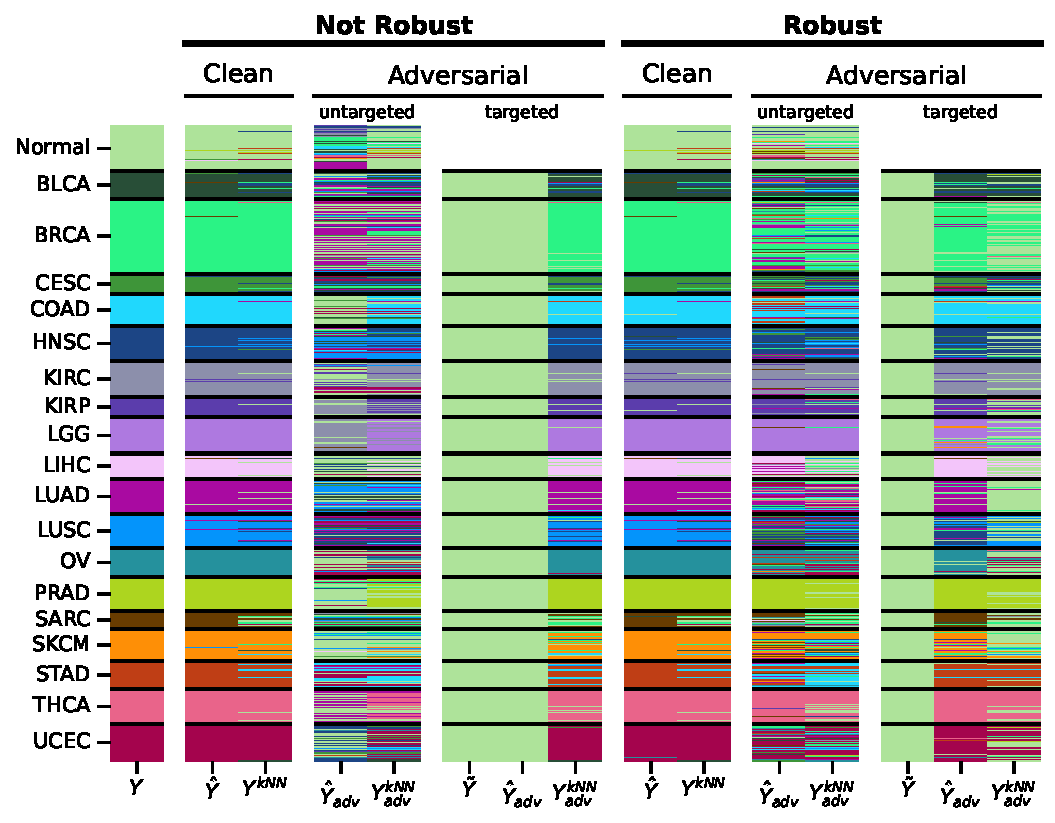
\includegraphics{MLP_NoNorm_knn_comparison.pdf}
        \caption{<caption>}\label{fig:mlp_nonorm_knn_comp}
    \end{figure}

    \begin{figure}[htbp]
        \centering
        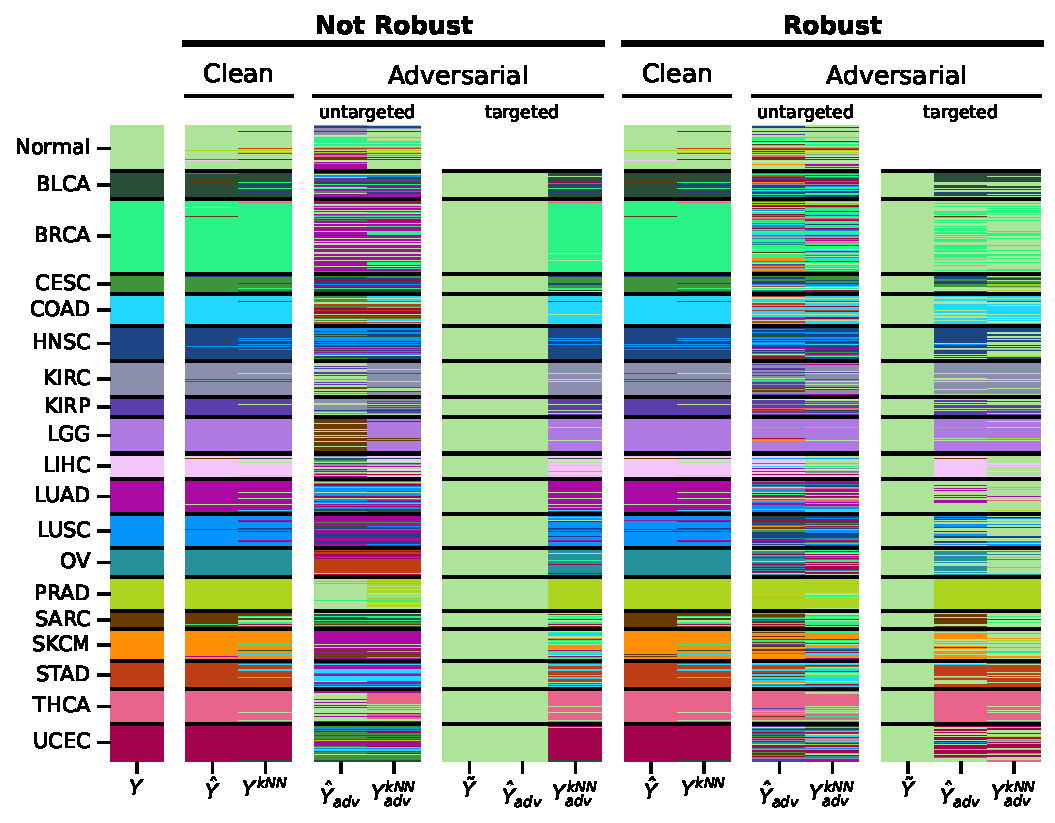
\includegraphics{MLP_FN_knn_comparison.pdf}
        \caption{<caption>}\label{fig:mlp_fn_knn_comp}
    \end{figure}

    \begin{figure}[htbp]
        \centering
        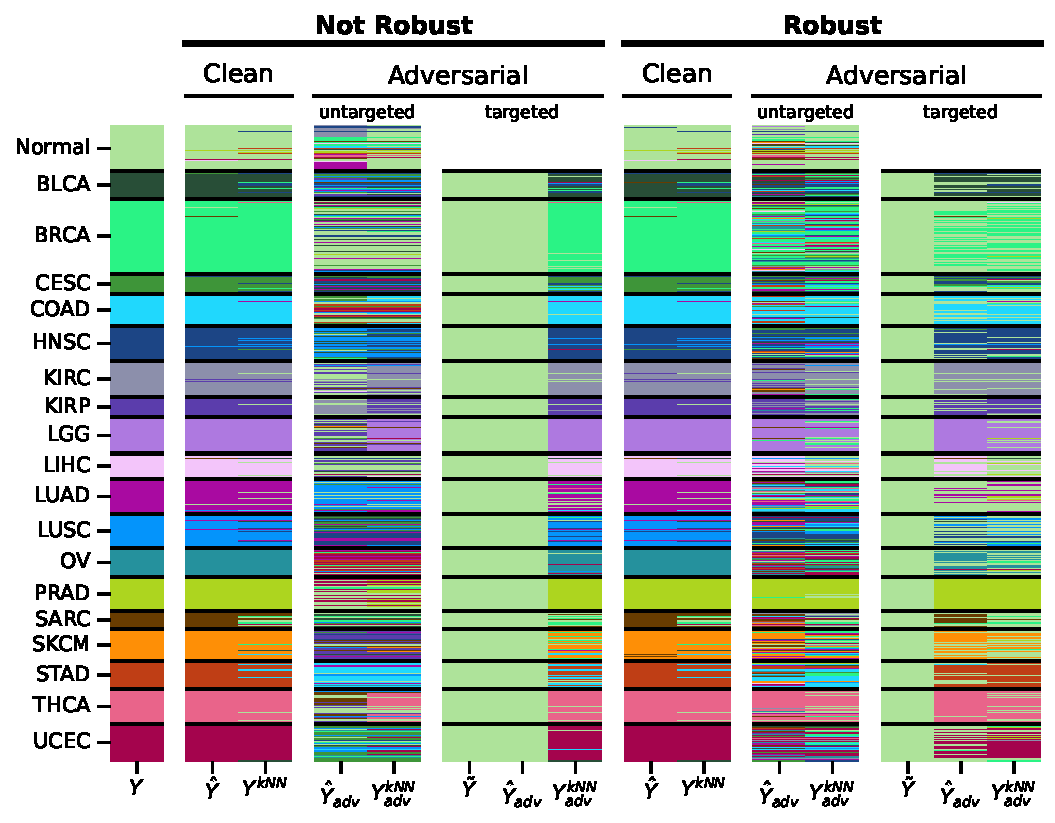
\includegraphics{MLP_FN_AGC_knn_comparison.pdf}
        \caption{<caption>}\label{fig:mlp_fnagc_knn_comp}
    \end{figure}
\end{landscape}
\backmatter
\end{document}
